%% 
%% Copyright 2019-2024 Elsevier Ltd
%% 
%% Version 2.4
%% 
%% This file is part of the 'CAS Bundle'.
%% --------------------------------------
%% 
%% It may be distributed under the conditions of the LaTeX Project Public
%% License, either version 1.2 of this license or (at your option) any
%% later version.  The latest version of this license is in
%%    http://www.latex-project.org/lppl.txt
%% and version 1.2 or later is part of all distributions of LaTeX
%% version 1999/12/01 or later.
%% 
%% The list of all files belonging to the 'CAS Bundle' is
%% given in the file `manifest.txt'.
%% 
%% Template article for cas-dc documentclass for 
%% double column output.

%\documentclass[a4paper,fleqn,longmktitle]{cas-dc}
\documentclass[a4paper,fleqn]{cas-dc}

%\usepackage[authoryear,longnamesfirst]{natbib}
%\usepackage[authoryear]{natbib}
%% Acta Astronautica reference style: numbers in square brackets, in the
%% order in which they appear in the text (see journal Guide for Authors).
\usepackage[numbers,sort&compress]{natbib}
\usepackage{float}
\usepackage{placeins}
\usepackage{caption}

%% cas-common.sty emits an "ORCID(s):" footnote unconditionally, which prints
%% as a dangling empty label when no \orcid fields are supplied. Suppress it
%% unless ORCIDs are actually present.
\ExplSyntaxOn
\RenewDocumentCommand \printorcid { }
{
  \seq_if_empty:NF \g_stm_orcid_seq
    {
      \group_begin:
        \tex_let:D \thefootnote \relax \footnotetext
        {
          \raggedright
          \textsc{orcid}(s):\c_space_token
          \seq_use:Nn \g_stm_orcid_seq { ;~ }
        }
      \group_end:
    }
}
\ExplSyntaxOff

%%%Author definitions
\def\tsc#1{\csdef{#1}{\textsc{\lowercase{#1}}\xspace}}
\tsc{WGM}
\tsc{QE}
\tsc{EP}
\tsc{PMS}
\tsc{BEC}
\tsc{DE}
%%%

\begin{document}
\pagestyle{plain}
\let\WriteBookmarks\relax
\def\floatpagepagefraction{1}
\def\textpagefraction{.001}
\shorttitle{Eclipse-Modulated Transient Energy Pumping in Near-Polar LEO for Spin-Stabilised Solar Sails}

\shortauthors{S. Vaahan et~al.}

\title [mode = title]{Eclipse-Modulated Transient Energy Pumping in Near-Polar Low Earth Orbit for Spin-Stabilised Solar Sails}                     
\tnotemark[1]

\tnotetext[1]{This document is the result of the work of the Orbital Mechanics Research Team within Project Svarog at Imperial College London.}


%% Shiki Vaahan, Ian Poon and Fatima Sajid are co-equal first authors
%% (\fnmark[1] -> \fntext[fn1]). Ian Poon is the corresponding author.
%% Affiliations are declared in order of first appearance in the author list,
%% so the printed superscripts a,b,c,... follow Elsevier convention.
\author[2]{Ian Poon}

\cortext[cor1]{Corresponding author: \href{mailto:ip323@ic.ac.uk}{ip323@ic.ac.uk}}
\fntext[fn1]{These authors contributed equally to this work.}

\affiliation[2]{organization={Department of Bioengineering, Imperial College London},
                city={London},
                country={UK}}



\begin{abstract}
This paper pursues two goals: to verify the existence of a passive orbital-energy-gain region for spin-stabilised solar sails in near-polar low Earth orbit (LEO), and to validate the open-source propagator used to map it against two independent flight-dynamics references: the industry-standard Ansys STK/Astrogator environment and the open-source Orekit library. Establishing such a regime with an inspectable, verified, and freely available toolchain matters because LEO has become the cost-effective testbed of choice for maturing solar- and drag-sail technology on low-cost CubeSat platforms, where reliable pre-flight prediction of the coupled solar-radiation-pressure (SRP) and drag dynamics is essential. Using a reduced analytical model and three-dimensional numerical propagations, we show that a bounded net-gain regime does exist, but only within a narrow region of LTDN--pitch space. At \(700\,\mathrm{km}\), only \(89\) of \(900\) sampled cases (\(\sim 10\%\)) exhibit positive semi-major-axis excursion within the \(14\)-day analysis window, with the strongest case reaching \(\Delta a \approx +20.07\,\mathrm{km}\) at LTDN \(12.266\,\mathrm{h}\) and pitch \(24.8^\circ\). Eclipse is causally decisive: for the representative gain case the eclipse-on trajectory reaches \(\Delta a \approx +10.31\,\mathrm{km}\) by day \(14\), whereas the eclipse-off counterpart falls to \(\Delta a \approx -47.75\,\mathrm{km}\); orbit-resolved SRP work diagnostics show that gain occurs only when eclipse suppresses predominantly negative-work portions of the SRP cycle. Longer-horizon propagation shows the effect is transient and self-limiting: the representative gain case peaks at \(7098.211\,\mathrm{km}\) on day \(26.50\) before declining to \(7064.717\,\mathrm{km}\) by day \(75\), below its initial \(7078.137\,\mathrm{km}\), as apogee pumping, perigee erosion, and eccentricity growth progressively increase drag exposure and weaken the favourable SRP projection. Independent open-source and Orekit propagators both reproduce the gain lobe, the eclipse-driven sign reversal, and the transient--breakdown signature, confirming that the mechanism is not a numerical artefact. Cross-validation against STK shows that two-body and \(J_2\) dynamics agree to better than \(0.05\,\mathrm{km}\) over 14 days, while the drag-induced decay differs by close to an order of magnitude despite matching instantaneous force; the second reference resolves that ambiguity, since Orekit reproduces the open-source \(14\)-day decay to \(4\times10^{-10}\,\mathrm{km}\), localising the discrepancy to STK's drag application rather than to the open-source implementation. Orekit also passes the test STK could not: its N-plate SRP model does couple to an inertially-fixed sail attitude, so the passive-sail SRP dynamics are confirmed against a second tool rather than only analytically. Isolating each modelling choice in turn shows that atmosphere co-rotation and the geodetic-versus-geocentric altitude convention shift the \(14\)-day decay by at most \(19\%\), whereas substituting a different atmosphere model changes it by factors up to \(5.9\) --- identifying the choice of atmospheric density model, rather than the SRP mechanism or the drag conventions, as the dominant uncertainty governing where the regime is realisable. A further numerical caveat emerges: because a binary umbra makes the SRP force discontinuous, fixed-step integration converges at first rather than fourth order and overstates the gain, appreciably so at the step sizes large sweeps encourage. The paper therefore establishes a validated but narrow result: eclipse timing can enable a real, bounded, transient energy-pumping regime in near-polar LEO, its existence is robust across independent propagators, and its quantitative threshold is drag-model dependent. The full toolchain and data are released openly.
\end{abstract}

\begin{highlights}
\item Passive solar sails can gain semi-major axis transiently in near-polar LEO.
\item Gain exists only in a narrow LTDN--pitch band; eclipse timing enables it.
\item Apogee pumping, eccentricity growth and perigee erosion make it self-limiting.
\item Open-source propagator reproduces the gain lobe and eclipse causality.
\item STK cross-check validates $J_2$ below 0.05 km over 14 d; drag dominates error.
\end{highlights}


%% Acta Astronautica allows a maximum of 6 keywords.
\begin{keywords}
Solar sail \sep Low Earth orbit \sep Solar radiation pressure \sep Eclipse \sep Open-source propagator \sep Model validation
\end{keywords}



\maketitle

\section{Introduction}
\FloatBarrier
\noindent Solar radiation pressure (SRP) provides a continuous, propellant-free means of modifying spacecraft orbits, and has been demonstrated in missions including IKAROS \citep{tsuda2011ikaros,sawadaMissionReportSolar2011}, LightSail~2 \citep{spencerLightSail2Solar2021}, and the Advanced Composite Solar Sail System \citep{wilkieOverviewNASAAdvanced2021}. Recent reviews summarise the current state of solar sailing technology and mission heritage \citep{johnsonSolarSailsTechnology2012,yakezerashviliRecentAdvancesSpace2025}. While active solar sailing enables controlled trajectory shaping, the possibility of achieving meaningful orbital energy change under purely passive configurations remains less well understood, particularly in low Earth orbit (LEO) where atmospheric drag and gravitational perturbations are significant. The use of solar sails in LEO has been explored for deorbiting \citep{stohlmanDevelopmentDeorbitsailFlight2014,lucking2012solar} and for altitude maintenance \citep{berthetSunflowerMissionConcept2023}, but the short-horizon interaction between eclipse timing and SRP work balance has received limited attention.

\vspace{0.5em}
\par\noindent Prior work has examined the coupled effects of solar radiation pressure and atmospheric drag on high area-to-mass spacecraft. In particular, \citet{colombomcinnes} demonstrated that asymmetric SRP, including the influence of Earth eclipse, can be exploited to balance drag losses and produce long-lived Earth-centred orbits without active control. The influence of SRP on high area-to-mass ratio objects has also been studied in the context of long-term orbit evolution and resonance structures \citep{valk2008semi}. These analyses highlight the importance of SRP–drag interaction and shadow-induced asymmetries in shaping orbital evolution. However, much of the existing SRP–drag literature emphasizes long‑term or averaged behavior and equilibrium‑like manifolds or ``balance'' conditions, rather than isolating short‑horizon regimes in which the timing of eclipse arcs alters the sign and magnitude of orbit‑averaged SRP work.

\vspace{0.5em}
\par\noindent In near-polar LEO, the interaction between SRP, atmospheric drag, Earth’s oblateness ($J_2$), and eclipse timing produces a dynamically coupled environment in which small perturbations can lead to non-intuitive orbital behaviour over short timescales \citep{prieto2014drag}. In particular, a passively oriented, spin-stabilised sail experiences alternating phases of positive and negative SRP work over each orbit, which would be expected to largely cancel in the absence of asymmetries \citep{mcinnes1999}.

\vspace{0.5em}
\par\noindent However, eclipse introduces a temporal modulation of SRP by removing solar forcing over specific orbital arcs \citep{hubaux2013shadow}. Depending on the orbital geometry, this can selectively suppress phases in which SRP performs negative work, altering the orbit-averaged energy balance. This raises the question of whether a net increase in semi-major axis can arise over a bounded time horizon under restricted conditions, without active attitude control.

\vspace{0.5em}
\par\noindent This work investigates that question by isolating and characterising a transient, geometry-dependent energy-pumping regime in near-polar LEO for spin-stabilised solar sails. The aim is not to propose a mission architecture or demonstrate sustained orbit raising, but to identify where the regime exists, explain the eclipse-modulated SRP work-imbalance mechanism, and quantify the conditions under which it appears and breaks down. Using a reduced-order dynamical model and parameter-space sweeps over local time of descending node (LTDN) and sail orientation, we show that short-horizon semi-major-axis growth can occur within a narrow alignment envelope, but that the effect is inherently self-limiting through coupled eccentricity growth, increased drag exposure near perigee, and gradual drift in Sun-relative geometry.
\FloatBarrier

\begin{figure*}[t]
    \centering
 
    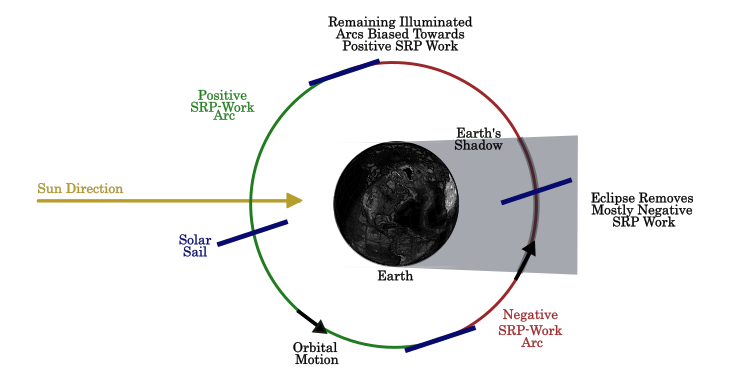
\includegraphics[width=1\linewidth]{Figures/earth.png}
    \vspace{-1.5em}
    \caption{Conceptual schematic of the eclipse-modulated SRP work asymmetry in the reduced mechanism picture. For an inertially fixed sail, solar radiation pressure contributes positive work over part of the illuminated orbit and negative work over another part. If eclipse removes a larger fraction of the unfavourable arc than of the favourable arc, the one-orbit SRP work integral becomes positive. The figure is intended to illustrate the phase-selective gating mechanism, not to represent the full propagated 3D geometry directly.}
    \label{fig:placeholder}
\end{figure*}

\vspace{-1em}
\section{Scope and Problem Definition}
\vspace{-0.5em}

\noindent This work is framed as a bounded orbital-dynamics study of a specific short-horizon regime in near-polar LEO in which solar radiation pressure (SRP) can, under restricted passive conditions, produce a net orbit-averaged energy gain. The system considered is intentionally limited to the coupled effects of central gravity, Earth’s oblateness (\(J_2\)), atmospheric drag, solar radiation pressure, and eclipse-modulated shadowing, for a spin-stabilised sail whose orientation is fixed in inertial space and not actively controlled.

\vspace{0.5em}
\par\noindent The primary question is whether eclipse timing can, over a bounded horizon, produce a net positive orbit-averaged energy input by selectively suppressing phases of negative SRP work, and how strongly that effect depends on orbital geometry. The purpose is therefore to isolate and explain a geometric dynamical mechanism, not to demonstrate an operational orbit-raising strategy.

\vspace{0.5em}
\par\noindent The study is framed around two explicit objectives. The first (scientific) objective is to \emph{verify the existence} of the passive-gain region: to map the constrained dynamical regime, explain its underlying eclipse-modulated SRP work-imbalance mechanism, and determine the conditions under which the observed energy gain emerges and subsequently breaks down. The second (methodological) objective is to \emph{validate the open-source propagator} used for the first: to cross-check its force models, component by component, against the industrial flight-dynamics tool STK Astrogator and against the independent open-source library Orekit, and to quantify where the tools agree and diverge. The two objectives are complementary --- the validation establishes that the gain region is reproducible across independent tools and identifies which force-model choices most strongly govern the result.

\vspace{0.5em}
\par\noindent Several exclusions are imposed to maintain a controlled scope. This study does not claim disposal-compliant mission design, communications-feasible spacecraft architecture, collision-risk-assessed operations, maintenance of an exact Sun-synchronous orbit, or long-term sustained orbit raising. It does not attempt subsystem-level mission design, active attitude-control implementation, or guidance and feedback control. The external validation performed here is a component-level cross-check of the propagator's force models against STK Astrogator and Orekit, not a flight-data validation of the mission concept; the results should therefore not be interpreted as a demonstrated mission concept, but as evidence for a bounded dynamical effect within the modelled regime, together with a verified toolchain for studying it. Sun-synchronous-like initial conditions are used only to impose a controlled and interpretable Sun-relative geometry; they are not intended to assert that the vehicle remains on an exactly maintained operational SSO throughout the propagation.
\FloatBarrier



\section{Physical Mechanism of Eclipse-Modulated \newline Energy Pumping}
\label{sec:physics}
\FloatBarrier
\noindent This section introduces a reduced analytical picture to isolate the core geometric mechanism by which eclipse timing can bias solar-radiation-pressure (SRP) work over an orbit. Its purpose is not to derive a design-optimal sail orientation for the full propagated problem, nor to replace the later 3D simulations, but to establish the sign logic of phase-selective forcing in the simplest setting where it can be seen clearly. The full numerical problem considered later includes three-dimensional orbital geometry, \(J_2\)-driven nodal precession, drag, eclipse-modulated illumination, and coupled evolution of the orbital elements; the reduced model is therefore used here only as a mechanistic scaffold for interpreting those results.

\vspace{-0.5em}
\par\noindent The reduced argument developed below is used to identify the sign structure of the SRP work integral under eclipse-modulated illumination, and thereby to motivate the later propagated results.

\vspace{0.5em}
\subsection{\textbf{Orbital energy change and transverse work}}

\noindent The central quantity of interest is the sign of the orbit-averaged transverse SRP work, because the Gauss variational equation for semi-major axis \citep{vallado2007,battin1999} directly links \(da/dt\) to the radial and transverse components of the perturbing acceleration. Writing the perturbing acceleration in the local orbital frame as radial (\(F_R\)), transverse (\(F_T\)), and normal (\(F_N\)) components, the semi-major-axis equation is
\begin{equation}
\frac{da}{dt} = \frac{2a^2}{h}\left[e\sin\theta\,F_R + (1+e\cos\theta)\,F_T\right],
\label{eq:da_gve}
\end{equation}
where $F_R$ and $F_T$ are the radial and transverse components of the perturbing acceleration, $\theta$ is the true anomaly, $a$ is the semi-major axis, and $h$ is the specific angular momentum.

\vspace{0.5em}
\par\noindent For near-circular low Earth orbits ($e\approx 0$), this reduces to
\begin{equation}
\frac{da}{dt} \approx \frac{2a^2}{h}F_T = \frac{2}{n}F_T,
\label{eq:da_circular}
\end{equation}
where $n=\sqrt{\mu/a^3}$ is the mean motion. The semi-major axis evolution is therefore governed primarily by the transverse component of the perturbing force. Equivalently, since the specific orbital energy is
\begin{equation}
\varepsilon = -\frac{\mu}{2a},
\end{equation}
its rate of change is
\begin{equation}
\dot{\varepsilon} = \mathbf{a}_{p}\cdot\mathbf{v} = F_T v,
\label{eq:energy_rate}
\end{equation}
for a circular orbit, where $\mathbf{a}_{p}$ is the perturbing acceleration and $v=\sqrt{\mu/a}$ is the orbital speed. Hence, in the near-circular setting used here, positive transverse work corresponds to increasing orbital energy and increasing semi-major axis, while negative transverse work has the opposite effect.

\vspace{0.5em}
\par\noindent This makes the sign of the orbit-averaged transverse work the central quantity of interest in the reduced mechanism. In particular, if the SRP contribution satisfies
\begin{equation}
\int_0^T F_T\,dt > 0,
\end{equation}
over one orbital period \(T\), then the orbit-integrated SRP work is positive and the corresponding one-orbit change in orbital energy, and hence in semi-major axis, is favourable.

\vspace{0.5em}
\subsection{\textbf{Passive symmetry and cancellation in the fully illuminated case}}

\noindent Consider first an idealised 2D planar circular orbit with the Sun fixed in inertial space. Let the Sun direction define the $+x$ axis, and parameterise the spacecraft position and velocity by
\begin{equation}
\mathbf{r}=r(\cos\theta,\sin\theta), \qquad
\mathbf{v}=v(-\sin\theta,\cos\theta),
\end{equation}
where $\theta$ is the orbital phase measured from the sunward direction. For a passively oriented, spin-stabilised sail with fixed inertial attitude, let the sail normal be
\begin{equation}
\mathbf{n}=(\cos\beta,\sin\beta),
\end{equation}
where $\beta$ is the constant pitch angle measured from the Sun line.

\vspace{0.5em}
\par\noindent For an ideal reflecting sail under constant illumination, the SRP acceleration has fixed inertial direction and may be written in the form \citep{mcinnes1999}
\begin{equation}
\mathbf{a}_{\text{SRP}} = a_0 \cos^2\beta \,\mathbf{n},
\label{eq:srp_vector}
\end{equation}
where $a_0$ is the characteristic SRP acceleration scale. The instantaneous specific power is then
\begin{equation}
\dot{\varepsilon} = \mathbf{a}_{\text{SRP}}\cdot\mathbf{v}
= a_0\cos^2\beta\,\mathbf{n}\cdot\mathbf{v}.
\end{equation}
Substituting for $\mathbf{n}$ and $\mathbf{v}$ gives
\begin{equation}
\mathbf{n}\cdot\mathbf{v}
= v(-\sin\theta\cos\beta + \cos\theta\sin\beta)
= v\sin(\beta-\theta),
\end{equation}
so that
\begin{equation}
\dot{\varepsilon} = a_0 v \cos^2\beta \,\sin(\beta-\theta).
\label{eq:power_phase}
\end{equation}

\vspace{0.5em}
\par\noindent Over a fully illuminated circular orbit, using $dt=(r/v)\,d\theta$, the net specific energy change is
\begin{equation}
\Delta\varepsilon_{\text{full}}
= \int_0^{2\pi}\dot{\varepsilon}\,dt
= a_0 r \cos^2\beta \int_0^{2\pi}\sin(\beta-\theta)\,d\theta.
\end{equation}
Since
\begin{equation}
\int_0^{2\pi}\sin(\beta-\theta)\,d\theta = 0,
\end{equation}
it follows that
\begin{equation}
\Delta\varepsilon_{\text{full}} = 0.
\label{eq:full_cancellation}
\end{equation}

\vspace{0.5em}
\par\noindent Equation~\eqref{eq:full_cancellation} formalises the passive symmetry argument: under continuous illumination, a fixed-attitude sail experiences alternating orbital phases of positive and negative transverse work that cancel exactly over one revolution. In this idealised baseline case, the one-orbit net change in orbital energy vanishes despite non-zero instantaneous SRP forcing.

\vspace{0.5em}
\subsection{\textbf{Eclipse as a selective gating mechanism}}

\noindent The previous cancellation result changes fundamentally once eclipse is introduced. In a midnight orbit under a cylindrical shadow model, the eclipse is centred on the anti-solar direction $\theta=\pi$ and spans the interval
\begin{equation}
\theta \in [\pi-\delta,\pi+\delta],
\qquad
\delta = \arcsin\left(\frac{R_E}{r}\right),
\label{eq:eclipse_bounds}
\end{equation}
where $R_E$ is the Earth radius and $r$ is the orbital radius. The illuminated arcs are therefore
\begin{equation}
[0,\pi-\delta]\cup[\pi+\delta,2\pi].
\end{equation}

\vspace{0.5em}
\par\noindent The net specific energy change over the illuminated portion of the orbit becomes
\begin{equation}
\Delta\varepsilon_{\text{lit}}
= a_0 r \cos^2\beta
\left[
\int_0^{\pi-\delta}\sin(\beta-\theta)\,d\theta
+
\int_{\pi+\delta}^{2\pi}\sin(\beta-\theta)\,d\theta
\right].
\label{eq:lit_integral}
\end{equation}
Using the full-orbit cancellation result, this may be written more compactly as minus the contribution from the shadowed arc,
\begin{equation}
\Delta\varepsilon_{\text{lit}}
=
- a_0 r \cos^2\beta
\int_{\pi-\delta}^{\pi+\delta}\sin(\beta-\theta)\,d\theta.
\end{equation}
Evaluating the integral gives
\begin{equation}
\int_{\pi-\delta}^{\pi+\delta}\sin(\beta-\theta)\,d\theta
= 2\sin\beta\,\sin\delta,
\end{equation}
and hence
\begin{equation}
\Delta\varepsilon_{\text{lit}}
=
-2a_0 r \cos^2\beta\,\sin\beta\,\sin\delta.
\label{eq:delta_e_final}
\end{equation}

\vspace{0.5em}
\par\noindent Equation~\eqref{eq:delta_e_final} shows explicitly that eclipse does not merely reduce the SRP magnitude; it breaks the passive cancellation by removing a finite interval of orbital phase from the work integral. The sign of the net energy change is therefore controlled by the sign of \(-\sin\beta\). In this 2D midnight-orbit idealisation,
\begin{equation}
\Delta\varepsilon_{\text{lit}} > 0
\qquad\Longleftrightarrow\qquad
\sin\beta < 0.
\end{equation}
A finite branch of pitch angles therefore exists for which eclipse suppresses unfavourable work more strongly than favourable work, leaving a positive residual contribution to the one-orbit SRP work balance and hence a positive one-orbit energy change.

\vspace{0.5em}
\par\noindent Within this reduced 2D midnight-orbit model, the magnitude of the one-orbit energy gain is maximised by maximising \(-\sin\beta\cos^2\beta\), which gives
\begin{equation}
\sin^2\beta = \frac{1}{3},
\end{equation}
with the positive-gain branch
\begin{equation}
\beta^\star = -\arcsin\left(\frac{1}{\sqrt{3}}\right)\approx -35.3^\circ.
\end{equation}
This result is used here only to show that the eclipse-modulated work imbalance is not marginal or accidental in the reduced geometry. It is not claimed to be a design optimum for the full propagated 3D system, whose geometry, illumination history, drag losses, and coupled element evolution are substantially richer.



\vspace{0.5em}
\subsection{\textbf{Dependence on orbital geometry}}

\noindent The reduced mechanism is intrinsically phase-selective and therefore strongly dependent on orbital geometry. In the full problem, the local time of descending node (LTDN), the Sun-relative orientation of the orbital plane, and the fixed sail attitude together determine which parts of the orbit are illuminated, which are shadowed, and how the SRP work distribution is sampled. The sign and magnitude of the orbit-integrated SRP contribution therefore depend on whether eclipse preferentially removes unfavourable or favourable work phases.

\vspace{0.5em}
\par\noindent The midnight case is analytically useful because the eclipse is centred on the anti-solar point and the resulting shadow interval is symmetric in orbital phase, allowing the effect of selective gating to be shown in closed form. Away from this limiting geometry, the illuminated and shadowed arcs shift relative to the SRP work distribution, and the balance between positive and negative transverse work changes accordingly. Net semi-major-axis growth is therefore expected only over restricted regions of the full parameter space.

\vspace{0.5em}
\par\noindent Crucially, the same phase-dependent forcing that produces a favourable one-orbit SRP work imbalance need not produce shape-preserving orbit raising. Gauss' variational equations imply that the detailed phasing of \(F_R\) and \(F_T\) can simultaneously drive changes in eccentricity and related orbital geometry, while out-of-plane forcing in the full 3D problem affects inclination and node. A positive orbit-averaged SRP work contribution is therefore not equivalent to uniform upward translation of the orbit. In the propagated cases examined later, the same eclipse-biased phasing that produces transient semi-major-axis gain can coexist with eccentricity growth, altered perigee and apogee behaviour, and ultimately degradation of the gain regime.
\vspace{0.5em}


\subsection{Transient nature of the mechanism}
\noindent The reduced analysis establishes only that eclipse can bias the one-orbit SRP work balance in favour of net energy gain for restricted geometries. It does not establish persistence, monotonic orbit raising, or long-horizon robustness once the full coupled dynamics are restored. The propagated 3D results therefore test whether this favourable work asymmetry survives in realistic near-polar LEO motion, and how it breaks down through coupled changes in eccentricity, drag exposure, and Sun-relative geometry; these longer-horizon effects are examined in Section~\ref{sec:breakdown}.
\FloatBarrier

\section{Dynamical model and assumptions}
\label{sec:model}
\FloatBarrier
\noindent This study considers a bounded orbital-dynamics problem in near-polar low Earth orbit (LEO) intended to isolate the short-horizon interaction between solar radiation pressure (SRP), eclipse timing, atmospheric drag, and \(J_2\)-driven nodal precession. The emphasis is on whether a sail with inertially fixed orientation can exhibit short-horizon semi-major-axis growth while remaining close to Sun-synchronous orbital geometry.

\vspace{5pt}
\par\noindent A Sun-synchronous orbit (SSO) is desirable because it maintains a predictable Sun-relative geometry while allowing the orbital plane to precess with the apparent annual motion of the Sun \citep{vallado2007}. For near-circular LEO, this requires a secular right ascension of the ascending node (RAAN) precession rate of approximately
\begin{equation}
\frac{d\Omega}{dt} \approx 0.986^\circ/\text{day},
\label{eq:RAANrate}
\end{equation}
which is primarily supplied by Earth’s oblateness through the \(J_2\) perturbation. The corresponding nodal precession rate is \citep{vallado2007}
\begin{equation}
\dot{\Omega}
  = -\frac{3}{2}\,J_2\,
      \left(\frac{R_{E}}{a\bigl(1-e^{2}\bigr)}\right)^{\!2}
      \sqrt{\frac{\mu}{a^{3}}}\,
      \cos i.
\end{equation}
For circular orbits (\(e=0\)) in the altitude range considered here, the inclination required to satisfy Eq.~\eqref{eq:RAANrate} is close to \(98^\circ\), as summarised in Table~\ref{tab:sso_inclinations}.


\begin{table*}[htbp]
\centering
\caption{Required inclination to maintain Sun-synchronous orbits (SSO) for circular orbits (\(e = 0\)) at selected altitudes.}\label{tab:sso_inclinations}
\vspace{1em}
\begin{tabular}{c|c}
\textbf{Altitude (km)} & \textbf{Required Inclination (°)} \\
\hline
600 & 97.92 \\
700 & 98.04 \\
800 & 98.17 \\
900 & 98.31 \\
\end{tabular}

\end{table*}


\begin{table*}[htbp]
\centering
\caption{Baseline parameters used for the representative gain-case propagation and local mechanism analysis.}
\label{tab:baseline_params}
\vspace{0.5em}
\begin{tabular}{l c}
\hline
\textbf{Parameter} & \textbf{Value} \\
\hline
Initial altitude, \(h_0\) & \(700\,\mathrm{km}\) \\
Initial inclination, \(i_0\) & \(98.17^\circ\) \\
Initial eccentricity, \(e_0\) & \(1\times10^{-4}\) \\
Spacecraft mass, \(m\) & \(10\,\mathrm{kg}\) \\
Sail area, \(A\) & \(100\,\mathrm{m^2}\) \\
Area-to-mass ratio, \(A/m\) & \(10\,\mathrm{m^2\,kg^{-1}}\) \\
Reflectivity coefficient, \(C_r\) & \(1.7\) \\
Drag coefficient, \(C_D\) & \(2.2\) \\
\hline
\end{tabular}
\end{table*}

\vspace{5pt}
\par\noindent In the present work, the sail orientation is prescribed as inertially fixed over the time horizons of interest, and no active steering law is applied during propagation. This contrasts with actively steered sails \citep{dachwaldOptimalSolarSail2005,quartaOptimalInterplanetaryTrajectories2023} and with active momentum management approaches such as those developed for Solar Cruiser \citep{cannellaDesignOverviewSolar2021,shenSolarSailMomentum2026}. The fixed-attitude assumption is deliberate: it allows the orbital consequences of a fixed force geometry to be isolated directly, without introducing control-law dependence into the interpretation of the results. At the same time, it imposes an important limitation. As the orbital plane precesses and the Sun-relative geometry evolves, the orientation of the sail with respect to both the Sun and the local orbital frame cannot remain optimal indefinitely. Any favourable energy-transfer regime must therefore be understood as geometry-bounded and transient rather than as a permanently sustained operating mode.



\vspace{5pt}
\par\noindent The evolution of the orbit under weak non-Keplerian perturbations is interpreted using the Gauss Variational Equations (GVEs) \citep{vallado2007,battin1999}. Writing the perturbing acceleration vector \( \vec{F} \) in the local orbital frame as radial (\(F_R\)), transverse (\(F_T\)), and normal (\(F_N\)) components, the orbital-element evolution is given by
\begin{equation}
\frac{da}{dt} = \frac{2a^2}{h} \left[ e \sin{\theta} \, F_R + (1 + e \cos{\theta}) \, F_T \right],
\label{eq:da}
\end{equation}
\begin{equation}
\frac{de}{dt} = \frac{\mu}{h} \left[ \sin{\theta} \, F_R + \left( \cos{\theta} + \frac{e + \cos{\theta}}{1 + e \cos{\theta}} \right) F_T \right]
\end{equation}
\begin{equation}
\frac{di}{dt} = \frac{r \cos{u}}{h} \, F_N,
\label{eq:di}
\end{equation}
\begin{equation}
\frac{d\Omega}{dt} = \frac{r \sin{u}}{h \sin{i}} \, F_N,
\label{eq:domega}
\end{equation}
where \( h = \sqrt{\mu a (1 - e^2)} \) is the specific angular momentum, \( r = a(1 - e^2)/(1 + e \cos{\theta}) \) is the instantaneous orbital radius, \( \theta \) is the true anomaly, and \( u = \omega + \theta \) is the argument of latitude. A detailed derivation of the GVEs is given by \citet{vallado2007}.

\vspace{5pt}
\par\noindent These expressions clarify the role of each perturbing component. In near-circular LEO, semi-major-axis growth is driven primarily by the in-plane force, especially the transverse component \(F_T\), whereas inclination \(i\) and RAAN \(\Omega\) evolve through the normal component \(F_N\). Since Sun-synchronicity relies on the secular \(J_2\)-driven nodal precession described above, additional out-of-plane forcing should remain small if the orbit is to stay close to the desired SSO geometry.

\vspace{5pt}
\par\noindent This creates the central geometrical tension of the present study. To obtain semi-major-axis growth, the sail must produce a favourable in-plane force with a strong transverse projection, while remaining close to SSO requires the normal component \(F_N\) to stay limited. Because the sail orientation is fixed in inertial space, the Sun-relative cone angle and the orbital-frame force decomposition drift as the orbit evolves, so any favourable geometry is expected to persist only over a bounded interval.

\vspace{5pt}
\par\noindent % [PLACEHOLDER: Figure showing the time evolution of the SRP force decomposition in the orbital frame for a representative gain case. This should show \(F_T\) and \(F_N\) over time, or equivalently the Sun-relative geometric drift, to support the claim that favourable in-plane forcing is temporary.]
The force model retained for this study is intentionally simple and is chosen to isolate the mechanism of interest rather than to maximise environmental fidelity. The translational dynamics include central gravity, Earth’s oblateness through the \(J_2\) term, solar radiation pressure, eclipse shadowing, and atmospheric drag. No Earth albedo model is included.

\vspace{7pt}
\noindent\textbf{Solar radiation pressure} \vspace{2pt}

\par\noindent The SRP model is based on photon momentum transfer to a reflective flat plate \citep{mcinnes1999}. For an idealised square sail with cone angle \( \alpha \) relative to the Sun line, the force magnitude follows the familiar \( \cos^2\alpha \) dependence for a flat-plate sail (see \citealp{mcinnes1999}, Ch.~2). In the implementation used here, the SRP acceleration is written as
\begin{equation}
    \mathbf{a}_{\text{SRP}} = \frac{P_{1\ \text{AU}} \, A \, C_r}{m c} \cos^2{\alpha} \, \hat{\mathbf{r}},
    \label{eq:srp_force}
\end{equation}
where \(P_{1\ \text{AU}}\) denotes the solar radiation flux at one astronomical unit \citep{kopp2011solar}, \(A\) is the sail area, \(C_r\) is the reflectivity coefficient, \(m\) is the spacecraft mass, and \(\hat{\mathbf{r}}\) is the unit vector from the spacecraft to the Sun. The SRP acceleration is evaluated in the inertial frame and then resolved into the orbital frame for interpretation through the GVEs.

\vspace{5pt}
\par\noindent Eclipses are modelled using a binary conical shadow geometry. The spacecraft is treated as illuminated when it lies outside the Earth’s umbral cone and fully shadowed when it lies within it, so that SRP is either applied in full or suppressed entirely. This treatment is sufficient for the present purpose because the paper is concerned primarily with the orbital-phase selectivity of SRP application rather than with resolving penumbral transition details. The shadowed SRP acceleration is therefore written as
\begin{equation}
\mathbf{a}_{\text{SRP}}^{\text{shadowed}} = s \cdot \mathbf{a}_{\text{SRP}},
\end{equation}
where
\[
s =
\begin{cases}
1, & \text{illuminated},\\
0, & \text{eclipsed}.
\end{cases}
\]
This eclipse treatment is central to the present paper because the mechanism of interest depends not only on the magnitude of SRP, but on which orbital arcs remain illuminated and which are removed by shadow.

\vspace{5pt}
\par\noindent % [PLACEHOLDER: Geometry schematic showing the Sun direction, Earth shadow cone, orbit, and inertially fixed sail normal. This figure should visually identify illuminated and eclipsed arcs and should support the later discussion of selective removal of unfavourable SRP work arcs.]
\vspace{7pt}
\noindent\textbf{Atmospheric drag} \vspace{2pt}

\par\noindent Atmospheric drag is included because it remains dynamically relevant throughout the altitude range considered, particularly once eccentricity growth lowers perigee and increases local density exposure. The atmospheric density is represented using a piecewise-exponential fit to U.S.\ Standard Atmosphere (1976) data \citep{USSA1976} based on Braeunig’s tabulation \citep{braeunig_atmos}. Within each altitude interval \(i\), the density is evaluated as
\begin{equation}
\rho(h) = \rho_0^{(i)} \exp\left(-\frac{h - h_0^{(i)}}{H^{(i)}}\right),
\label{eq:atmospheric_density}
\end{equation}
where \(\rho_0^{(i)}\), \(h_0^{(i)}\), and \(H^{(i)}\) are the reference density, reference altitude, and scale height for that layer.

\vspace{5pt}
\par\noindent The aerodynamic model used here is a simple projected-area drag law. Atmospheric rotational velocity is not modelled; the relative flow is taken directly from the spacecraft inertial velocity. The drag acceleration is written as
\begin{equation}
\mathbf{a}_{\mathrm{drag}} =
-\frac{1}{2}\,\rho(h)\,v^{2}\,C_D\,\frac{A_{\mathrm{frontal}}}{m}\,\hat{\mathbf{v}},
\label{eq:drag_force}
\end{equation}
where \(C_D=2.2\) is a standard value for satellites in free-molecular flow \citep{vallado2007}, \(m\) is the spacecraft mass, \(v = \|\mathbf{v}\|\), and \(\hat{\mathbf{v}}\) is the unit vector in the velocity direction. The frontal area \(A_{\mathrm{frontal}}\) is computed from the projection of the sail surface onto the plane normal to the instantaneous velocity vector, so that the effective drag area varies with the angle between the inertially fixed sail normal and the flow.



\vspace{5pt}
\par\noindent The drag model is intentionally simple. Its role in this paper is not to resolve high-fidelity free-molecular aerodynamics, but to capture the dominant loss mechanism opposing SRP-driven energy gain. This is especially important once the orbit departs from circularity, because drag then remains concentrated near perigee and can overtake the orbit-averaged SRP surplus even when early-time semi-major-axis growth is observed.

\begin{table*}[htbp]
\centering
\caption{Summary of the principal modelling assumptions used in the orbital propagations.}
\label{tab:model_assumptions}
\vspace{0.5em}
\begin{tabular}{p{4.2cm} p{11.5cm}}
\hline
\textbf{Assumption / model element} & \textbf{Implementation used in this study} \\
\hline
Attitude treatment & Sail orientation prescribed as inertially fixed over the horizon of interest; no active steering law applied during propagation. \\

Central gravity & Included as the baseline point-mass Earth gravitational field. \\

\(J_2\) perturbation & Included to capture Earth oblateness and the associated secular nodal precession required for near-Sun-synchronous behaviour. \\

Solar radiation pressure (SRP) & Included using a flat-plate sail model with one-sided illumination and force scaling with incidence angle through a cosine-based projection law. \\

Eclipse model & Included using a conical Earth shadow model that suppresses SRP during eclipse intervals. \\

Atmospheric drag & Included using a projected-area flat-plate drag law with \(C_D = 2.2\). \\

Density model & Static piecewise-exponential atmospheric density fit based on U.S. Standard Atmosphere (1976) reference data. \\

Atmospheric co-rotation & Neglected; relative flow taken directly from the spacecraft inertial velocity. \\

Earth albedo & Omitted. \\

Orbit regime & Near-circular, near-polar LEO focused on maintaining approximate Sun-synchronous geometry. \\

Study objective & Controlled mechanism-isolation study of transient gain behaviour, not a full mission-feasibility or flight-operations model. \\
\hline
\end{tabular}
\end{table*}

\vspace{5pt}
\par\noindent % [PLACEHOLDER: Table summarising the model assumptions used in the propagation. This should include: inertially fixed sail orientation, binary conical eclipse model, SRP force law, projected-area drag law with \(C_D=2.2\), density model, omission of atmospheric co-rotation, and inclusion of \(J_2\).]
The assumptions adopted above are sufficient for the present purpose of mechanism isolation and regime mapping. They do not constitute a full validation of passive sail performance over long durations, nor do they resolve all structural, control, or environmental uncertainties relevant to flight operations. Those questions are outside the scope of this section and are addressed only insofar as they affect interpretation of the short-horizon transient dynamics studied in this paper.
\FloatBarrier

\section{Parameter Space and Metrics}
\label{sec:paramspace}
\FloatBarrier
\noindent Having defined the governing assumptions and force models, we now specify the parameter space and, critically, the fixed-window metric used to identify the transient gain regime. Because the central question of this paper is whether eclipse-modulated SRP can produce a \emph{temporary} semi-major-axis increase over a bounded horizon, the primary map-based quantity is not the final change in \(a\) at the end of the run, and not the long-horizon change over \(75\) days, but the largest positive excursion above the initial semi-major axis attained at any time within a prescribed analysis window. The aim is therefore to determine whether such transient gain occupies a coherent region of design space, and how narrow or robust that region is.

\vspace{5pt}
\par\noindent The primary parameters varied in this study are the local time of the ascending node (LTAN), the initial sail orientation, and the initial orbital altitude. LTAN determines the Sun-relative geometry of the orbit and hence the phasing between illuminated arcs, eclipsed arcs, and the SRP work pattern; the initial sail orientation controls the decomposition of SRP into radial, transverse, and normal components; and altitude alters both the drag environment and the baseline Sun-synchronous inclination required through Eq.~(\ref{eq:RAANrate}). Together, these parameters define the geometry within which the transient gain regime may or may not appear.

\vspace{5pt}
\par\noindent In the baseline sweeps, the initial orbit is taken to be near-circular and near-Sun-synchronous, with the inclination of Table~\ref{tab:baseline_params} for the chosen altitude (Section~\ref{sec:model}). For each case, the sail orientation is prescribed as inertially fixed from the initial epoch onward. Additional sensitivity studies may then be introduced around representative gain and non-gain cases by perturbing the nominal sail orientation, varying atmospheric density through a scalar multiplier, or applying small static orientation offsets to test the fragility of the identified regime.

\vspace{5pt}
\par\noindent The parameter-space exploration is intentionally staged. The first sweep is performed over LTAN and initial sail angle at fixed altitude and fixed sail loading, in order to determine whether a connected region of \emph{transient} gain exists at all under the fixed-window metric defined below. Only after this primary map is established are additional altitude cases and uncertainty sweeps introduced.

\vspace{5pt}
\par\noindent Table~\ref{tab:sweep_params} lists the parameter ranges used. The LTAN grid stops at \(23.5\,\mathrm{h}\) because \(24\,\mathrm{h}\) is the same orbital plane as \(0\,\mathrm{h}\); the map is periodic in LTAN and is read accordingly. Pitch is signed: positive pitch tilts the sail normal from the Sun line towards the in-plane direction \(\hat{\mathbf{s}}_{\odot}\times\hat{\mathbf{h}}\) (Section~\ref{sec:model}); negative pitch tilts it the other way. Beyond \(\pm90^\circ\) the one-sided sail is not illuminated, so that range is not sampled.

\begin{table*}[htbp]
\centering
\caption{Parameter ranges of the production sweeps and sensitivity studies. All runs use the baseline spacecraft of Table~\ref{tab:baseline_params} unless a row states otherwise.}
\label{tab:sweep_params}
\vspace{0.5em}
\small
\begin{tabular}{p{3.3cm} p{3.4cm} p{5.6cm}}
\hline
\textbf{Study} & \textbf{Parameter} & \textbf{Range / values} \\
\hline
LTAN--pitch map & altitude & \(800\,\mathrm{km}\) (production), \(700\,\mathrm{km}\) (contrast) \\
 & LTAN & \(0\) to \(23.5\,\mathrm{h}\), step \(0.5\,\mathrm{h}\) (48 values) \\
 & pitch & \(-90^\circ\) to \(+90^\circ\), step \(5^\circ\) (37 values) \\
 & horizon; metric & \(14\,\mathrm{d}\); \(\Delta a_{\max,14\mathrm{d}}\) (and \(\Delta a(14\,\mathrm{d})\)) \\
 & cells per altitude & \(1776\) \\
Representative cases & horizon & \(14\,\mathrm{d}\) (eclipse on/off), \(75\,\mathrm{d}\) (breakdown) \\
Roll sensitivity & roll about the Sun line & \(-45^\circ\) to \(+45^\circ\), 19 values \\
Density sensitivity & multiplier on \(\rho(h)\) & \(0.25, 0.5, 1, 2, 4\) \\
Area-to-mass sensitivity & \(A/m\) at fixed \(m = 10\,\mathrm{kg}\) & \(2.5\) to \(22.5\,\mathrm{m^2\,kg^{-1}}\), 9 values \\
Step-size convergence & RK4 step & \(120, 60, 30, 15, 10, 7.5, 5, 2.5\,\mathrm{s}\) \\
\hline
\end{tabular}
\end{table*}

\par\noindent A fixed analysis horizon is used for consistent comparison between cases. The primary map-based metric is
\begin{equation}
\Delta a_{\max}(T) = \max_{t \in [0,T]} \left(a(t)-a_0\right),
\end{equation}
with \(T=14\,\mathrm{d}\) in the principal parameter-space sweep. Here \(a(t)\) is the mean (secular) semi-major axis, obtained by sampling the osculating value at successive ascending-node crossings so that the \(\pm 9\,\mathrm{km}\) \(J_2\) short-period oscillation is removed; \(a_0\) is the value at the first such crossing, one nodal period after epoch, so every \(\Delta a\) quoted in this paper excludes the secular change of the first orbit (below \(0.1\,\mathrm{km}\) in all cases). Thus, \(\Delta a_{\max,14\mathrm{d}}\) measures the largest positive semi-major-axis excursion above the initial orbit attained \emph{anywhere} within the first \(14\) days; it is zero when the mean semi-major axis never rises above \(a_0\). It is \emph{not} the final value of \(a(14\,\mathrm{d})-a_0\), and it is \emph{not} the net change after the longer \(75\)-day propagation used later to study breakdown. This choice is deliberate: for a transient-gain problem, the physically relevant first question is whether a trajectory ever enters a favourable interval of positive semi-major-axis excursion within a common bounded window, not whether that excursion survives indefinitely.


\vspace{5pt}
\par\noindent To support physical interpretation, the fixed-window excursion metric is supplemented by orbit-resolved work diagnostics. In particular, we track the cumulative contribution of SRP and drag to the along-track work budget, since the mechanism proposed in Section~\ref{sec:physics} is not merely that SRP is present, but that eclipse can selectively retain or suppress SRP work over specific orbital arcs and thereby produce, or fail to produce, a temporary positive excursion in \(a\). For a given perturbing acceleration \(\mathbf{a}_{p}\), the instantaneous specific power is
\begin{equation}
P_{p}(t) = \mathbf{a}_{p}(t)\cdot\mathbf{v}(t),
\end{equation}
and the associated cumulative specific work over a time interval \([t_1,t_2]\) is
\begin{equation}
W_{p}(t_1,t_2) = \int_{t_1}^{t_2} \mathbf{a}_{p}(t)\cdot\mathbf{v}(t)\,dt.
\end{equation}
In practice, these quantities are evaluated separately for SRP and drag and then accumulated over individual orbits and over the full analysis horizon.

\vspace{5pt}
\par\noindent Because the hypothesised mechanism is most naturally interpreted in the orbital frame, we also track the transverse components of the perturbing accelerations. From Eq.~\eqref{eq:da}, the transverse contribution is especially important in near-circular orbits, where it acts most directly on orbital energy and semi-major axis. For this reason, we record both the instantaneous transverse accelerations \(F_{T,\mathrm{SRP}}\) and \(F_{T,\mathrm{drag}}\), and their orbit-integrated contributions, alongside the full energy-based work budget. These diagnostics are used to distinguish between three physically different situations: cases in which eclipse removes predominantly unfavourable SRP arcs, cases in which eclipse produces little net bias, and cases in which the remaining illuminated arcs are themselves energetically unfavourable.

\vspace{5pt}
\par\noindent In addition to semi-major axis, we record the evolution of apogee radius \(r_a\), perigee radius \(r_p\), eccentricity \(e\), inclination \(i\), and right ascension of the ascending node \(\Omega\). These quantities are necessary because positive \(\Delta a\) alone does not imply clean whole-orbit raising. In particular, a gain in \(a\) may be accompanied by growth in eccentricity, with apogee increasing more strongly than perigee. Since drag remains concentrated near perigee, this distinction is central to understanding why the transient gain regime can disappear even after an initially favourable interval. The coupled evolution of \(r_a\), \(r_p\), and \(e\) therefore forms a second layer of interpretation beyond the headline \(\Delta a\) result.

\vspace{5pt}
\par\noindent To capture the role of eclipse geometry explicitly, we also record the eclipse state as a binary quantity throughout propagation, together with the eclipse fraction of each orbit. This allows the work budget to be partitioned orbit-by-orbit into illuminated and shadowed segments. In representative cases, these diagnostics are later plotted against true anomaly so that the reader can see directly which orbital arcs contribute positive SRP work, which contribute negative SRP work, and which are removed by eclipse. This is an important distinction: the paper does not argue merely that eclipse reduces SRP, but that eclipse can alter the sign balance of orbit-averaged SRP work.

\vspace{5pt}
\par\noindent On the basis of the fixed-horizon metric \(\Delta a_{\max}(T)\), each simulation is assigned to one of three qualitative classes:
\begin{itemize}
    \item \textbf{Gain case:} \(\Delta a_{\max}(T) > 0\), indicating that the trajectory attains a positive semi-major-axis excursion at some point within the window;
    \item \textbf{Neutral case:} \(\Delta a_{\max}(T) \approx 0\), indicating that no meaningful positive excursion is attained within the window;
    \item \textbf{Decay case:} cases for which \(a(t)-a_0\) remains non-positive throughout the window, so that \(\Delta a_{\max}(T)\) is zero or numerically negligible and the trajectory is effectively monotone non-gaining over that interval.
\end{itemize}
These labels are descriptive rather than ontological. In particular, ``gain'' here means \emph{transient gain within the prescribed window}, not sustained long-horizon orbit raising; likewise, the strongest gain cell in the map is the case with the largest \(\Delta a_{\max,14\mathrm{d}}\), not necessarily the most favourable long-horizon trajectory once eccentricity growth and drag accumulation are taken into account.


\vspace{5pt}
\par\noindent For representative cases drawn from each class, we additionally identify a transient gain window from the cumulative SRP and drag work curves. This secondary diagnostic is used later to distinguish early favourable behaviour from the subsequent drag-dominated breakdown phase. It is therefore interpretive rather than classificatory: the parameter-space map itself is defined only by \(\Delta a_{\max,14\mathrm{d}}\).

\vspace{5pt}
\par\noindent The minimum set of diagnostics recorded for each run is therefore as follows: instantaneous SRP and drag accelerations, their transverse components, eclipse state, classical orbital elements, cumulative SRP and drag work, orbit-by-orbit eclipse fraction, and the evolution of \(a\), \(r_a\), and \(r_p\). This choice is deliberate. The present paper is a mechanism and regime-mapping study, so the recorded metrics must do more than rank cases numerically: they must also explain why a given case gains, remains neutral, or decays.

\vspace{5pt}
\par\noindent The results that follow therefore proceed in three steps. First, the fixed-window metric \(\Delta a_{\max,14\mathrm{d}}\) is used to identify where transient gain does and does not occur in parameter space. Second, orbit-resolved work budgets are used to test whether eclipse causally biases the SRP work balance in those cases. Third, apogee, perigee, eccentricity, and cumulative drag/SRP comparisons are used to explain why a case that exhibits transient gain over \(14\) days need not remain favourable over longer horizons.
\FloatBarrier

\section{Existence and Mechanism of the Transient Gain Regime}
\label{sec:existence}
\FloatBarrier
\noindent This section addresses four questions in sequence: whether a bounded region of transient gain exists in LTAN--pitch space, and at which of the two altitudes of Table~\ref{tab:baseline_params}; whether eclipse is causally responsible for it; how that causality appears in the orbit-resolved SRP work budget; and why the representative gain case should be interpreted as transient rather than sustained. The map-based metric is \(\Delta a_{\max,14\mathrm{d}}\) of Section~\ref{sec:paramspace}, the largest positive excursion of the mean (node-sampled) semi-major axis above \(a_0\) within \(14\) days, zero if there is none; the end-of-window value \(\Delta a(14\,\mathrm{d})\) is quoted alongside it.

\vspace{5pt}
\par\noindent Figure~\ref{fig:heatmap_700km} presents the \(14\)-day maps of \(\Delta a_{\max,14\mathrm{d}}\) at \(800\,\mathrm{km}\) (left) and \(700\,\mathrm{km}\) (right) over the \(48\times37\) grid of LTAN (\(0\) to \(23.5\,\mathrm{h}\), step \(0.5\,\mathrm{h}\)) and initial pitch (\(-90^\circ\) to \(+90^\circ\), step \(5^\circ\)), \(1776\) cells per altitude. At \(800\,\mathrm{km}\), \(346\) of the \(1776\) cells (\(19.5\%\)) show a positive excursion within \(14\) days; \(255\) exceed \(1\,\mathrm{km}\), \(155\) exceed \(3\,\mathrm{km}\) and \(47\) exceed \(5\,\mathrm{km}\). The peak is \(\Delta a_{\max,14\mathrm{d}} = 5.95\,\mathrm{km}\) at LTAN \(14.0\,\mathrm{h}\), pitch \(+35^\circ\) (star). Gain occurs only at positive pitch, between \(+10^\circ\) and \(+60^\circ\), with the ridge at \(35^\circ\) to \(40^\circ\); no cell at negative pitch gains, and no cell re-enters within the window. In LTAN the positive cells form one connected band (periodic four-connectivity) running from \(20.0\,\mathrm{h}\) through midnight to \(16.0\,\mathrm{h}\), so \(41\) of the \(48\) LTAN columns contain a gaining cell; the band is pinched almost to zero near dawn (ridge value \(0.46\,\mathrm{km}\) at \(6.0\,\mathrm{h}\)) and absent between \(16.5\) and \(19.5\,\mathrm{h}\) (dusk). Along the ridge there are two maxima: the global peak of \(5.95\,\mathrm{km}\) at (\(14.0\,\mathrm{h}\), \(+35^\circ\)) on the afternoon side and a secondary maximum of \(5.75\,\mathrm{km}\) at (\(3.0\,\mathrm{h}\), \(+40^\circ\)) on the night side. The most negative \(14\)-day change is \(\Delta a(14\,\mathrm{d}) = -29.40\,\mathrm{km}\) at (\(0.0\,\mathrm{h}\), \(-30^\circ\)); drag alone lowers the mean semi-major axis by close to \(10\,\mathrm{km}\) in \(14\) days at this altitude (\(-9.855\,\mathrm{km}\) for the drag-only reference run at LTAN \(14.0\,\mathrm{h}\), pitch \(+34^\circ\), and \(-9.89\,\mathrm{km}\) for the gain geometry at pitch \(+35^\circ\), the difference being the projected area), so a ``neutral'' cell is one whose \(14\)-day change is close to that value.

\begin{figure*}[htbp]
    \centering
    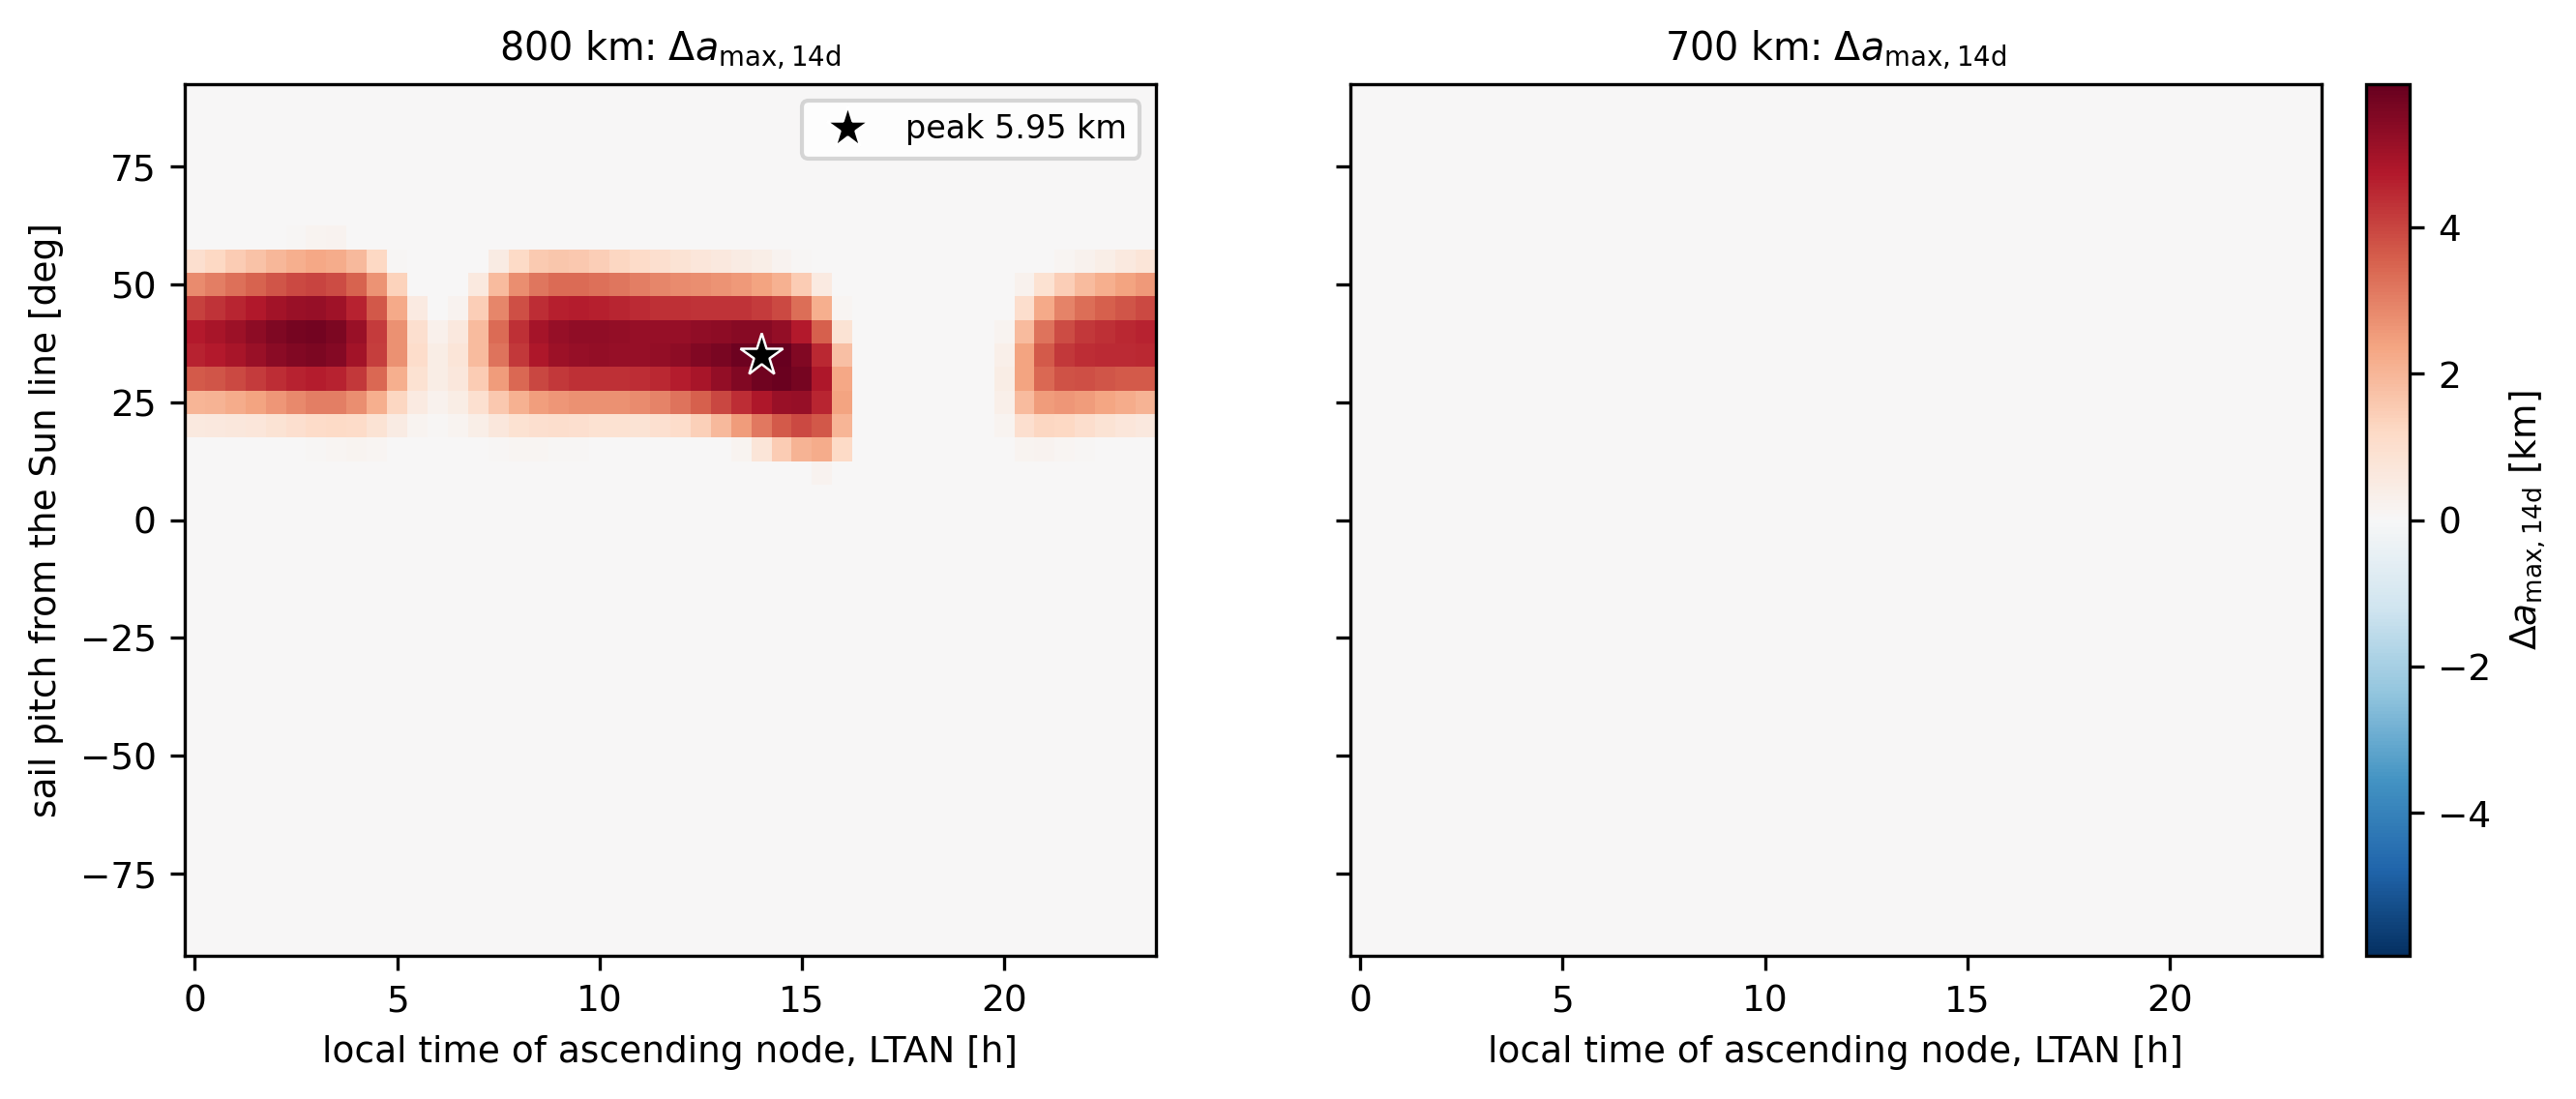
\includegraphics[width=1\linewidth]{Figures/r_map_ltan_pitch.png}
    \setlength{\abovecaptionskip}{0pt}
    \caption{Maximum \(14\)-day excursion of the mean semi-major axis, \(\Delta a_{\max,14\mathrm{d}}\), as a function of LTAN and initial sail pitch at \(800\,\mathrm{km}\) (left) and \(700\,\mathrm{km}\) (right); \(48\times37 = 1776\) cells per altitude, RK4 at \(10\,\mathrm{s}\), epoch 1 Jan 2026 12:00 UTC, baseline sail of Table~\ref{tab:baseline_params}. At \(800\,\mathrm{km}\) a single connected band of positive excursion occupies pitch \(+10^\circ\) to \(+60^\circ\) and LTAN \(20.0\,\mathrm{h}\) through midnight to \(16.0\,\mathrm{h}\), peaking at \(5.95\,\mathrm{km}\) at LTAN \(14.0\,\mathrm{h}\), pitch \(+35^\circ\) (star). At \(700\,\mathrm{km}\) no cell gains.}
    \label{fig:heatmap_700km}
\end{figure*}

\vspace{5pt}
\par\noindent At \(700\,\mathrm{km}\) the picture is qualitatively different: for the baseline atmosphere none of the \(1776\) cells shows a positive excursion within \(14\) days, so that \(\Delta a_{\max,14\mathrm{d}}\) vanishes over the whole map, the most negative \(14\)-day change is \(-62.05\,\mathrm{km}\), and the geometry that peaks at \(800\,\mathrm{km}\) gives \(\Delta a(14\,\mathrm{d}) = -13.75\,\mathrm{km}\). The regime is therefore geometry-selective, above all in the sign and magnitude of the pitch (only a sail tilted from the Sun line towards \(\hat{\mathbf{s}}_{\odot}\times\hat{\mathbf{h}}\) by \(10^\circ\) to \(60^\circ\) gains, and the mirror-image tilt always loses), and altitude-selective, since the SRP surplus that the eclipse makes available is worth some \(16\,\mathrm{km}\) in \(14\) days (the eclipse on/off separation of Figure~\ref{SMA_eclipse}) and is outweighed by drag \(100\,\mathrm{km}\) lower. The dependence on LTAN, by contrast, is considerably weaker than the original submission suggested: the band spans most of the LTAN circle, and the two ridge maxima differ by only \(0.2\,\mathrm{km}\).

\vspace{5pt}
\par\noindent Three representative \(800\,\mathrm{km}\) cases are used throughout the remainder of the paper and are collected, together with the former \(700\,\mathrm{km}\) anchor of the original submission, in Table~\ref{tab:cases}. The gain case is the peak cell of the map, LTAN \(14.0\,\mathrm{h}\) (RAAN \(312.05^\circ\) at epoch), pitch \(+35^\circ\); its \(14\)-day peak falls at day \(13.94\), the last ascending node of the window, so \(\Delta a_{\max,14\mathrm{d}} = \Delta a(14\,\mathrm{d}) = 5.95\,\mathrm{km}\) and the semi-major axis is still rising at day \(14\). The decay case is the most negative cell, LTAN \(0.0\,\mathrm{h}\) (RAAN \(102.05^\circ\)), pitch \(-30^\circ\). The neutral case, LTAN \(11.0\,\mathrm{h}\) (RAAN \(267.05^\circ\)), pitch \(+5^\circ\), is a nearly Sun-facing sail in a near-noon plane; it is the no-gain cell with \(|\mathrm{pitch}| \le 45^\circ\) whose \(14\)-day change, \(-9.885\,\mathrm{km}\), lies closest to the drag-only reference decay of \(-9.855\,\mathrm{km}\). Over \(75\) days only the gain case ever rises above \(a_0\); the neutral case ends at \(-150.9\,\mathrm{km}\), its nearly Sun-facing attitude also presenting a larger projected area to the flow, and the decay case and the former \(700\,\mathrm{km}\) anchor re-enter. These cases are used to separate bounded existence from mechanism.

\begin{table*}[htbp]
\centering
\caption{Representative cases used in Sections~\ref{sec:existence}--\ref{sec:validation}; the former anchor is the \(700\,\mathrm{km}\) geometry of the original submission. Epoch 1 Jan 2026 12:00 UTC; inclination \(98.31^\circ\) (\(800\,\mathrm{km}\)) and \(98.17^\circ\) (\(700\,\mathrm{km}\)); \(e_0 = 10^{-4}\); \(A/m = 10\,\mathrm{m^2\,kg^{-1}}\); \(C_r = 1.7\); \(C_D = 2.2\); RK4 at \(10\,\mathrm{s}\). RAAN is the epoch value corresponding to the stated LTAN (the original submission quoted the former anchor with RAAN \(285.5^\circ\); \(286.04^\circ\) is the value implied by the LTAN convention of Section~\ref{sec:model} at the stated epoch). \(\Delta a_{\max,14\mathrm{d}}\) is the largest positive excursion of the mean semi-major axis within \(14\) days (zero if none), \(\Delta a(14\,\mathrm{d})\) the value at day \(14\), \(\Delta a_{\max,75\mathrm{d}}\) the largest positive excursion within \(75\) days with its day, and \(\Delta a_{75\mathrm{d}}\) the value at day \(75\), or the re-entry day when the perigee altitude falls below \(120\,\mathrm{km}\) before then. The \(14\)-day peak of the gain case occurs at day \(13.94\), the last ascending node of the window.}
\label{tab:cases}
\vspace{0.5em}
\footnotesize
\setlength{\tabcolsep}{2.5pt}
\begin{tabular}{l c c c c c c c c}
\toprule
Case
& \begin{tabular}[c]{@{}c@{}}Alt.\\{}[km]\end{tabular}
& \begin{tabular}[c]{@{}c@{}}LTAN\\{}[h]\end{tabular}
& \begin{tabular}[c]{@{}c@{}}Pitch\\{}[deg]\end{tabular}
& \begin{tabular}[c]{@{}c@{}}RAAN\\{}[deg]\end{tabular}
& \begin{tabular}[c]{@{}c@{}}\(\Delta a_{\max,14\mathrm{d}}\)\\{}[km]\end{tabular}
& \begin{tabular}[c]{@{}c@{}}\(\Delta a(14\,\mathrm{d})\)\\{}[km]\end{tabular}
& \begin{tabular}[c]{@{}c@{}}\(\Delta a_{\max,75\mathrm{d}}\)\\{}[km]\end{tabular}
& \begin{tabular}[c]{@{}c@{}}\(\Delta a_{75\mathrm{d}}\)\\{}[km]\end{tabular} \\
\midrule
Gain & 800 & 14.0 & \(+35\) & 312.05 & 5.95 & \(+5.95\) & \begin{tabular}[c]{@{}c@{}}\(+10.86\)\\day 38.1\end{tabular} & \(-2.69\) \\
Neutral & 800 & 11.0 & \(+5\) & 267.05 & 0 & \(-9.89\) & 0 & \(-150.9\) \\
Decay & 800 & 0.0 & \(-30\) & 102.05 & 0 & \(-29.40\) & 0 & \begin{tabular}[c]{@{}c@{}}re-entry\\day 64.4\end{tabular} \\
Former anchor & 700 & 12.266 & \(+24.8\) & 286.04 & 0 & \(-21.07\) & 0 & \begin{tabular}[c]{@{}c@{}}re-entry\\day 39.5\end{tabular} \\
\bottomrule
\end{tabular}
\end{table*}

\vspace{5pt}
\par\noindent The most direct causal test is to compare the gain case with and without eclipse while holding every other initial condition and model assumption fixed. Figure~\ref{SMA_eclipse} shows that the short-horizon outcome reverses under that single change. By day \(14\) the eclipse-on case reaches \(\Delta a(14\,\mathrm{d}) = +5.95\,\mathrm{km}\), whereas the eclipse-off counterpart has fallen to \(-10.59\,\mathrm{km}\), a separation of \(16.5\,\mathrm{km}\). The eclipse-off value lies within \(0.7\,\mathrm{km}\) of the drag-only run of the same geometry (\(-9.89\,\mathrm{km}\)): with the umbra removed, SRP contributes essentially nothing over \(14\) days, because the orbit-averaged SRP work of a fixed-attitude sail under continuous illumination cancels, exactly as the symmetry argument of Section~\ref{sec:physics} (Eq.~\eqref{eq:full_cancellation}) requires. At the former \(700\,\mathrm{km}\) anchor (right panel) the values are \(-21.07\,\mathrm{km}\) with eclipse on and \(-45.36\,\mathrm{km}\) with it off: the eclipse still removes the unfavourable arc, worth \(24.3\,\mathrm{km}\) over \(14\) days, but at this altitude drag wins regardless. Over \(75\) days the eclipse-on gain case ends at \(-2.69\,\mathrm{km}\) and the eclipse-off counterpart at \(-110.5\,\mathrm{km}\) (Section~\ref{sec:breakdown}). The gain case is therefore not SRP-favourable in a generic sense; its transient improvement depends on eclipse.

\begin{figure*}[htbp]
    \centering
    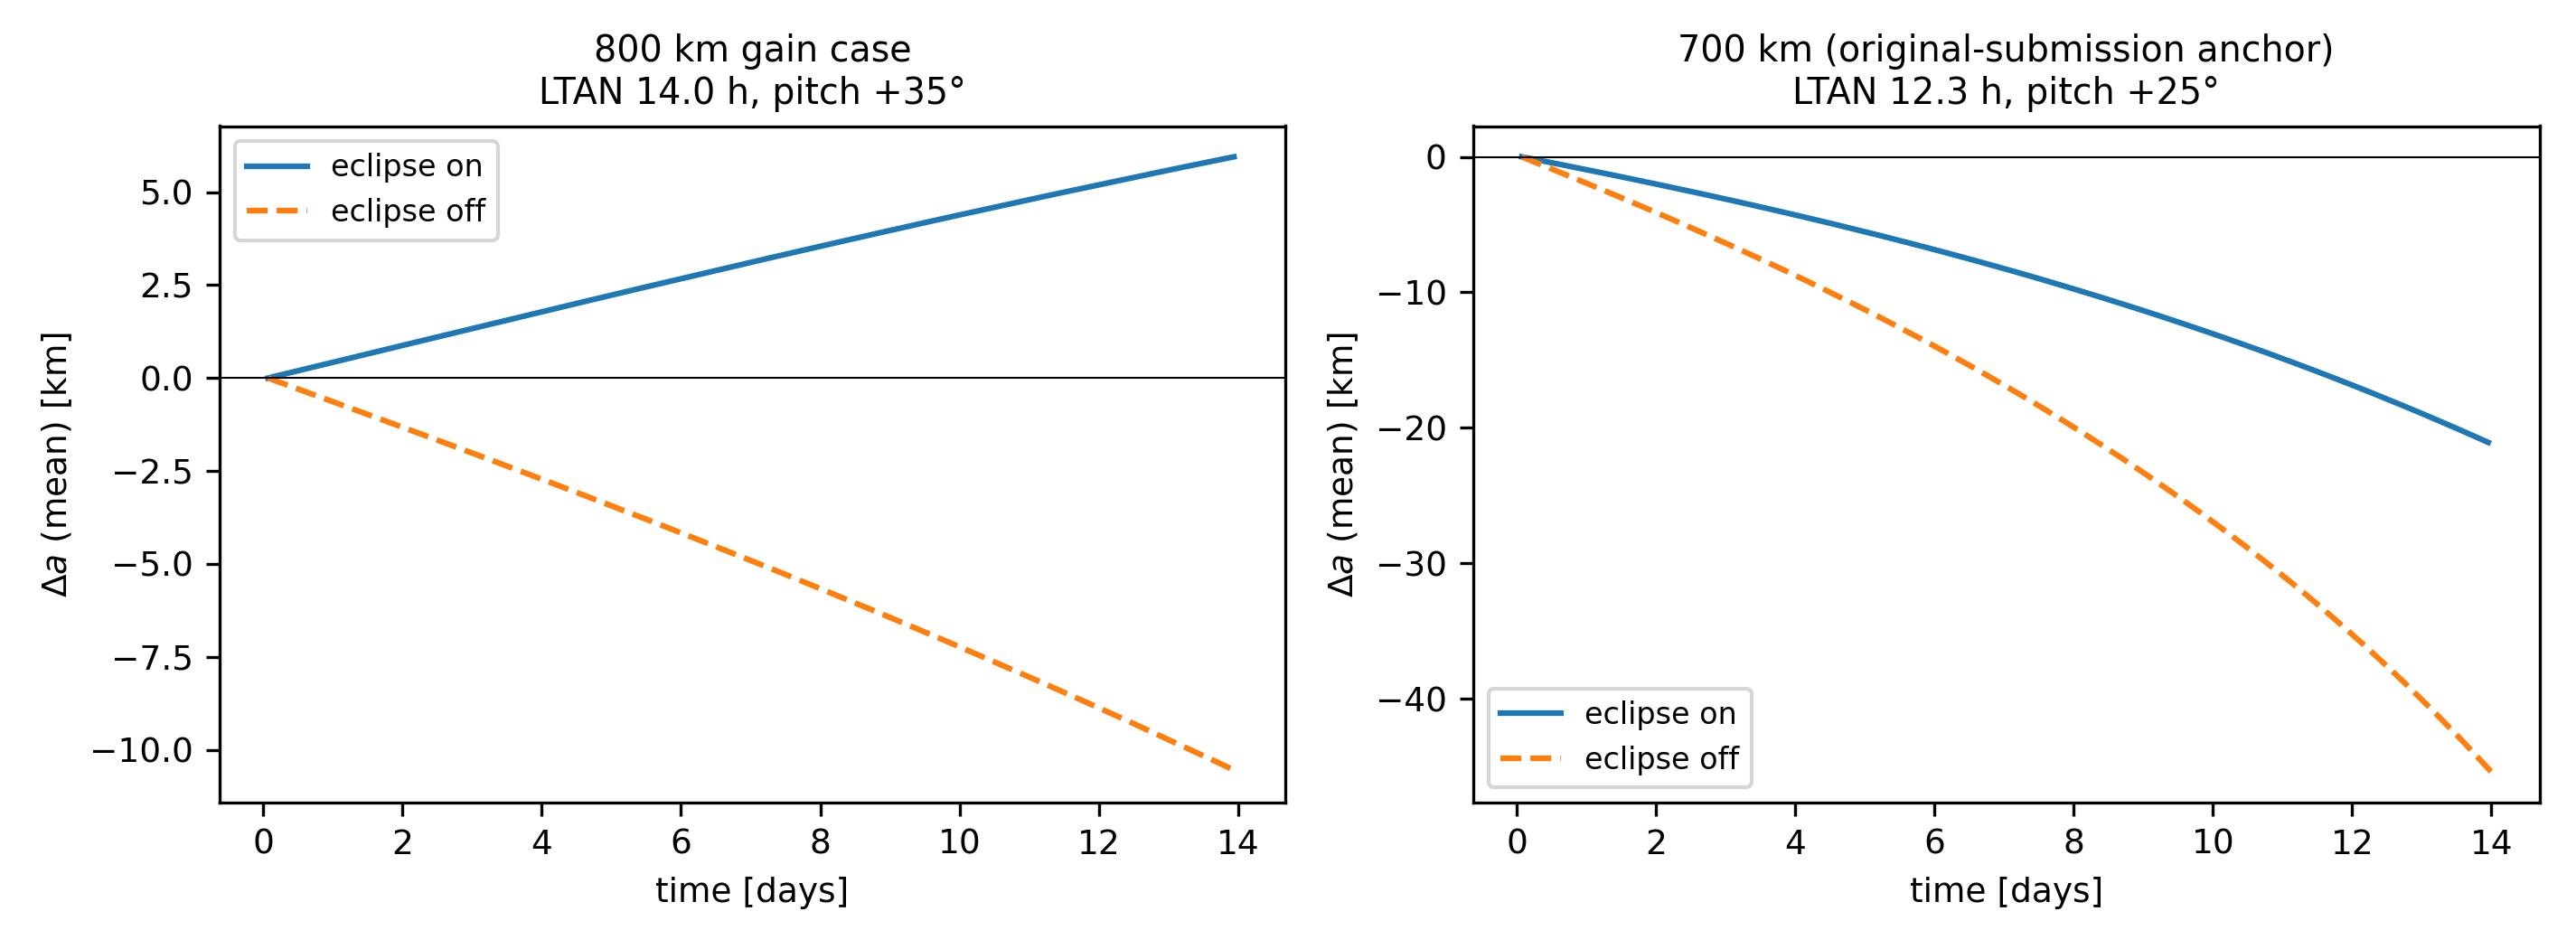
\includegraphics[width=1\linewidth]{Figures/r_eclipse_onoff.png}
    \setlength{\abovecaptionskip}{0pt}
    \caption{Mean semi-major-axis change over \(14\) days with eclipse on and off, all other conditions fixed. Left: the \(800\,\mathrm{km}\) gain case (LTAN \(14.0\,\mathrm{h}\), pitch \(+35^\circ\)), \(+5.95\,\mathrm{km}\) with eclipse on against \(-10.59\,\mathrm{km}\) with it off. Right: the former \(700\,\mathrm{km}\) anchor (LTAN \(12.266\,\mathrm{h}\), pitch \(+24.8^\circ\)), \(-21.07\) against \(-45.36\,\mathrm{km}\).}
    \label{SMA_eclipse}
\end{figure*}

\vspace{5pt}
\par\noindent A second control isolates which component of the SRP force carries the effect. Repeating the gain case with eclipse on but with the whole SRP force directed along the Sun line instead of the plate normal gives \(\Delta a_{\max,14\mathrm{d}} = 0\) and \(\Delta a(14\,\mathrm{d}) = -10.50\,\mathrm{km}\): no gain at all, and marginally worse than with SRP switched off (\(-9.89\,\mathrm{km}\)), because a force of fixed inertial direction along the Sun line performs no net orbit-averaged work in this geometry yet still pumps the eccentricity, exposing the perigee to slightly more drag. This confirms numerically the statement of Sections~\ref{sec:physics} and \ref{sec:model} that the along-normal (specular) component carries the eclipse-gated mechanism.

\vspace{5pt}
\par\noindent The eclipse-on/off comparison establishes causality but not the orbit-scale mechanism. Figure~\ref{srp_vs_anomaly} addresses that by plotting the instantaneous SRP specific power, \(\mathbf{a}_{\mathrm{SRP}}\!\cdot\!\mathbf{v}\), against time from the ascending node over one node-to-node orbit at epoch (nodal period \(100.8\,\mathrm{min}\) in all three cases, sampled at \(2\,\mathrm{s}\)) for the gain, neutral and decay cases, with the umbra shaded and the no-eclipse reference dashed. In the gain case the umbra occupies \(32.1\%\) of the orbit and falls predominantly on the arc where the normal-directed force would decelerate the sail: \(77.4\%\) of the eclipsed samples correspond to negative no-eclipse SRP power, and by integrated magnitude the shadow suppresses \(-344.2\,\mathrm{J\,kg^{-1}}\) of harmful work while removing only \(+35.3\,\mathrm{J\,kg^{-1}}\) of beneficial work. In the decay case the umbra fraction is \(34.9\%\) but only \(30.7\%\) of the eclipsed samples are negative: the shadow now covers the accelerating arc, suppressing \(+410.2\,\mathrm{J\,kg^{-1}}\) of beneficial work against \(-94.4\,\mathrm{J\,kg^{-1}}\) of harmful work. In the neutral case (umbra fraction \(34.6\%\)) the SRP power is close to antisymmetric about the umbra, so the shadow removes nearly equal shares of each sign (\(53.3\%\) of eclipsed samples negative; suppressed work \(-337.4\) against \(+264.9\,\mathrm{J\,kg^{-1}}\)) and eclipse changes little. The mechanism is therefore sign-selective: the outcome depends on which branch of the SRP-power cycle the shadow removes, which is set by the orientation of the umbra relative to the fixed sail normal, i.e.\ by LTAN and pitch together.

\begin{figure*}[htbp]
    \centering
    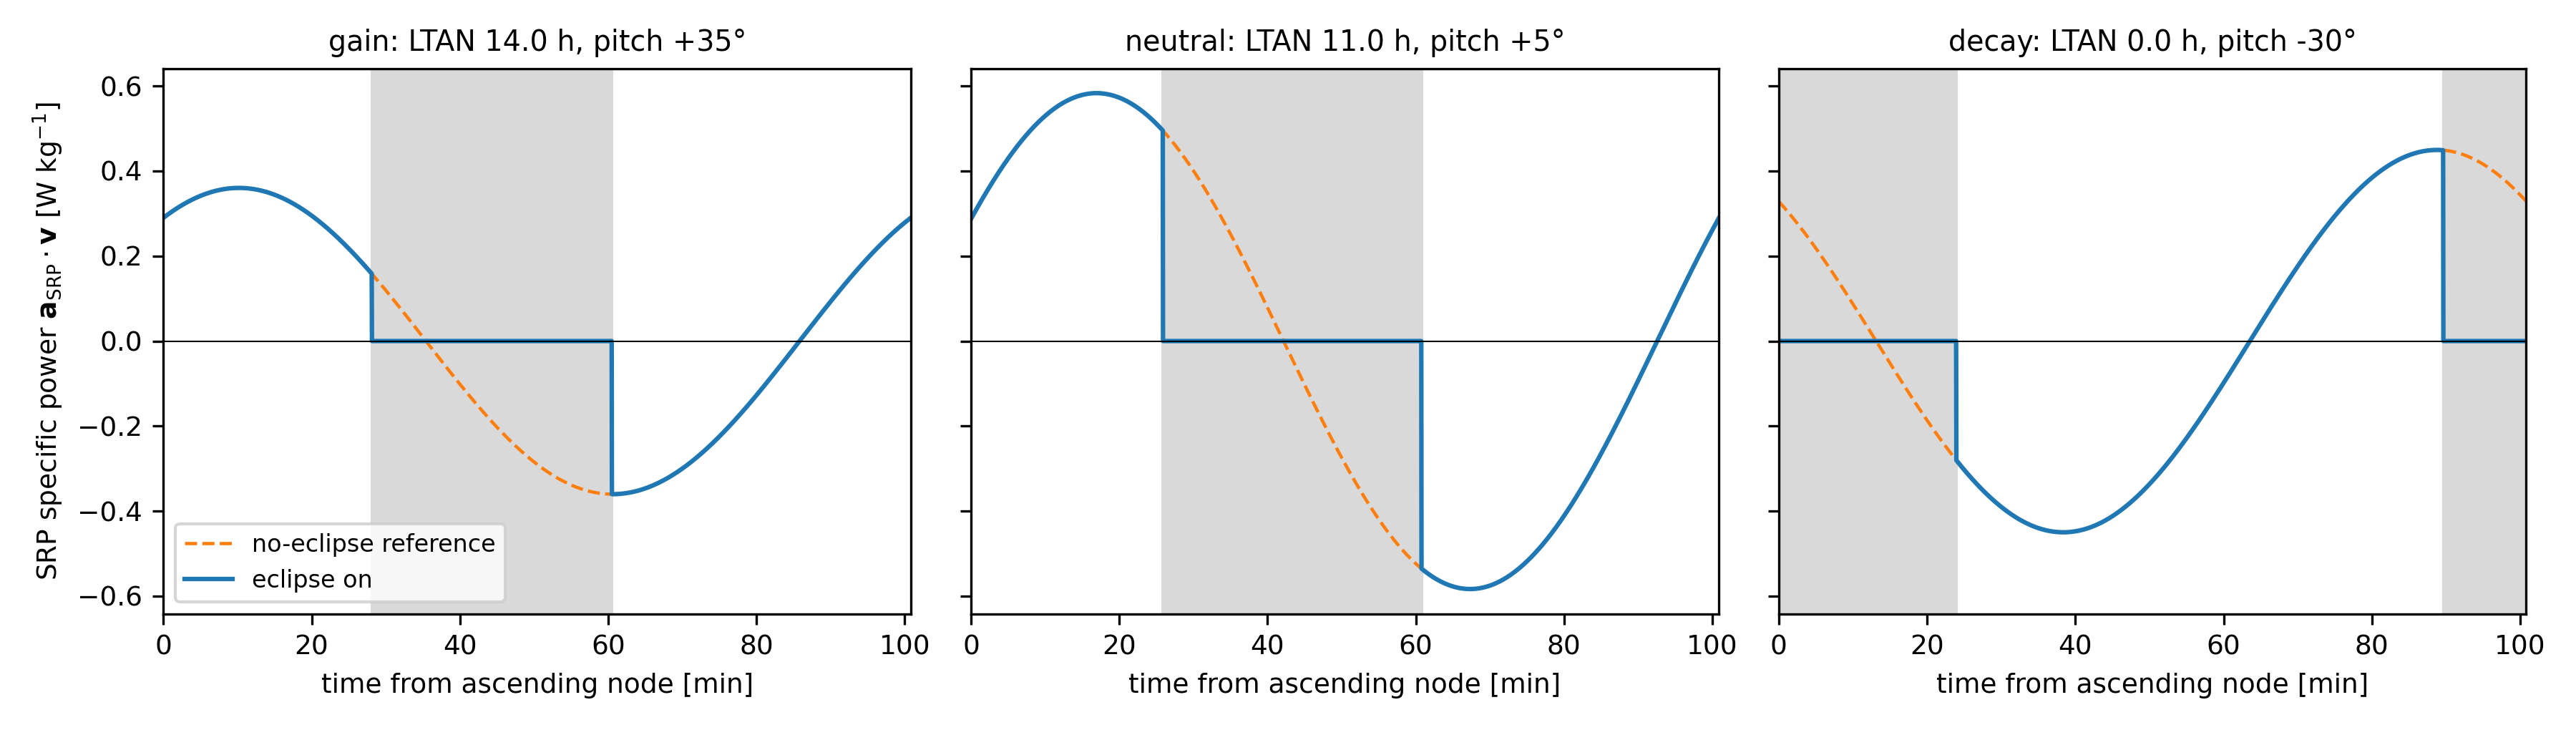
\includegraphics[width=1\linewidth]{Figures/r_srp_power.png}
    \setlength{\abovecaptionskip}{0pt}
    \caption{Instantaneous SRP specific power, \(\mathbf{a}_{\mathrm{SRP}}\!\cdot\!\mathbf{v}\), against time from the ascending node over one node-to-node orbit at epoch (nodal period \(100.8\,\mathrm{min}\)) for the \(800\,\mathrm{km}\) gain, neutral and decay cases of Table~\ref{tab:cases}. Shading marks the umbra; the dashed curve is the no-eclipse reference. The shadow suppresses a predominantly negative-power arc in the gain case (\(77.4\%\) of eclipsed samples negative), a predominantly positive-power arc in the decay case (\(30.7\%\)), and nearly equal shares in the neutral case (\(53.3\%\)).}
    \label{srp_vs_anomaly}
\end{figure*}

\vspace{5pt}
\par\noindent Figure~\ref{cum_SRP} shows the same effect in cumulative form. With eclipse off, the cumulative SRP specific work over the orbit is near zero in every geometry, \(+1.4\), \(+0.9\) and \(+0.4\,\mathrm{J\,kg^{-1}}\) for the gain, neutral and decay cases: this is the passive cancellation of Section~\ref{sec:physics}, and it holds irrespective of LTAN and pitch. With eclipse on, the orbit closes at \(+310.3\,\mathrm{J\,kg^{-1}}\) in the gain geometry, \(+73.5\,\mathrm{J\,kg^{-1}}\) in the neutral geometry (a quarter of the gain value) and \(-315.4\,\mathrm{J\,kg^{-1}}\) in the decay geometry. Eclipse timing therefore sets the \emph{sign} of the orbit-averaged SRP work, not merely its magnitude. The Sun-line variant of the gain case (dotted curve in the gain panel) closes at \(+1.0\,\mathrm{J\,kg^{-1}}\) with eclipse on, indistinguishable from the no-eclipse reference: this is the one-orbit counterpart of the \(14\)-day Sun-line result above. The shadow thus converts a cancelling SRP work cycle into a net surplus only in the gain geometry, into a net deficit in the decay geometry, and in the neutral geometry leaves a small residual that drag swamps.

\begin{figure*}[htbp]
    \centering
    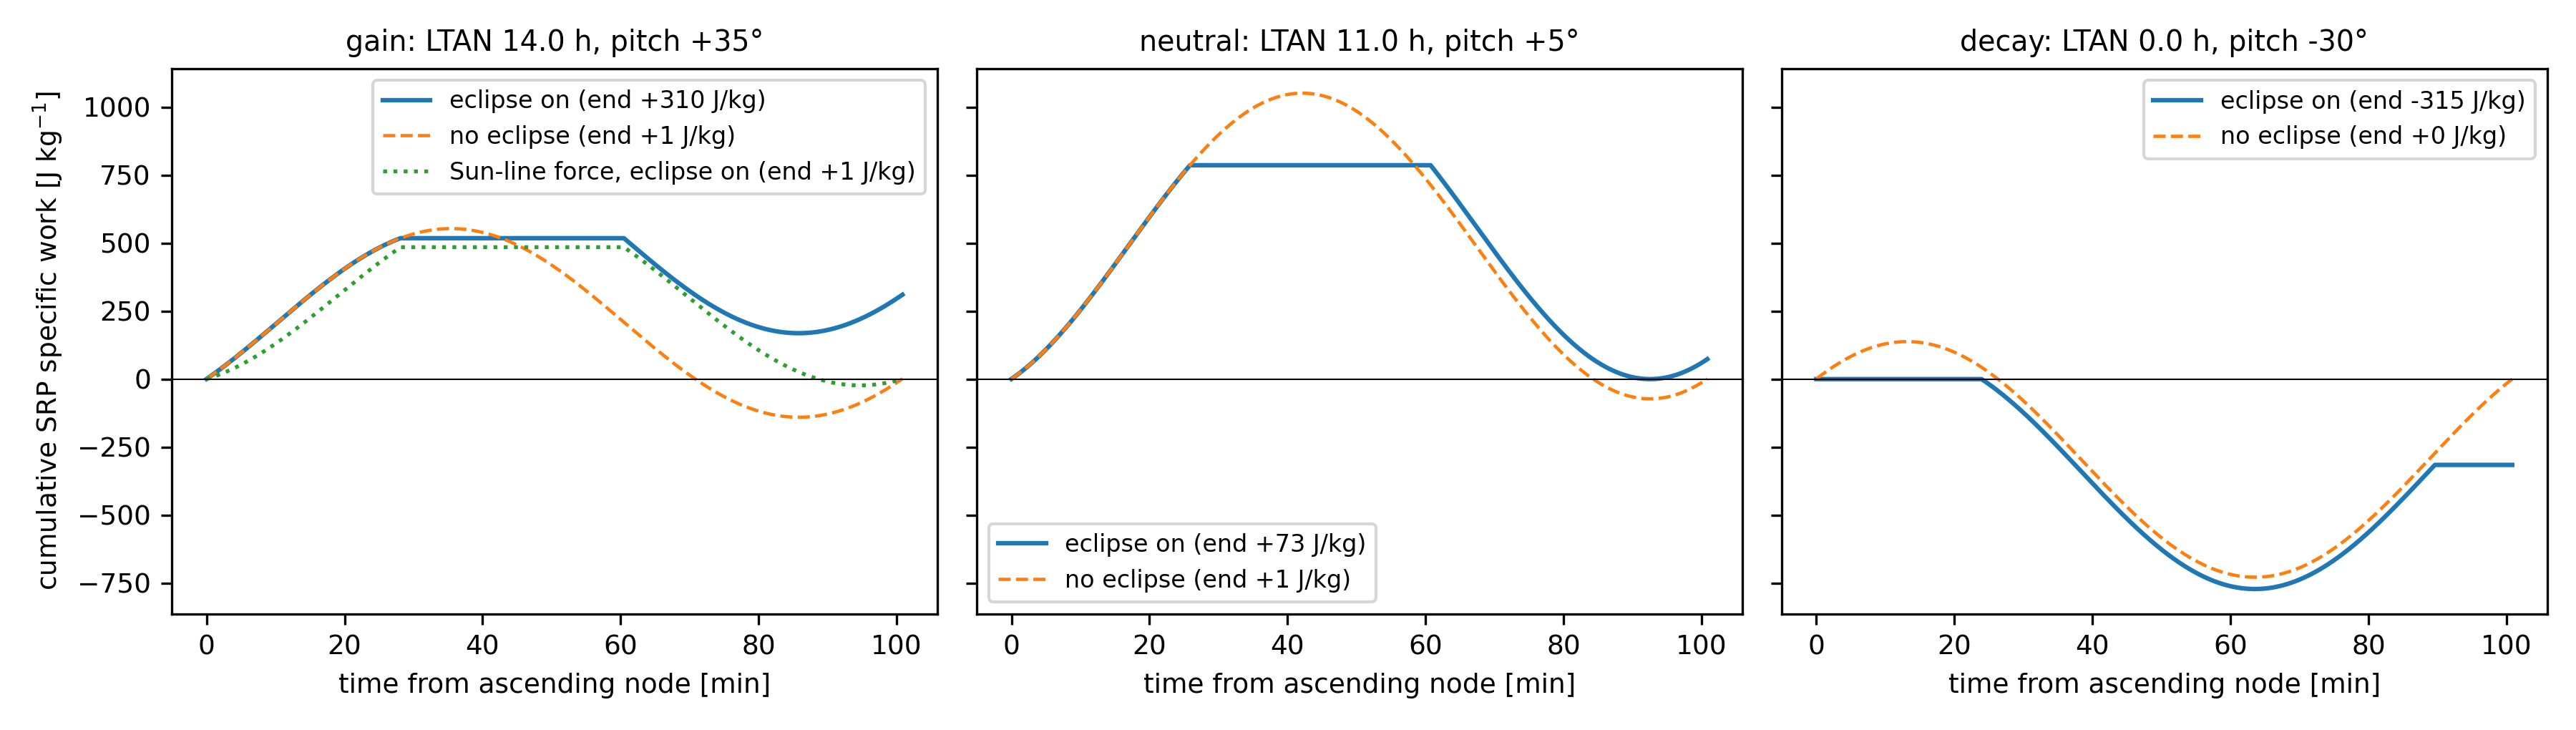
\includegraphics[width=1\linewidth]{Figures/r_cum_srp_work.png}
    \setlength{\abovecaptionskip}{0pt}
    \caption{Cumulative SRP specific work over the same node-to-node orbit as Figure~\ref{srp_vs_anomaly} for the gain, neutral and decay cases, with eclipse on (solid) and the no-eclipse reference (dashed). The eclipse-on end values are \(+310.3\), \(+73.5\) and \(-315.4\,\mathrm{J\,kg^{-1}}\); the no-eclipse references end at \(+1.4\), \(+0.9\) and \(+0.4\,\mathrm{J\,kg^{-1}}\). The dotted curve in the gain panel is the Sun-line force variant with eclipse on, ending at \(+1.0\,\mathrm{J\,kg^{-1}}\).}
    \label{cum_SRP}
\end{figure*}

\vspace{5pt}
\par\noindent Taken together, the results in this section establish three points. First, a bounded transient-gain region exists at \(800\,\mathrm{km}\) in LTAN--pitch space, confined to positive pitch between \(+10^\circ\) and \(+60^\circ\) and peaking at \(5.95\,\mathrm{km}\) in \(14\) days, while the same sail gains nowhere at \(700\,\mathrm{km}\). Second, eclipse is causally decisive: removing the umbra at the gain geometry turns \(+5.95\,\mathrm{km}\) into \(-10.59\,\mathrm{km}\), within \(0.7\,\mathrm{km}\) of the drag-only outcome of \(-9.89\,\mathrm{km}\). Third, the mechanism is sign-selective: under continuous illumination the one-orbit SRP work cancels in every geometry, and the shadow helps only when it removes the negative-power branch of the cycle; the along-normal force component carries the effect, and a Sun-line force of the same magnitude produces none. The gain is nonetheless transient. The \(5.95\,\mathrm{km}\) attained within \(14\) days grows to \(+10.86\,\mathrm{km}\) by day \(38.1\), but this is not clean or sustained whole-orbit raising: by day \(75\) the mean semi-major axis has fallen back to \(-2.69\,\mathrm{km}\), through apogee pumping with perigee erosion and the drift of the inertially fixed sail normal away from the Sun line, as Section~\ref{sec:breakdown} shows. Nor is the regime an artefact of this implementation: at the gain anchor STK Astrogator gives \(+6.44\,\mathrm{km}\) with eclipse on and \(-10.13\,\mathrm{km}\) with it off over \(14\) days, against \(+5.85\) and \(-10.93\,\mathrm{km}\) for the present propagator under the centred one-period-mean definition used in that comparison, and Orekit gives \(+6.13\,\mathrm{km}\) against \(+5.93\,\mathrm{km}\) for the same case at a common \(30\,\mathrm{s}\) step (Section~\ref{sec:validation}).

\FloatBarrier


\section{Coupled Orbital Evolution and Breakdown of the Gain Regime}
\label{sec:breakdown}
\FloatBarrier
\noindent The representative gain trajectory must now be examined over a longer horizon to determine what the early increase in semi-major axis actually corresponds to dynamically, and why that favourable behaviour does not persist. The central result is simple to state: the early increase in \(a\) is real, but it is produced mainly by apogee pumping rather than by a clean upward translation of the whole orbit. This increases eccentricity, lowers perigee and concentrates drag loss near perigee; at the same time the inertially fixed sail normal drifts steadily out of alignment with the Sun, so that the SRP forcing which created the gain collapses in magnitude. The second of these effects dominates the late-time behaviour. Together they drive the orbit-averaged energy balance negative at the peak of \(a\), and by day \(75\) the accumulated surplus has been fully erased.

\vspace{5pt}
\par\noindent Figure~\ref{fig:elementsvstime} makes the first part of that breakdown visible directly. For the representative \(800\,\mathrm{km}\) gain case introduced in Section~\ref{sec:existence} (LTAN \(14.0\,\mathrm{h}\), pitch \(+35^\circ\), RAAN \(312.05^\circ\)), the \(75\)-day histories of mean \(a\), apogee altitude, perigee altitude and eccentricity show that the orbit is not lifted uniformly. Apogee grows far more than perigee is preserved, so the early gain develops together with a progressive departure from circularity. The neutral and decay cases are overlaid for comparison: the decay case (LTAN \(0.0\,\mathrm{h}\), pitch \(-30^\circ\)) loses altitude monotonically and re-enters on day \(64.4\), while the neutral case follows an intermediate, drag-like path between the two. Table~\ref{tab:gaincase_longhorizon_summary} collects the corresponding quantities for the gain case.

\begin{table*}[htbp]
\centering
\caption{Long-horizon summary of the representative \(800\,\mathrm{km}\) gain case over the \(75\)-day propagation (\(1069\) orbits). The case corresponds to altitude \(800\,\mathrm{km}\), LTAN \(14.0\,\mathrm{h}\) (RAAN \(312.05^\circ\)), pitch \(+35^\circ\), inclination \(98.31^\circ\), \(e_0=10^{-4}\), sail area \(100\,\mathrm{m^2}\), mass \(m=10\,\mathrm{kg}\), \(C_r=1.7\) and \(C_D=2.2\). Mean (secular) elements are osculating values sampled at ascending-node crossings. All work quantities are specific, i.e. per unit mass (\(m=10\,\mathrm{kg}\)).}
\label{tab:gaincase_longhorizon_summary}
\small
\begin{tabular}{p{4.9cm} p{1.8cm} p{3.2cm} p{1.8cm}}
\toprule
Quantity & Initial & Peak / minimum (day) & Final (day \(75\)) \\
\midrule
Mean semi-major axis, \(a\) [km]
& 7178.168
& 7189.030 (max, day 38.1)
& 7175.479 \\

Peak excursion, \(\Delta a_{\max,75\mathrm{d}}\) [km]
& \multicolumn{3}{l}{\(+10.86\) (day 38.1)} \\

Net change, \(\Delta a_{75\mathrm{d}}\) [km]
& \multicolumn{3}{l}{\(-2.69\)} \\

Apogee altitude [km]
& 801.0
& 912.0 (max, day 43.9)
& 884.7 \\

Perigee altitude [km]
& 799.1
& 708.6 (min, day 48.4)
& 709.9 \\

Eccentricity, \(e\)
& \(1.35\times10^{-4}\)
& \(1.41\times10^{-2}\) (max, day 45.2)
& \(1.22\times10^{-2}\) \\

Cumulative SRP work at day 75 [kJ\,kg\(^{-1}\)]
& \multicolumn{3}{l}{\(+194.5\)} \\

Cumulative drag work at day 75 [kJ\,kg\(^{-1}\)]
& \multicolumn{3}{l}{\(-204.4\)} \\

Cumulative total work at day 75 [kJ\,kg\(^{-1}\)]
& \multicolumn{3}{l}{\(-9.9\)} \\

Work ratio at day 75, \(\left|W_{\mathrm{drag}}\right|/\left|W_{\mathrm{SRP}}\right|\)
& \multicolumn{3}{l}{1.051} \\
\bottomrule
\end{tabular}
\end{table*}

\begin{figure*}[htbp]
    \centering
    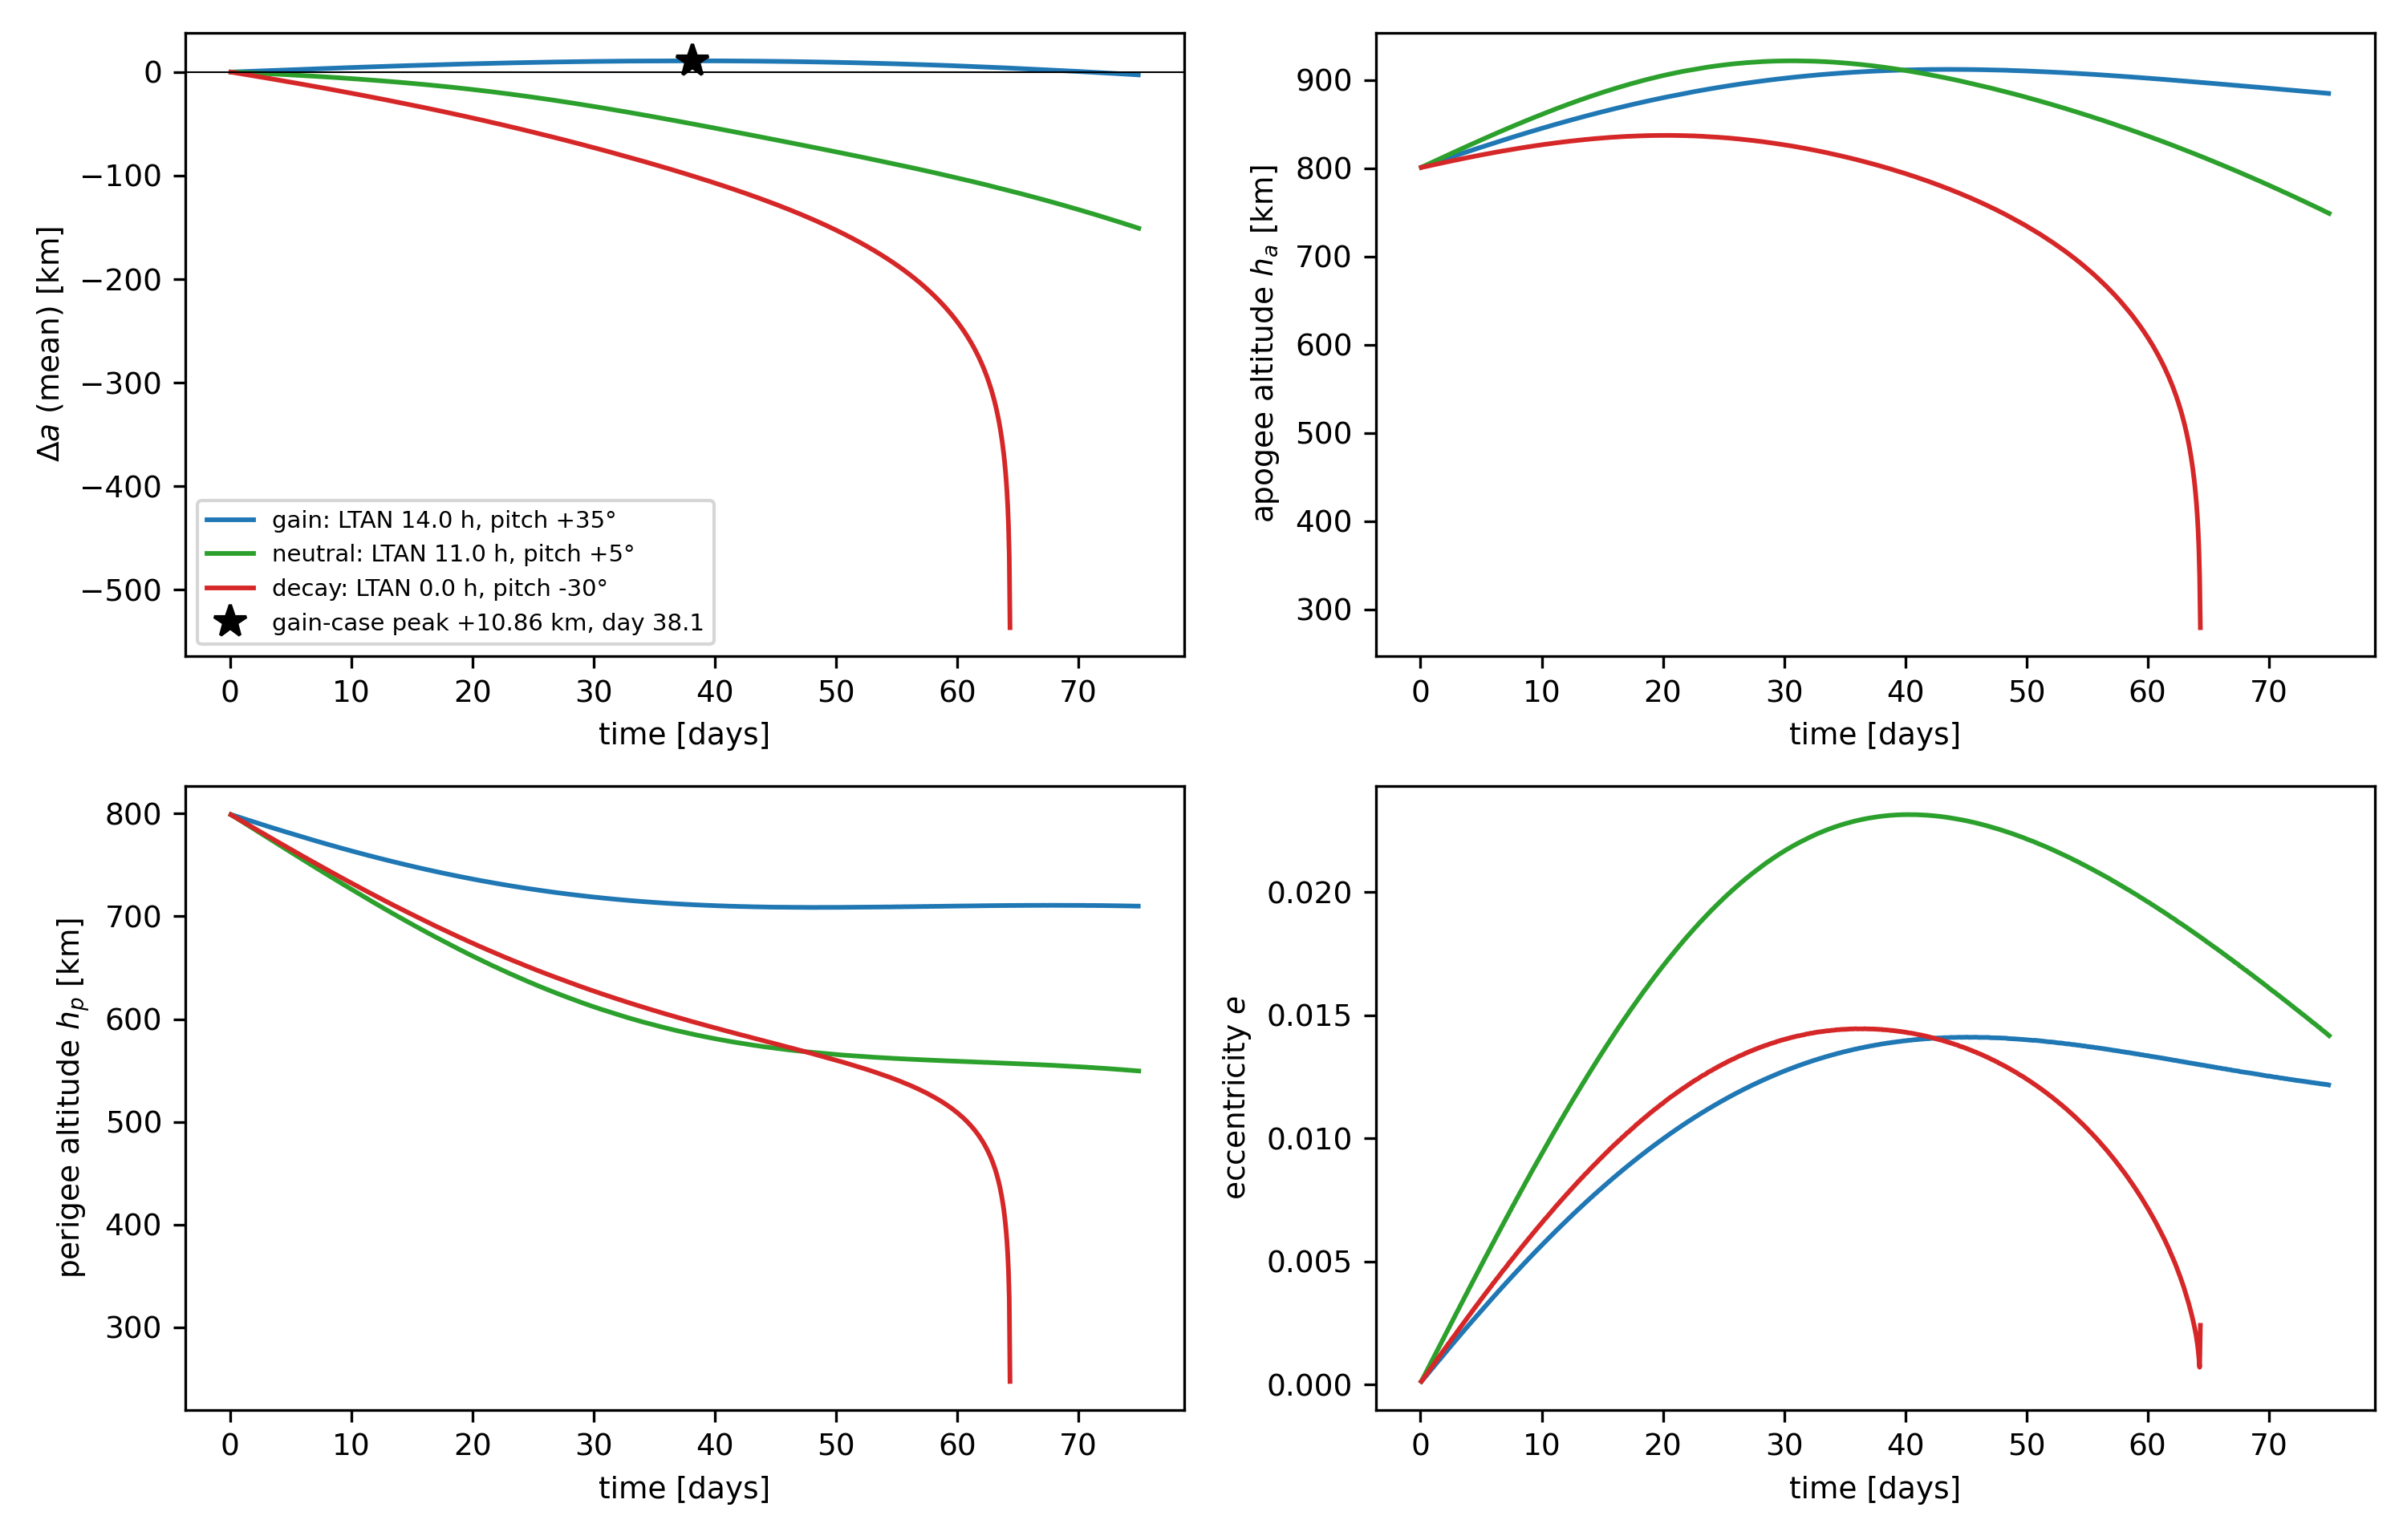
\includegraphics[width=1\linewidth]{Figures/r_elements_75d.png}
    \setlength{\abovecaptionskip}{0pt}
    \caption{Long-horizon evolution of mean orbital elements over \(75\) days for the representative \(800\,\mathrm{km}\) gain, neutral and decay cases: change in mean semi-major axis \(\Delta a\) (with the gain-case peak marked), apogee altitude, perigee altitude and eccentricity. The gain case shows non-monotonic semi-major-axis evolution, strong apogee growth, perigee erosion and eccentricity growth; the decay case re-enters on day \(64.4\).}
    \label{fig:elementsvstime}
\end{figure*}

\vspace{5pt}
\par\noindent The mean semi-major axis of the gain case begins at \(a_0 = 7178.168\,\mathrm{km}\), rises to \(\Delta a(14\,\mathrm{d}) = +5.95\,\mathrm{km}\) at the last ascending node of the \(14\)-day window (day \(13.94\); this is the same trajectory, and the same value, that anchors Section~\ref{sec:existence}), and continues upward more slowly: \(+9.96\,\mathrm{km}\) on day \(28\) and a peak of \(\Delta a_{\max,75\mathrm{d}} = +10.86\,\mathrm{km}\) (\(a = 7189.030\,\mathrm{km}\)) on day \(38.1\). It then declines for the remainder of the propagation, passing \(+10.70\,\mathrm{km}\) on day \(42\), \(+7.59\,\mathrm{km}\) on day \(56\) and \(+0.59\,\mathrm{km}\) on day \(70\), returning to its initial value on day \(71.0\) and finishing at \(\Delta a_{75\mathrm{d}} = -2.69\,\mathrm{km}\) (\(a = 7175.479\,\mathrm{km}\)). The behaviour is therefore explicitly non-monotonic: there is a finite interval of positive excursion lasting roughly ten weeks, but not sustained orbit raising. The short-horizon gain is real, yet by the end of the \(75\)-day window it has been entirely given back.

\vspace{5pt}
\par\noindent The apogee--perigee split shows how that reversal develops. Apogee altitude rises from \(801.0\,\mathrm{km}\) to \(860.4\,\mathrm{km}\) by day \(14\) and \(910.4\,\mathrm{km}\) by day \(38\), peaks at \(912.0\,\mathrm{km}\) on day \(43.9\), and is still \(884.7\,\mathrm{km}\) at day \(75\). Perigee altitude falls from \(799.1\,\mathrm{km}\) to \(751.6\,\mathrm{km}\) by day \(14\) and \(711.3\,\mathrm{km}\) by day \(38\), reaches its minimum of \(708.6\,\mathrm{km}\) on day \(48.4\), and remains depressed at \(709.9\,\mathrm{km}\) at day \(75\). The eccentricity correspondingly grows from \(1.35\times10^{-4}\) to a maximum of \(1.41\times10^{-2}\) on day \(45.2\) and relaxes only slightly to \(1.22\times10^{-2}\). The key point is geometric rather than merely descriptive: the \(+10.86\,\mathrm{km}\) peak in \(a\) is achieved by stretching the orbit, with apogee raised by over \(100\,\mathrm{km}\) while perigee is lowered by about \(90\,\mathrm{km}\), not by lifting it uniformly.

\vspace{5pt}
\par\noindent The physical consequence is that drag loss becomes progressively concentrated near perigee, where the atmosphere is densest. This is the first breakdown pathway visible in the long-horizon outputs: the same evolution that produces the early gain also creates a lower-perigee, more eccentric orbit that is increasingly exposed to atmospheric loss. Eclipse remains essential throughout. Repeating the gain case with the umbra disabled, so that SRP acts around the whole orbit, gives \(\Delta a_{75\mathrm{d}} = -110.5\,\mathrm{km}\), a perigee minimum of \(592.7\,\mathrm{km}\) and \(e_{\max} = 0.0189\): without the eclipse-induced sign selectivity of Section~\ref{sec:existence} the same attitude pumps eccentricity even harder while contributing essentially no net energy, and the orbit ends \(108\,\mathrm{km}\) lower after \(75\) days. The decay case illustrates the same eccentricity pumping with the wrong sign of net work: its eccentricity reaches \(0.0145\) on day \(36.6\), and perigee erosion then runs away to re-entry on day \(64.4\). The former \(700\,\mathrm{km}\) configuration of the original submission (LTAN \(12.266\,\mathrm{h}\), pitch \(24.8^\circ\)) behaves likewise and re-enters on day \(39.5\).

\vspace{5pt}
\par\noindent The cumulative work budget in Figure~\ref{fig:gaincase_cumulative_work_budget} must be read carefully. Over the full \(75\)-day window the cumulative specific SRP work is \(+194.5\,\mathrm{kJ\,kg^{-1}}\) and the cumulative drag work is \(-204.4\,\mathrm{kJ\,kg^{-1}}\), so the cumulative total is \(-9.9\,\mathrm{kJ\,kg^{-1}}\) and \(|W_{\mathrm{drag}}|/|W_{\mathrm{SRP}}| = 1.051\). The total does not fall monotonically: it rises to a maximum of \(+41.3\,\mathrm{kJ\,kg^{-1}}\) on day \(38.1\), the same day on which mean \(a\) peaks, and then declines, crossing zero on day \(71.2\). This is consistent with the semi-major-axis history, since \(\Delta a \simeq (2a^2/\mu)\,W_{\mathrm{total}}\) gives \(-2.6\,\mathrm{km}\) for the day-\(75\) total, matching the node-sampled \(\Delta a_{75\mathrm{d}} = -2.69\,\mathrm{km}\) and the zero crossing of mean \(a\) on day \(71.0\). The regime therefore does more than stop strengthening at late times: the surplus accumulated during the favourable phase is unwound in full, and slightly overshot, within the analysed window.

\begin{figure}[htbp]
    \centering
    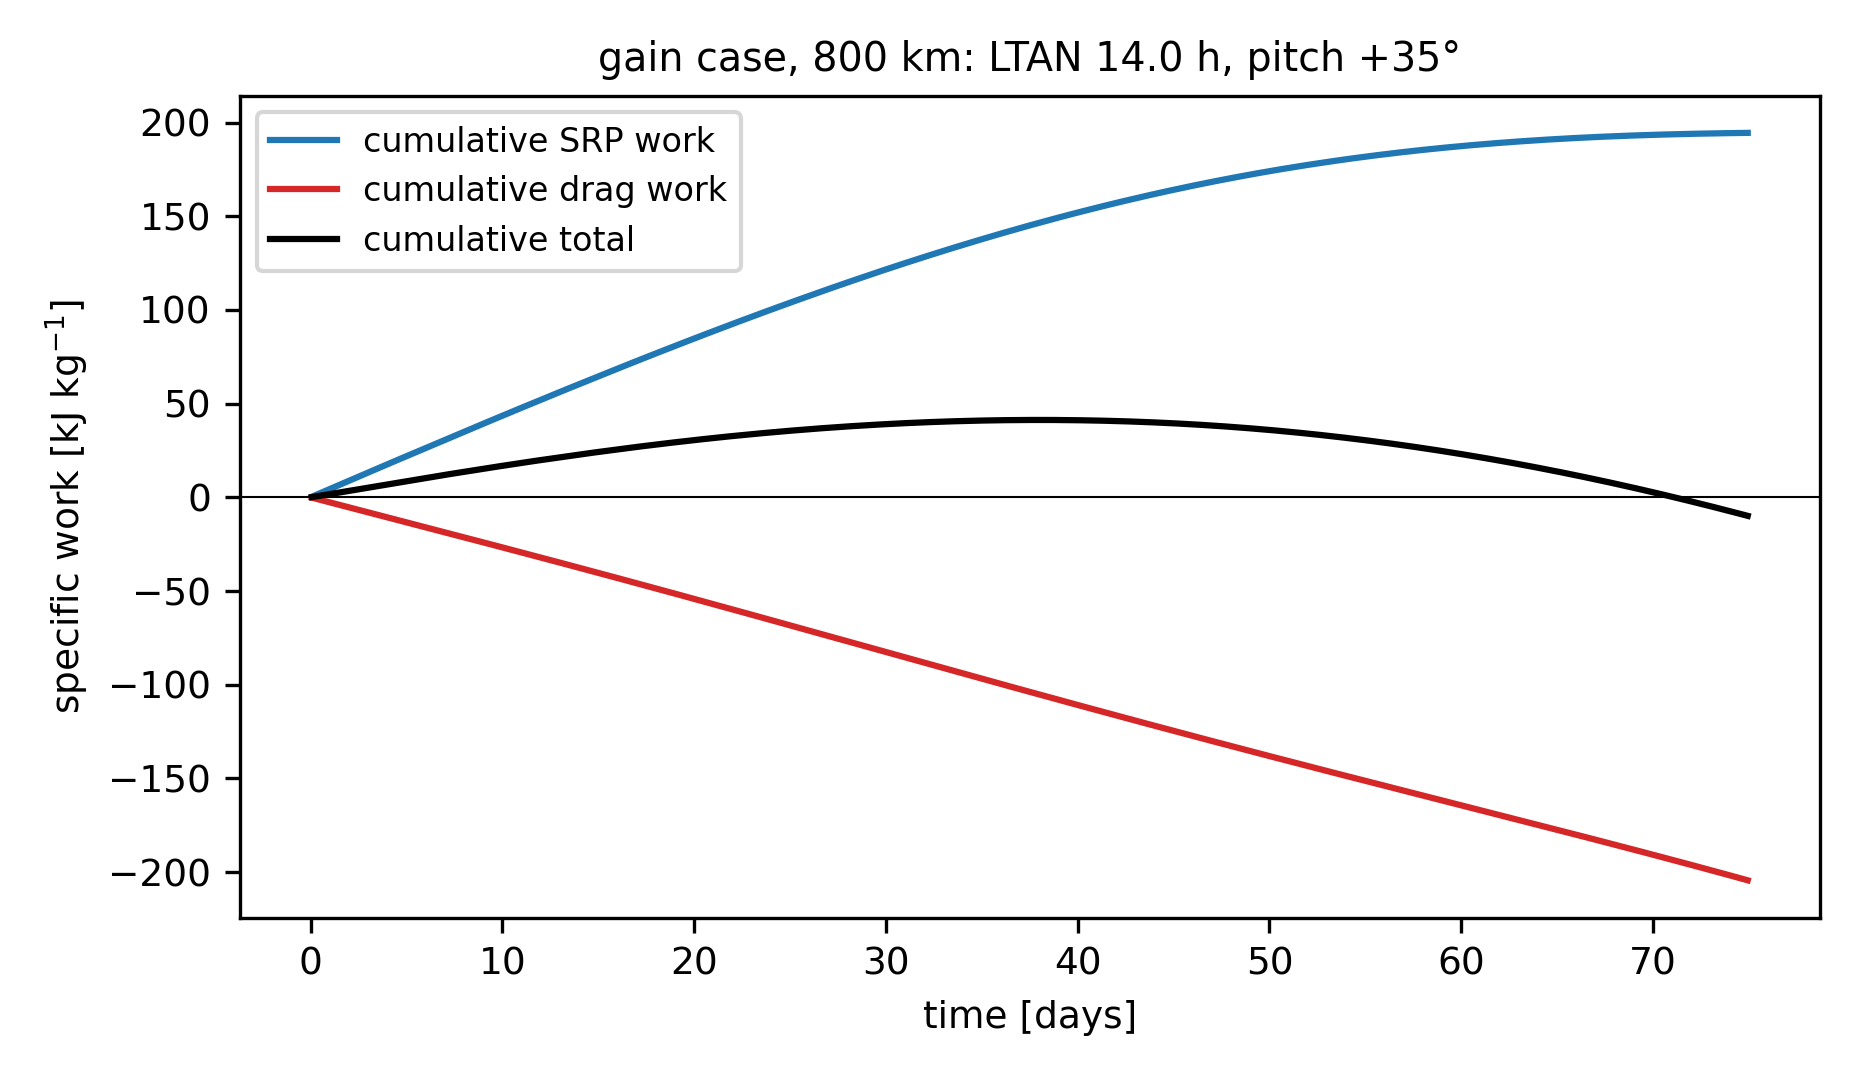
\includegraphics[width=0.8\linewidth]{Figures/r_cum_work_75d.png}
    \setlength{\abovecaptionskip}{0pt}
    \caption{Cumulative specific SRP work, drag work and total work (\(\mathrm{kJ\,kg^{-1}}\)) for the representative \(800\,\mathrm{km}\) gain case over \(75\) days. The cumulative total peaks at \(+41.3\,\mathrm{kJ\,kg^{-1}}\) on day \(38.1\) and turns negative on day \(71.2\); by day \(75\) cumulative drag exceeds cumulative SRP work by \(5.1\%\).}
    \label{fig:gaincase_cumulative_work_budget}
\end{figure}

\vspace{5pt}
\par\noindent The more revealing diagnostic is the orbit-averaged early-versus-late comparison in the left panel of Figure~\ref{fig:gaincase_early_late_work_comparison} and in Table~\ref{tab:gaincase_earlylate_comparison}, which compares the first and last \(20\%\) of the run (\(214\) of \(1069\) orbits each). Early in the run the mean SRP contribution of \(+301.3\,\mathrm{J\,kg^{-1}\,orbit^{-1}}\) exceeds the mean drag loss of \(-188.3\,\mathrm{J\,kg^{-1}\,orbit^{-1}}\), so the per-orbit balance is \(+113.0\,\mathrm{J\,kg^{-1}\,orbit^{-1}}\). Late in the run the mean SRP contribution has collapsed to \(+33.2\,\mathrm{J\,kg^{-1}\,orbit^{-1}}\), a factor of \(0.110\) of its early value, while the drag loss is essentially unchanged at \(-187.6\,\mathrm{J\,kg^{-1}\,orbit^{-1}}\) (ratio \(0.996\)); the net balance is \(-154.4\,\mathrm{J\,kg^{-1}\,orbit^{-1}}\). The per-orbit net work first turns negative on day \(38.1\), at orbit \(543\), which is exactly the peak of mean \(a\): the peak is simply the point at which the local balance changes sign, and everything after it is decay. Two features of this comparison deserve emphasis. First, the drag loss per orbit is almost identical in the two windows, so the deterioration of the balance is driven entirely by the loss of SRP work rather than by growth of the drag penalty; perigee erosion matters because it concentrates that penalty near perigee and leaves the orbit less able to tolerate the loss, as the decay case shows, not because it enlarges the penalty within this window. Second, the eclipse fraction per orbit barely changes, \(0.323\) early against \(0.330\) late, so the loss of SRP work is not a consequence of changing eclipse geometry. Its cause lies in the attitude.

\begin{table*}[htbp]
\centering
\caption{Early-versus-late comparison for the representative \(800\,\mathrm{km}\) gain case. The orbit-averaged work budget and eclipse fraction use \(20\%\) windows (first and last \(214\) of \(1069\) orbits); the orbit-mean SRP acceleration components use \(10\%\) windows (first and last \(107\) orbits), matching the conventions of the figure-generation scripts. \(|a_T|\) and \(|a_N|\) are the transverse and normal components of the SRP acceleration in the local orbital frame of Section~\ref{sec:model}; \(\alpha\) is the angle between the Sun line and the inertially fixed sail normal, quoted at day \(0\) and day \(75\).}
\label{tab:gaincase_earlylate_comparison}
\small
\begin{tabular}{p{5.8cm} p{1.9cm} p{1.9cm} p{1.8cm}}
\toprule
Metric & Early window & Late window & Late / Early \\
\midrule
\multicolumn{4}{l}{\textit{Orbit-averaged work budget (\(20\%\) windows; \(214\) orbits each)}} \\
Mean SRP work [J\,kg\(^{-1}\)\,orbit\(^{-1}\)]
& \(+301.3\)
& \(+33.2\)
& 0.110 \\

Mean drag work [J\,kg\(^{-1}\)\,orbit\(^{-1}\)]
& \(-188.3\)
& \(-187.6\)
& 0.996 \\

Mean net work [J\,kg\(^{-1}\)\,orbit\(^{-1}\)]
& \(+113.0\)
& \(-154.4\)
& --- \\

Eclipse fraction per orbit
& 0.323
& 0.330
& --- \\

\addlinespace
\multicolumn{4}{l}{\textit{SRP acceleration projection (\(10\%\) windows; \(107\) orbits each)}} \\
Orbit-mean \(\left|a_T\right|\) [\(\mu\mathrm{m\,s^{-2}}\)]
& \(21.6\)
& \(1.08\)
& 0.050 \\

Orbit-mean \(\left|a_N\right|\) [\(\mu\mathrm{m\,s^{-2}}\)]
& \(17.0\)
& \(1.49\)
& 0.088 \\

Ratio \(\left|a_N\right|/\left|a_T\right|\)
& 0.79
& 1.38
& --- \\

\addlinespace
\multicolumn{4}{l}{\textit{Sun--normal geometry (day \(0\) and day \(75\))}} \\
Sun--normal angle, \(\alpha\) [deg]
& 35.0
& 83.4
& --- \\

\(\cos^2\alpha\)
& 0.671
& 0.013
& --- \\
\bottomrule
\end{tabular}
\end{table*}

\vspace{5pt}
\par\noindent The late-time weakening follows directly from the SRP model and the force-decomposition framework of Section~\ref{sec:model}. There, using the Gauss Variational Equations, we argued that semi-major-axis growth depends on maintaining a favourable in-plane forcing, in particular a strong transverse component \(F_T\), while the normal component \(F_N\) contributes nothing directly to the energy. The sail normal is held fixed in inertial space, but the Sun moves along the ecliptic at roughly \(1^\circ\) per day and the Sun-synchronous orbit plane precesses with it, so the Sun--normal angle \(\alpha\) opens steadily: from \(35.0^\circ\) at day \(0\) to \(39.4^\circ\) on day \(14\), \(48.6^\circ\) on day \(30\), \(54.2^\circ\) on day \(38\), \(59.4^\circ\) on day \(45\), \(71.2^\circ\) on day \(60\) and \(83.4^\circ\) on day \(75\). Since the specular force scales with \(\cos^2\alpha\), which falls from \(0.671\) to \(0.013\) over the run, the SRP acceleration on the sail is reduced by a factor of about fifty. The right panel of Figure~\ref{fig:gaincase_early_late_work_comparison} shows the result in the orbital frame: over the first and last \(10\%\) windows (\(107\) orbits each) the orbit-mean transverse component \(|a_T|\) falls from \(21.6\) to \(1.08\,\mu\mathrm{m\,s^{-2}}\), a factor of \(0.050\), and the orbit-mean normal component \(|a_N|\) falls from \(17.0\) to \(1.49\,\mu\mathrm{m\,s^{-2}}\), a factor of \(0.088\). The SRP force therefore does not merely redistribute between the transverse and normal channels; its magnitude collapses, and what remains projects relatively more into the normal channel, with \(|a_N|/|a_T|\) rising from \(0.79\) to \(1.38\). The transverse forcing that generates \(\dot{a}\) is thus doubly penalised, by the overall loss of illumination and by the less favourable projection of what is left.

\begin{figure*}[htbp]
    \centering
    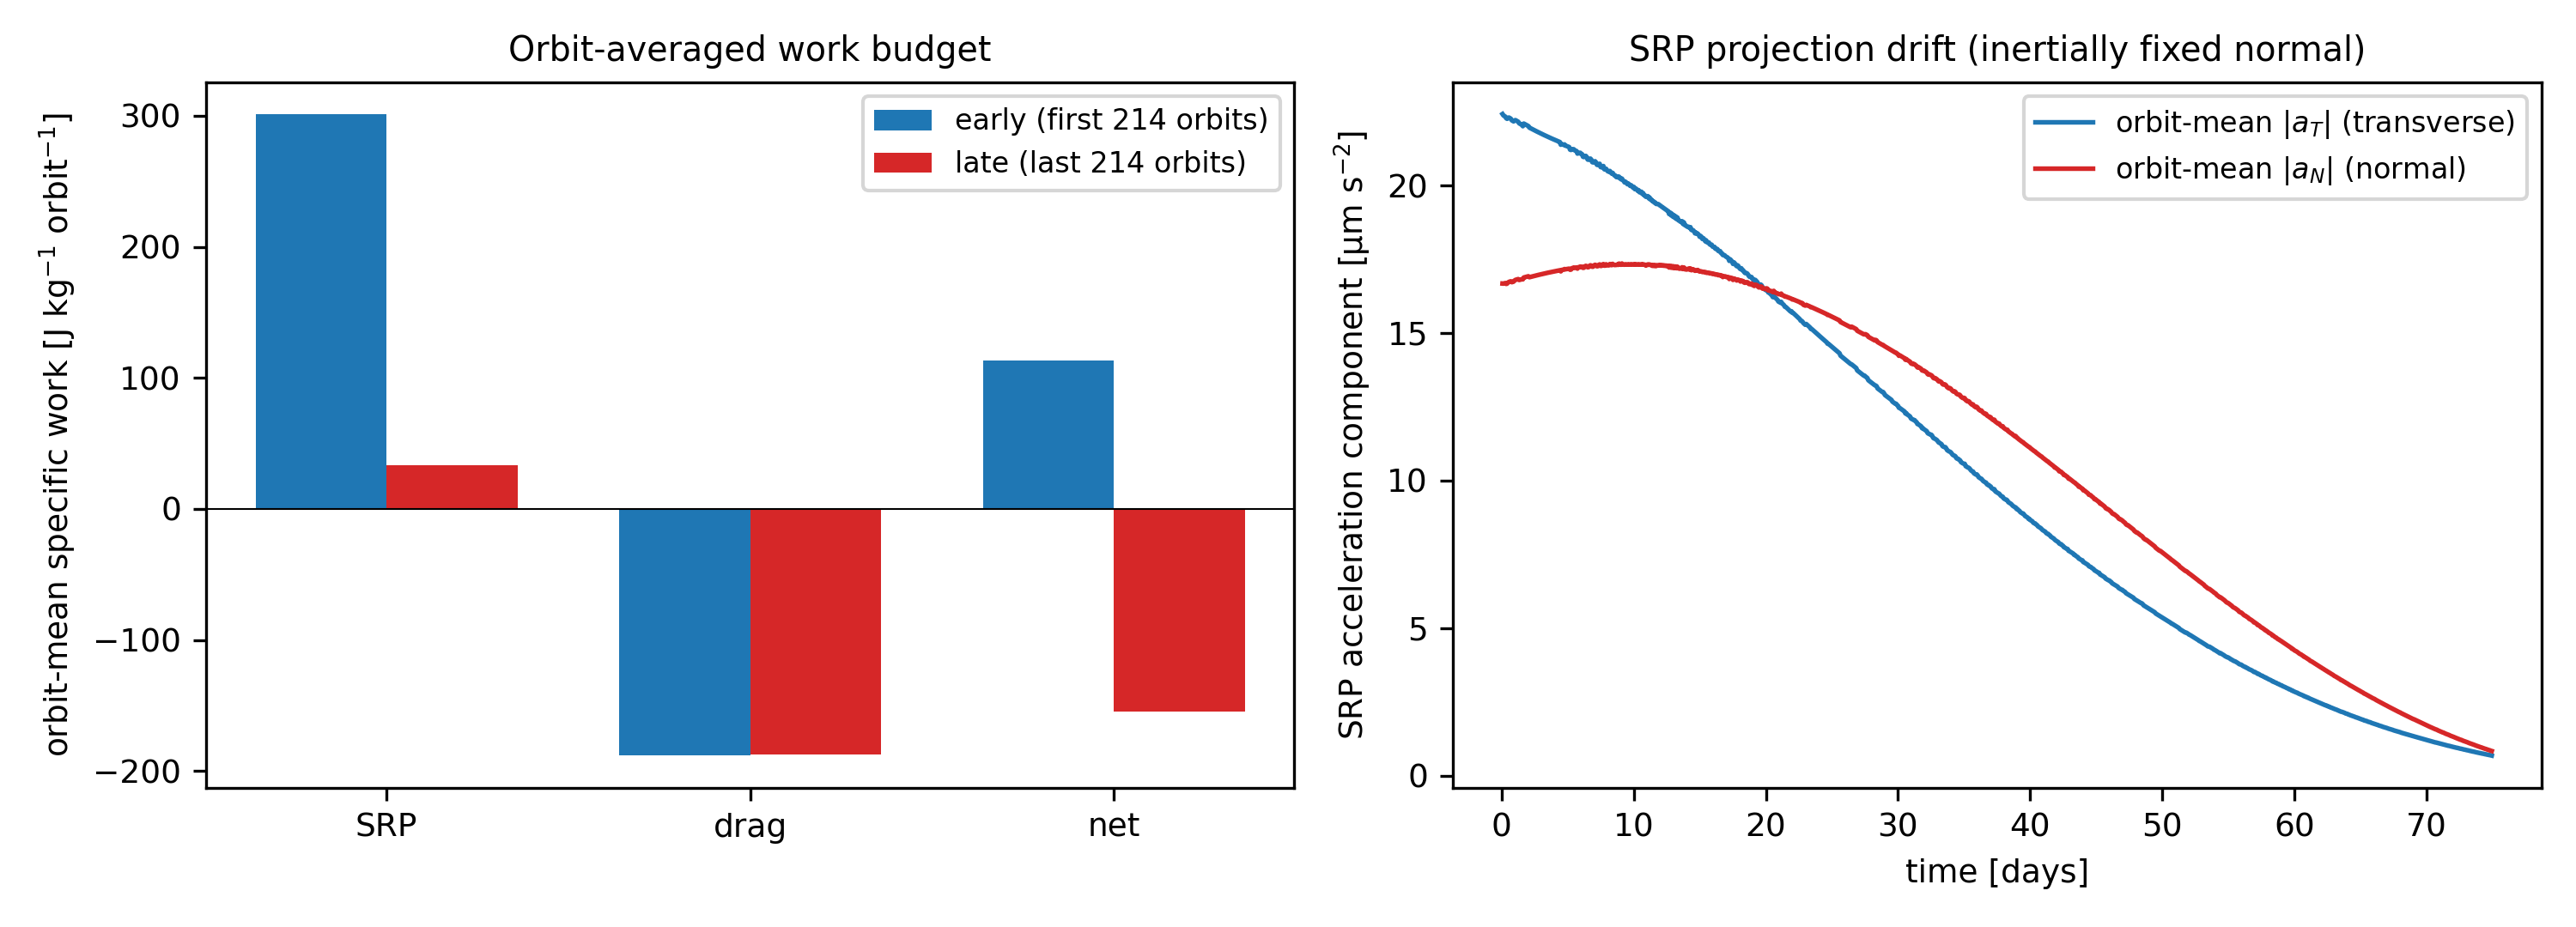
\includegraphics[width=1\linewidth]{Figures/r_earlylate_ftfn.png}
    \setlength{\abovecaptionskip}{0pt}
    \caption{Early-versus-late diagnostics for the representative \(800\,\mathrm{km}\) gain case. Left: orbit-averaged specific SRP, drag and net work (\(\mathrm{J\,kg^{-1}\,orbit^{-1}}\)) in the first and last \(20\%\) windows (\(214\) orbits each); the SRP contribution collapses while the drag penalty is unchanged, so the late-window net balance is negative. Right: orbit-mean transverse \(|a_T|\) and normal \(|a_N|\) components of the SRP acceleration (\(\mu\mathrm{m\,s^{-2}}\)) as functions of time; both fall by more than an order of magnitude as the inertially fixed sail normal drifts away from the Sun line.}
    \label{fig:gaincase_early_late_work_comparison}
\end{figure*}

\vspace{5pt}
\par\noindent This attitude drift is not secondary bookkeeping; it is the dominant late-time effect. Figure~\ref{fig:precession_drift} sketches the geometry. A spin-stabilised sail with its normal fixed in inertial space is well aligned with the Sun at the start of the run, when the pitch of \(+35^\circ\) places the SRP force favourably in the local RT plane during the sunlit arc. Two months later the Sun has moved some \(60^\circ\) along the ecliptic and the orbit plane has precessed with it, while the sail normal has not moved at all. The same inertially fixed attitude therefore sees the Sun at a grazing angle and projects what little force remains less favourably into the local frame. The mechanism established in Section~\ref{sec:existence} requires both the eclipse-induced sign selectivity and a sail that faces the Sun; the first is preserved over \(75\) days, but the second is lost by any attitude that is not actively steered. This is the second breakdown pathway, and in this case the stronger one.

\begin{figure*}[htbp]
    \centering
    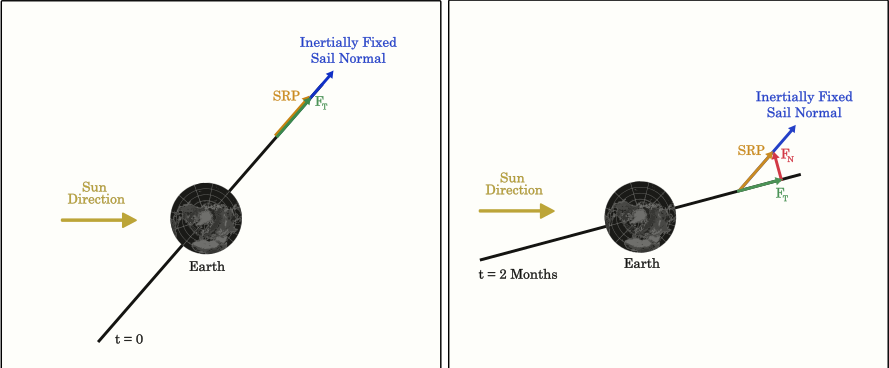
\includegraphics[width=1\linewidth]{Figures/precession.png}
    \caption{Illustration of SRP projection drift for an inertially fixed, spin-stabilised sail in a precessing Sun-synchronous orbit. At \(t=0\) (left), the fixed sail normal is \(35^\circ\) from the Sun line and produces a favourable transverse SRP component \(F_T\). After two months (right), the Sun has moved along the ecliptic and the orbit plane has precessed with it, so the same inertially fixed attitude is illuminated at a grazing angle and projects less favourably into the local frame, with a much reduced \(F_T\) and a relatively larger normal contribution \(F_N\). This geometric drift is the dominant cause of the breakdown of the transient gain regime over the \(75\)-day horizon.}
    \label{fig:precession_drift}
\end{figure*}

\vspace{5pt}
\par\noindent Taken together, the results in this section resolve the apparent tension between early gain and later decay. The mechanism established in Section~\ref{sec:existence} is real, but it is front-loaded and self-limiting. The early positive \(\Delta a\) is achieved mainly through apogee pumping rather than clean whole-orbit lifting; that evolution increases eccentricity and lowers perigee by some \(90\,\mathrm{km}\), which concentrates drag loss, while the inertially fixed sail orientation causes the SRP acceleration to shrink by a factor of about fifty as the Sun--normal angle opens from \(35.0^\circ\) to \(83.4^\circ\). The orbit-averaged balance turns negative on day \(38.1\), at the peak \(\Delta a_{\max,75\mathrm{d}} = +10.86\,\mathrm{km}\); mean \(a\) returns to its initial value on day \(71.0\); and by day \(75\) the cumulative total work is \(-9.9\,\mathrm{kJ\,kg^{-1}}\) with \(\Delta a_{75\mathrm{d}} = -2.69\,\mathrm{km}\). The regime does not fail abruptly; it progressively exhausts the margin that created it, and within the analysed window it exhausts that margin completely. How sensitive this behaviour is to the geometric and physical parameters of the case is the question taken up in Section~\ref{sec:sensitivity}.

\FloatBarrier


\section{Robustness and sensitivity of the gain-anchor case}
\label{sec:sensitivity}
\FloatBarrier
\noindent To assess whether the identified short-horizon gain behaviour is a numerically isolated point or instead occupies a finite bounded neighborhood, a set of local sensitivity sweeps was carried out about the same representative gain-anchor geometry over a fixed \(14\)-day analysis window. In all cases, the response metric is the maximum semi-major-axis increase attained within that window,
\begin{equation}
\Delta a_{\max,14\mathrm{d}} = \max_{t \in [0,14\,\mathrm{d}]} \left(a(t)-a_0\right),
\end{equation}
expressed in kilometres. This is therefore not the final semi-major-axis change at day \(14\), but the largest positive excursion relative to the initial orbit attained at any time within the first \(14\) days.
\vspace{1em}
\noindent The common reference geometry for all three sweeps is defined by \(\Omega = 285.5^\circ\), LTDN \(=12.266176\,\mathrm{hr}\), nominal pitch \(24.8^\circ\), zero roll offset, a \(10\times10\,\mathrm{m}\) sail, and \(A/m = 10\,\mathrm{m^2\,kg^{-1}}\), with the same configuration propagated at both \(700\,\mathrm{km}\) and \(800\,\mathrm{km}\). The corresponding nominal responses are \(\Delta a_{\max,14\mathrm{d}} = 14.958\,\mathrm{km}\) at \(700\,\mathrm{km}\) and \(33.937\,\mathrm{km}\) at \(800\,\mathrm{km}\). The \(800\,\mathrm{km}\) curves should therefore be interpreted as a same-geometry altitude comparison rather than as a separately re-optimised gain anchor.

\vspace{0.5em}
\subsection{\textbf{Static roll sensitivity}}

\par \noindent At the same time, the envelope remains clearly bounded at both altitudes. As the roll magnitude increases beyond roughly \(20^\circ\), the attainable gain decreases steadily, showing that the eclipse-biased work surplus is still alignment-sensitive. The important additional result is that the sensitivity weakens markedly at higher altitude. At \(700\,\mathrm{km}\), offsets of \(\pm45^\circ\) retain only a small fraction of the zero-roll peak, whereas at \(800\,\mathrm{km}\) the same offsets still preserve roughly half of the nominal response. In absolute terms, the \(800\,\mathrm{km}\) case with a \(45^\circ\) roll offset still produces a gain comparable to the zero-roll nominal case at \(700\,\mathrm{km}\). The sweep remains mildly asymmetric about zero, consistent with the present one-sided SRP illumination model, but the dominant result is not the asymmetry itself; it is that the admissible roll envelope broadens substantially once the drag environment is relaxed.
\vspace{1em}

\begin{center}
    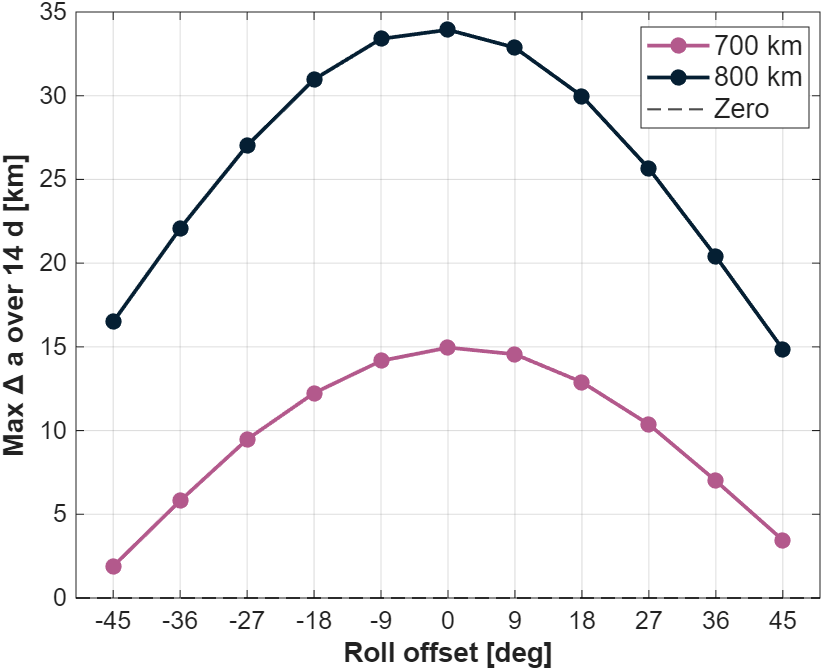
\includegraphics[width=0.92\linewidth]{Figures/fig6_w78.png}
   \captionof{figure}{Sensitivity of the \(14\)-day maximum semi-major-axis increase, \(\Delta a_{\max,14\mathrm{d}}\), to static roll offset about the gain-anchor attitude, shown for the same reference geometry propagated at \(700\,\mathrm{km}\) and \(800\,\mathrm{km}\). The common geometry is \(\Omega = 285.5^\circ\), LTDN \(=12.266176\,\mathrm{hr}\), pitch \(24.8^\circ\), zero roll offset, and \(A/m = 10\,\mathrm{m^2\,kg^{-1}}\). The response peaks at zero roll at both altitudes, but the bounded alignment envelope is substantially broader at \(800\,\mathrm{km}\).}
    \label{fig:roll_sensitivity_gain_anchor}
\end{center}

\vspace{0.5em}
\subsection{\textbf{Sensitivity to atmospheric density level}}

\noindent Figure~\ref{fig:density_sensitivity_gain_anchor} shows the effect of scaling the atmospheric density model by a constant multiplicative factor while holding the gain-anchor geometry fixed at both \(700\,\mathrm{km}\) and \(800\,\mathrm{km}\). At \(700\,\mathrm{km}\), the nominal atmosphere case (\(1\times\)) gives \(\Delta a_{\max,14\mathrm{d}} = 14.96\,\mathrm{km}\), which increases to \(28.59\,\mathrm{km}\) at \(0.5\times\) density and \(34.89\,\mathrm{km}\) at \(0.25\times\). Increasing density, however, suppresses the gain completely at this altitude: at \(2\times\) and \(4\times\) density, \(\Delta a_{\max,14\mathrm{d}} = 0\). At \(800\,\mathrm{km}\), by contrast, the same sweep remains positive throughout the full tested range, with \(33.94\,\mathrm{km}\) at nominal density, \(26.49\,\mathrm{km}\) at \(2\times\), and \(10.25\,\mathrm{km}\) even at \(4\times\) density.
\vspace{1em}
\par \noindent This sweep shows most clearly that drag is the dominant bounding mechanism, but it also shows that the location of the drag-limited boundary depends strongly on altitude. At \(700\,\mathrm{km}\), the short-horizon semi-major-axis increase exists only while the eclipse-biased SRP work surplus exceeds the accumulated drag losses; once the atmosphere is strengthened sufficiently, the drag penalty dominates from the outset and the semi-major axis never rises above its initial value within the \(14\)-day window. At \(800\,\mathrm{km}\), however, the same mechanism remains much more resilient: increased density degrades the gain substantially, but does not eliminate it across the tested range. The most defensible interpretation is therefore not that the regime is uniformly fragile, but that it is strongly altitude-dependent and can lie either near or well away from the drag-limited boundary depending on orbital height.

\begin{center}
     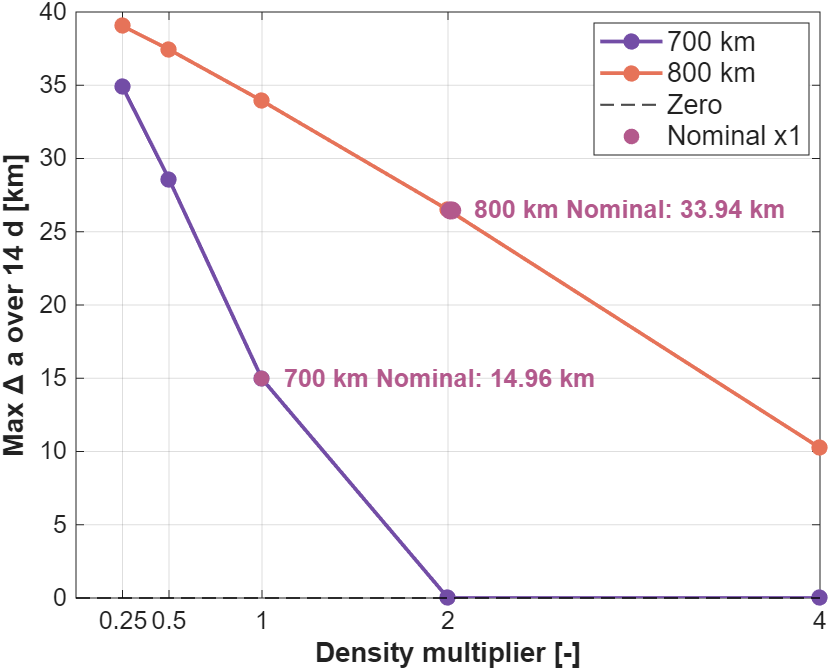
\includegraphics[width=0.92\linewidth]{Figures/fig7_w78.png}
   \captionof{figure}{Sensitivity of the \(14\)-day maximum semi-major-axis increase, \(\Delta a_{\max,14\mathrm{d}}\), to a multiplicative density scaling applied about the same gain-anchor geometry at \(700\,\mathrm{km}\) and \(800\,\mathrm{km}\). Reduced density strengthens the short-horizon gain at both altitudes. Increased density suppresses the \(700\,\mathrm{km}\) response completely by \(2\times\) nominal density, whereas the \(800\,\mathrm{km}\) case remains positive throughout the tested range, showing that the drag-limited boundary shifts substantially with altitude.}
    \label{fig:density_sensitivity_gain_anchor}
\end{center}


\vspace{0.5em}
\subsection{\textbf{Sensitivity to area-to-mass ratio}}

\noindent Figure~\ref{fig:amr_sensitivity_gain_anchor} shows the response to varying area-to-mass ratio while keeping the spacecraft mass fixed at \(10\,\mathrm{kg}\). The square sail side length is varied from \(5\) to \(15\,\mathrm{m}\), corresponding to \(A/m\) values from \(2.5\) to \(22.5\,\mathrm{m^2\,kg^{-1}}\). At \(700\,\mathrm{km}\), the response is non-monotonic. Starting from low \(A/m\), the maximum short-horizon gain rises from \(4.17\,\mathrm{km}\) at \(A/m=2.5\,\mathrm{m^2\,kg^{-1}}\) to the nominal \(14.96\,\mathrm{km}\) at \(A/m=10\,\mathrm{m^2\,kg^{-1}}\), then reaches a broad maximum of \(17.92\,\mathrm{km}\) at \(A/m=14.4\,\mathrm{m^2\,kg^{-1}}\), before declining slightly at larger sail sizes. At \(800\,\mathrm{km}\), by contrast, the response remains monotonic over the full sampled range, rising from \(8.54\,\mathrm{km}\) at \(A/m=2.5\,\mathrm{m^2\,kg^{-1}}\) to \(71.61\,\mathrm{km}\) at \(A/m=22.5\,\mathrm{m^2\,kg^{-1}}\), with no roll-over yet visible.
\vspace{1em}
\par \noindent The altitude split again changes the interpretation. At \(700\,\mathrm{km}\), the non-monotonicity shows that increasing sail size does not produce indefinite improvement: larger \(A/m\) strengthens SRP, but it also strengthens drag and modifies the coupled orbital response over the \(14\)-day window, producing a finite optimum and then a shallow plateau. At \(800\,\mathrm{km}\), however, the same drag-induced roll-over is pushed beyond the sampled range, so increasing \(A/m\) continues to improve the short-horizon gain throughout the tested envelope. The shared conclusion is that stronger SRP authority is beneficial, but the accessible benefit depends on how strongly drag competes over the observation window. Compared with the density sweep, the \(A/m\) response remains broad at both altitudes, but only the lower-altitude case shows a clear local optimum within the sampled range.

\begin{center}
    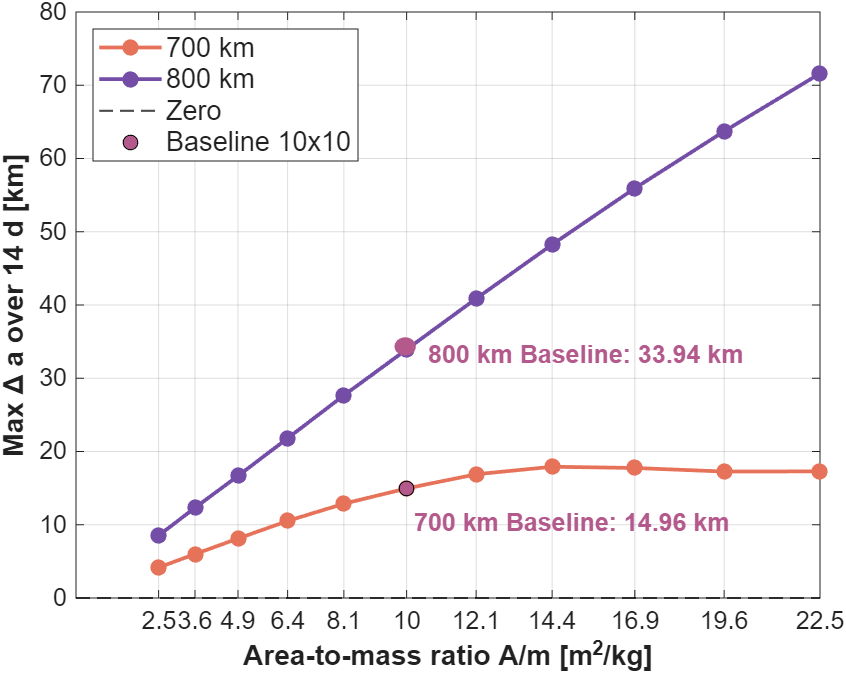
\includegraphics[width=1\linewidth]{Figures/fig8_w78.png}
    \captionof{figure}{Sensitivity of the \(14\)-day maximum semi-major-axis increase, \(\Delta a_{\max,14\mathrm{d}}\), to sail area-to-mass ratio for the gain-anchor case, with spacecraft mass held fixed at \(10\,\mathrm{kg}\), shown for the same reference geometry at \(700\,\mathrm{km}\) and \(800\,\mathrm{km}\). The \(700\,\mathrm{km}\) response is non-monotonic, with a broad optimum near \(A/m = 14.4\,\mathrm{m^2\,kg^{-1}}\), whereas the \(800\,\mathrm{km}\) response continues to increase across the full sampled range.}
    \label{fig:amr_sensitivity_gain_anchor}
\end{center}

\vspace{0.5em}
\subsection{\textbf{Interpretation of the sensitivity envelope}}

\noindent Taken together, the three sweeps support a restrained but more nuanced conclusion. The transient gain behaviour is not a numerically singular point: it persists over a finite neighborhood in roll and over a broad range of positive \(A/m\), and this admissible neighborhood expands significantly between \(700\,\mathrm{km}\) and \(800\,\mathrm{km}\). At the same time, the mechanism is still not a generally robust passive orbit-raising mode. Its existence remains contingent on favourable Sun-orbit-attitude phasing and on a drag environment weak enough for the eclipse-biased SRP work surplus to remain positive over the observation window.
\vspace{1em}
\par \noindent The most defensible statement is therefore that the gain occupies a bounded local envelope whose size depends materially on altitude. Roll sensitivity demonstrates finite but limited alignment tolerance at \(700\,\mathrm{km}\), but a substantially wider tolerance band at \(800\,\mathrm{km}\). Density sensitivity shows that drag remains the dominant bounding mechanism, while also showing that the regime can lie either close to or well away from the drag-dominated breakdown threshold depending on orbital height. Area-to-mass sensitivity shows that stronger SRP authority improves the short-horizon gain broadly, but that the onset of diminishing returns is itself altitude-dependent and is shifted to larger \(A/m\) at higher altitude. These results are consistent with the broader thesis of the paper: the mechanism is real and physically interpretable, but it is geometry-bounded, alignment-sensitive, and ultimately limited by the coupled drag and orbital-distortion effects that later drive the long-horizon transition from transient gain to decay.

\FloatBarrier

\section{Independent numerical validation: an open-source propagator cross-checked against STK Astrogator and Orekit}
\label{sec:validation}
\FloatBarrier
\noindent The results of Sections~\ref{sec:existence}--\ref{sec:sensitivity} were produced by a single open-source propagator written for this class of passive-sail SRP--drag problem. Because the gain regime is narrow and rests on a delicate balance between eclipse-gated SRP work and atmospheric drag, its credibility depends on two things being demonstrated independently: first, that the gain region \emph{exists} and is not an artefact of one numerical implementation; and second, that the propagator used to map it is itself trustworthy. This section addresses both by cross-validating that propagator, component by component, against two independent references: Ansys Systems Tool Kit (STK) with the Astrogator module \citep{ansysSTK2024,shortRevisitingTrajectory2019}, a widely used industry-standard flight-dynamics environment, for the conservative dynamics, the application of drag and, after two configuration corrections described below, the SRP response; and the Orekit library \citep{orekit} for the force models, the gain regime itself, and the sensitivity of the results to the atmosphere model and the solar ephemeris.

\vspace{5pt}
\par\noindent The motivation is practical as well as methodological. Solar-sail and drag-sail concepts are increasingly demonstrated in low Earth orbit on low-cost CubeSat and small-satellite platforms --- NanoSail-D \citep{johnsonNanoSailD2011}, CubeSail \citep{lappasCubeSail2011}, InflateSail \citep{underwoodInflateSail2019}, and CanX-7 \citep{boninCanX72013} --- precisely because LEO offers a cost-effective, rapidly accessible test environment for maturing sail technology before committing to expensive deep-space missions \citep{selvaCubeSatSurvey2012,woellertCubeSatCost2011}. Reliable pre-flight prediction of the coupled SRP--drag dynamics for such demonstrators requires propagation tools whose force models have been verified against a recognised reference. Open-source propagators (GMAT \citep{hughesGMATVV2014}, Orekit \citep{orekit}, poliastro \citep{canoPoliastro2022}, Basilisk \citep{kenneallyBasilisk2020}, Tudat \citep{dirkxTudatpy2022}) make such studies reproducible and inspectable, but they must be validated; cross-checking an open-source propagator against STK/HPOP is an established verification practice \citep{refaatPropagatorValidation2018,hughesGMATVV2014}.

\subsection{Open-source propagator}
\label{sec:val_propagator}
\noindent The propagator integrates the equations of motion of Section~\ref{sec:model} directly in Cartesian ECI coordinates with a fixed-step fourth-order Runge--Kutta scheme at a production step of \(10\,\mathrm{s}\) (chosen in Section~\ref{sec:val_convergence}). The force model comprises: (i) central gravity with the \(J_2\) zonal term; (ii) atmospheric drag with the frontal area \(A\lvert\cos\theta\rvert\) projected onto the instantaneous inertial velocity, no atmospheric co-rotation, and the U.S.\ Standard Atmosphere 1976 density \citep{USSA1976} evaluated at the geocentric altitude and interpolated exponentially (log-linearly) between the tabulated values (Section~\ref{sec:model}); and (iii) solar radiation pressure from a single one-sided flat plate with absorptivity \(\alpha_a = 0.3\), specular reflectivity \(\rho_s = 0.7\) and diffuse reflectivity \(\rho_d = 0\), so that the normal-incidence coefficient is \(C_r = 1.7\) (Table~\ref{tab:baseline_params}), with the solar flux scaled by \((1\,\mathrm{AU}/d_{\odot})^2\) using the analytic Sun of Section~\ref{sec:model}. A binary cylindrical umbra gates the SRP. The sail normal is constructed once, at epoch, from the LTAN, inclination and pitch angle and then frozen in inertial space, consistent with the passively spin-stabilised assumption. Mean (secular) elements are recovered by stroboscopic sampling of the osculating semi-major axis at ascending-node crossings, the first sample falling one nodal period after epoch; this removes the \(\pm 9\,\mathrm{km}\) \(J_2\) short-period signature that would otherwise mask the few-kilometre secular signal of interest. A run stops when the perigee altitude falls below \(120\,\mathrm{km}\), which is reported as re-entry.

\vspace{5pt}
\par\noindent The SRP plate uses the physically consistent specular/diffuse/absorptive decomposition of the flat-plate force \citep{mcmahonSchereesSRP2010,montenbruckGill2000}, which places the specular component along the plate normal with a \(\cos^2\alpha\) dependence, exactly the form of Eq.~\eqref{eq:srp_vector}; its agreement with the \(C_r\cos^2\alpha\) law is checked against Orekit's independent plate implementation in Section~\ref{sec:val_orekit}. We emphasise that the along-normal (specular) direction is essential: an SRP force of the same magnitude directed along the Sun line performs zero net orbit-averaged work in this geometry, because the positive and negative arcs cancel, so only the normal-directed plate reproduces the eclipse-gated pumping mechanism. Section~\ref{sec:existence} quantifies this at the gain anchor: \(\Delta a(14\,\mathrm{d}) = +5.95\,\mathrm{km}\) with the plate, \(-9.89\,\mathrm{km}\) without SRP, and \(-10.50\,\mathrm{km}\) with the Sun-line variant of the force.

\subsection{Step-size convergence}
\label{sec:val_convergence}
\noindent The umbra makes the SRP force discontinuous in time, and a fixed-step integrator that straddles the shadow boundary commits an error of first order in the step at every eclipse entry and exit. Figure~\ref{fig:convergence} shows the consequence for the \(14\)-day node-sampled \(\Delta a(14\,\mathrm{d})\) at the \(800\,\mathrm{km}\) gain anchor and at the former \(700\,\mathrm{km}\) anchor for three configurations: the full model, the full model with the umbra disabled, and drag only. At \(800\,\mathrm{km}\) the full model gives \(-1.9898\), \(+5.6508\), \(+5.9329\), \(+5.9521\), \(+5.9508\), \(+5.9546\), \(+5.9538\) and \(+5.9556\,\mathrm{km}\) at \(\Delta t = 120\), \(60\), \(30\), \(15\), \(10\), \(7.5\), \(5\) and \(2.5\,\mathrm{s}\), against \(+5.9401\,\mathrm{km}\) for an adaptive Dormand--Prince 8(5,3) (DP853) reference in Orekit with eclipse event detection, which places the integration steps exactly on the shadow boundaries. The two smooth configurations converge by \(30\,\mathrm{s}\): the umbra-disabled model gives \(-10.5934\,\mathrm{km}\) at \(30\,\mathrm{s}\) and \(-10.5873\,\mathrm{km}\) at \(10\,\mathrm{s}\) against the DP853 value of \(-10.5864\,\mathrm{km}\), and drag only gives \(-9.9091\) and \(-9.8938\,\mathrm{km}\) against \(-9.8989\,\mathrm{km}\). Running the same RK4 ladder inside Orekit confirms that the behaviour belongs to the problem, not to the implementation: a least-squares fit gives an observed convergence order of \(0.94\) for the eclipse-gated model, against the nominal fourth order, while the smooth configurations are already converged to within about \(0.01\,\mathrm{km}\) at \(30\,\mathrm{s}\) so that no meaningful order can be fitted. The coarse-step error is also non-asymptotic: in the Orekit ladder the \(60\,\mathrm{s}\) result (\(+7.229\,\mathrm{km}\)) overshoots the reference by more than the \(120\,\mathrm{s}\) result (\(+6.068\,\mathrm{km}\)), and in the present propagator the \(120\,\mathrm{s}\) step reverses the sign of the result while \(60\,\mathrm{s}\) undershoots by \(0.3\,\mathrm{km}\). Accuracy therefore cannot be inferred from the step size alone for this problem; it must be established against an event-detecting reference. The production step of \(10\,\mathrm{s}\) reproduces the DP853 reference to \(+0.18\%\) (\(+5.9508\) against \(+5.9401\,\mathrm{km}\)); at \(700\,\mathrm{km}\) the full model gives \(-21.0735\,\mathrm{km}\) at \(10\,\mathrm{s}\) against \(-21.0640\,\mathrm{km}\) at \(2.5\,\mathrm{s}\).

\begin{figure*}[htbp]
    \centering
    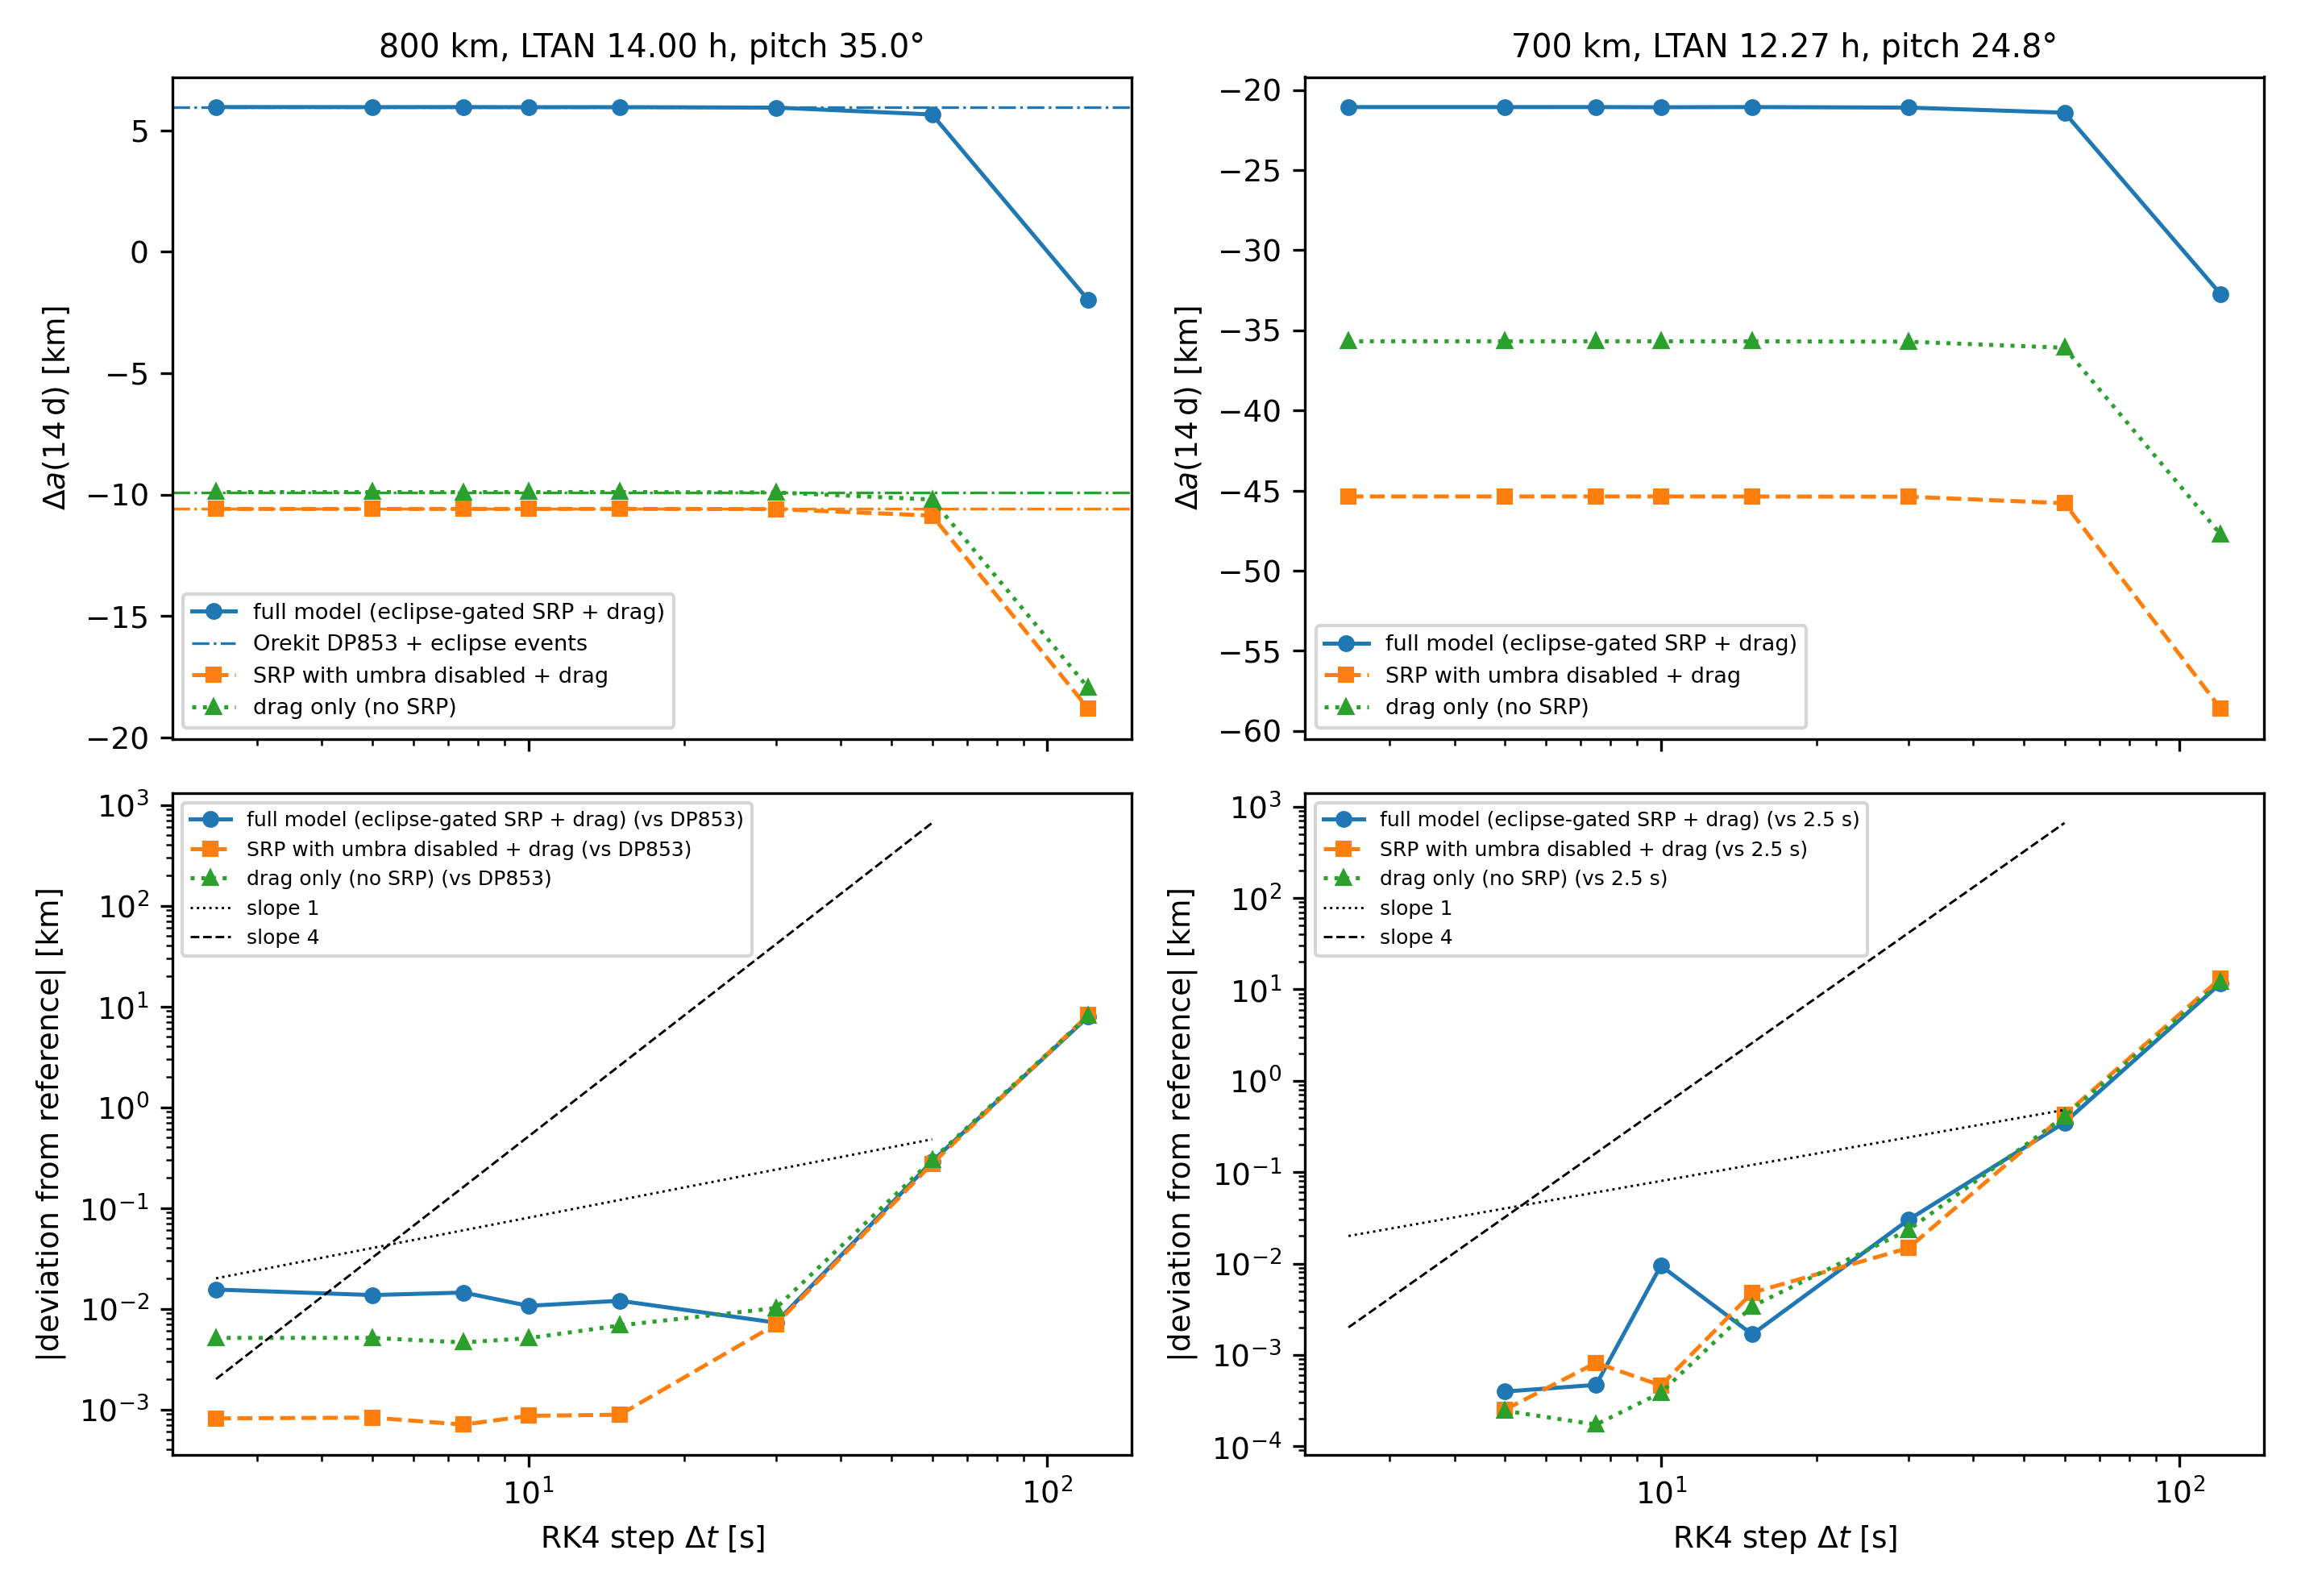
\includegraphics[width=1\linewidth]{Figures/r_convergence.png}
    \setlength{\abovecaptionskip}{0pt}
    \caption{Step-size convergence of the node-sampled \(\Delta a(14\,\mathrm{d})\) for fixed-step RK4 at \(\Delta t = 120\) to \(2.5\,\mathrm{s}\), at the \(800\,\mathrm{km}\) gain anchor (left; LTAN \(14.0\,\mathrm{h}\), pitch \(+35^\circ\)) and the former \(700\,\mathrm{km}\) anchor (right; LTAN \(12.266\,\mathrm{h}\), pitch \(+24.8^\circ\)) for the full model, the full model with the umbra disabled, and drag only. Dash-dot lines are the Orekit DP853 references with eclipse event detection at \(800\,\mathrm{km}\): \(+5.9401\), \(-10.5864\) and \(-9.8989\,\mathrm{km}\). Lower row: absolute deviation from the reference (the DP853 value at \(800\,\mathrm{km}\); the \(2.5\,\mathrm{s}\) RK4 result at \(700\,\mathrm{km}\), where no Orekit reference was run) with first- and fourth-order slope guides. The smooth configurations converge by \(30\,\mathrm{s}\); the eclipse-gated model converges only slowly (observed order about one in the Orekit ladder) and settles within \(0.02\,\mathrm{km}\) of the reference below \(15\,\mathrm{s}\); the production step of \(10\,\mathrm{s}\) reproduces the reference to \(0.18\%\).}
    \label{fig:convergence}
\end{figure*}

\subsection{STK Astrogator configuration}
\label{sec:val_stkconfig}
\noindent The STK reference cases were built with Ansys STK Engine 13.0.1 (Premium; installer \texttt{Ansys\_STK\_Premium\_\allowbreak ODTK\_v13.0.1}), driven headlessly through the \texttt{agi.stk13} Object Model from CPython 3.12 on Windows 11, so that the sweeps could be executed without the graphical interface. Each satellite uses the Astrogator propagator: a Mission Control Sequence with an Initial State segment (Keplerian elements in the Earth ICRF frame, epoch 1 Jan 2026 12:00 UTC) and a Propagate segment terminated on a Duration stopping condition. A numerical propagator cloned from ``Earth Point Mass'' carries three propagator functions configured to match the paper's model: ``Gravitational Force'' truncated to degree~2, order~0 (\(J_2\) only, tides off); ``US Standard Atmosphere'' (1976) with the spherical area model for the attitude-independent validation and the N-plate model otherwise; and ``NPlate SRP'' with the cylindrical shadow and a mean flux of \(1367.2\,\mathrm{W\,m^{-2}}\), equal to \(P_{1\,\mathrm{AU}}c\) of the open-source plate. The plate files define one body \(+Z\) SRP plate (area \(100\,\mathrm{m^2}\), specular reflectivity \(0.70\), diffuse \(0.00\)) and two opposed \(\pm Z\) drag plates (\(C_D = 2.2\)), so that the projected drag area follows \(A\lvert\cos\theta\rvert\). The inertially fixed attitude is imposed with the \texttt{eProfileFixedInAxes} profile referenced to Earth ICRF and the quaternion mapping body \(+Z\) onto the sail normal. Osculating elements are read from the Classical Elements data provider every \(60\,\mathrm{s}\); for both tools the mean semi-major axis of this comparison is the centred one-period average of the osculating value, and the quoted change is taken between \(t = T/2\) and \(t = T/2 + 14\,\mathrm{d}\), so that it spans exactly \(14\) days. (The open-source values in Table~\ref{tab:stk_validation} therefore differ slightly from the node-sampled values used elsewhere in the paper, e.g.\ \(+5.85\) against \(+5.95\,\mathrm{km}\) at the gain anchor.)

\vspace{5pt}
\par\noindent A script-based force-plugin route was attempted first and then abandoned. The Python force-model plugins of STK~13 require a registered COM server implementing the drag and SRP plugin interfaces, and registration failed on this installation. The attempt is documented in the repository, and the built-in N-plate models were used instead. Faceted and N-plate SRP models of this kind are the standard higher-fidelity representation in the flight-dynamics literature \citep{ziebartGeneralizedSRP2004,ziebartDarePixelArray2001,rodriguezsolanoBoxWing2012,vielbergRadiationPressure2020}, but they are configured through several layers of objects whose effective values are not all visible through the properties one sets; the comparison below therefore reads STK's \emph{effective} inputs back along the trajectory through the ``Astrogator Values'' data providers (applied density, drag area, SRP area, mass) rather than trusting the configured ones.

\vspace{5pt}
\par\noindent That read-back exposed two configuration errors in the STK build of the originally submitted version, which must be stated plainly because they account for its two principal findings. (i) The Initial State segment's fuel tank carried its default \(50\,\mathrm{kg}\) of fuel, which Astrogator adds to the \(10\,\mathrm{kg}\) dry mass when evaluating drag and SRP. The submitted STK runs therefore propagated a \(60\,\mathrm{kg}\) vehicle, \(A/m = 1.67\) instead of \(10\,\mathrm{m^2\,kg^{-1}}\), while every read-back property (dry mass, drag area, \(C_D\), density) looked correct because the fuel mass is stored elsewhere. This is the whole of the ``order-of-magnitude'' drag discrepancy of the submitted version (\(-7.4\,\mathrm{km}\) for STK against \(-84\,\mathrm{km}\) for the open-source propagator at \(700\,\mathrm{km}\)): with the tank zeroed, the \(14\)-day spherical-drag decay changes from \(-7.48\) to \(-60.30\,\mathrm{km}\) at \(700\,\mathrm{km}\) and from \(-2.77\) to \(-17.68\,\mathrm{km}\) at \(800\,\mathrm{km}\) (Table~\ref{tab:stk_validation}). (ii) The Object Model's \texttt{AssignQuaternion} method (interface \texttt{IAgOrientationQuaternion}) takes \((q_x, q_y, q_z, q_s)\) with the scalar component last, and had been called scalar-first. The resulting attitude mis-oriented the plate: STK's effective Sun-facing area at epoch read \(16.43\,\mathrm{m^2}\) where \(A\cos\alpha = 82.90\,\mathrm{m^2}\) was expected (probe at pitch \(34^\circ\)), and the \(3\)-day \(J_2\)+SRP response was \(+0.21\,\mathrm{km}\) against \(+3.28\,\mathrm{km}\) for the open-source propagator. This, not a limitation of the N-plate model, was the origin of the ``N-plate model does not use the attitude'' finding of the submitted version. With the Object-Model component order the effective area reads \(82.96\,\mathrm{m^2}\) and the \(3\)-day response \(+3.29\,\mathrm{km}\); at the \(35^\circ\) gain anchor the effective area is \(81.97\,\mathrm{m^2}\) (\(A\cos 35^\circ = 81.92\,\mathrm{m^2}\)), and at the former \(24.8^\circ\) anchor \(90.77\,\mathrm{m^2}\) (\(90.78\,\mathrm{m^2}\)). STK's SRP response then matches the open-source propagator, as the next subsection shows.

\subsection{Cross-validation against STK}
\label{sec:val_stk}
\noindent Figure~\ref{fig:stk_validation} and Table~\ref{tab:stk_validation} compare the two tools configuration by configuration. For the conservative dynamics (two-body plus \(J_2\), drag and SRP disabled) the centred-mean semi-major axes are identical to the metre level: the maximum absolute difference over the \(14\)-day window is \(0.25\,\mathrm{m}\) at \(700\,\mathrm{km}\) and \(0.16\,\mathrm{m}\) at \(800\,\mathrm{km}\), confirming the gravitational model, the coordinate handling and the mean-element extraction of the open-source propagator.

\vspace{5pt}
\par\noindent For \(J_2\) plus spherical drag, with the fuel tank corrected, STK gives \(-60.295\,\mathrm{km}\) against \(-70.564\,\mathrm{km}\) for the open-source propagator at \(700\,\mathrm{km}\) (ratio \(0.854\)) and \(-17.678\) against \(-18.547\,\mathrm{km}\) at \(800\,\mathrm{km}\) (ratio \(0.953\)); with the N-plate drag model at the gain-anchor attitude the corresponding values are \(-27.972\) against \(-31.524\,\mathrm{km}\) (ratio \(0.887\)) at \(700\,\mathrm{km}\) and \(-9.446\) against \(-10.015\,\mathrm{km}\) (ratio \(0.943\)) at \(800\,\mathrm{km}\). The as-submitted default-tank values of \(-7.482\) and \(-2.770\,\mathrm{km}\) are plotted dotted in panel (b) and listed in the table for the record. The residual \(5\)--\(15\%\) is a difference of convention, not of force magnitude. Astrogator applies a co-rotating atmosphere and evaluates the density at the geodetic altitude, whereas the paper's model uses the inertial velocity and the geocentric altitude. Orekit, switching these one at a time with everything else fixed (Section~\ref{sec:val_drag}), gives factors of \(\times1.034\) (co-rotation) and \(\times0.816\) (geodetic altitude) at \(700\,\mathrm{km}\), \(\times1.024\) and \(\times0.901\) at \(800\,\mathrm{km}\), and \(\times0.842\) and \(\times0.922\) combined, which accounts for the STK/open-source ratios to within about \(1.5\%\) at \(700\,\mathrm{km}\) and \(3\%\) at \(800\,\mathrm{km}\). The density STK actually applied, read back along the trajectory, averages \(0.887\) (range \(0.757\)--\(1.032\), over \(632\)--\(699\,\mathrm{km}\)) and \(0.937\) (range \(0.839\)--\(1.040\), over \(774\)--\(799\,\mathrm{km}\)) of the open-source value at the same geocentric altitude, consistent with the geodetic-altitude evaluation. For the extreme area-to-mass ratio of a sail (\(A/m = 10\,\mathrm{m^2\,kg^{-1}}\)) atmospheric drag is the dominant and least portable element of the force model \citep{anselmoHAMR2010}, and these conventions must be stated for any LEO sail prediction to be reproducible; they are now stated in Section~\ref{sec:model}.

\vspace{5pt}
\par\noindent With the quaternion corrected, STK's N-plate SRP response at the gain anchor agrees with the open-source plate: \(+15.554\) against \(+15.565\,\mathrm{km}\) over \(14\) days with eclipse on (maximum difference \(0.014\,\mathrm{km}\), about \(0.1\%\)), and \(+0.004\) against \(+0.006\,\mathrm{km}\) with the umbra removed, so both tools reproduce the cancellation of the orbit-averaged SRP work under continuous illumination that Section~\ref{sec:physics} predicts. For the full model at the gain anchor STK gives \(+6.441\,\mathrm{km}\) with eclipse on and \(-10.134\,\mathrm{km}\) with it off, against \(+5.846\) and \(-10.927\,\mathrm{km}\) for the open-source propagator: the eclipse-driven sign reversal of Section~\ref{sec:existence} is reproduced, and STK's slightly larger gain follows directly from its \(5\%\) weaker drag. Over \(75\) days STK reproduces the transient signature of Section~\ref{sec:breakdown}: its mean semi-major axis peaks at \(+12.92\,\mathrm{km}\) on day \(41.9\) and ends at \(+2.56\,\mathrm{km}\), against a peak of \(+10.60\,\mathrm{km}\) on day \(38.0\) and \(-2.70\,\mathrm{km}\) at day \(75\) for the open-source propagator under the centred-mean definition (\(+10.86\,\mathrm{km}\) on day \(38.1\) and \(-2.69\,\mathrm{km}\) node-sampled, Table~\ref{tab:cases}); the end-point difference of \(5.3\,\mathrm{km}\) is the drag-convention difference accumulated over \(1069\) orbits of decay. At the former \(700\,\mathrm{km}\) anchor the full model decays in both tools, \(-17.357\,\mathrm{km}\) in STK against \(-21.548\,\mathrm{km}\).

\begin{figure*}[htbp]
    \centering
    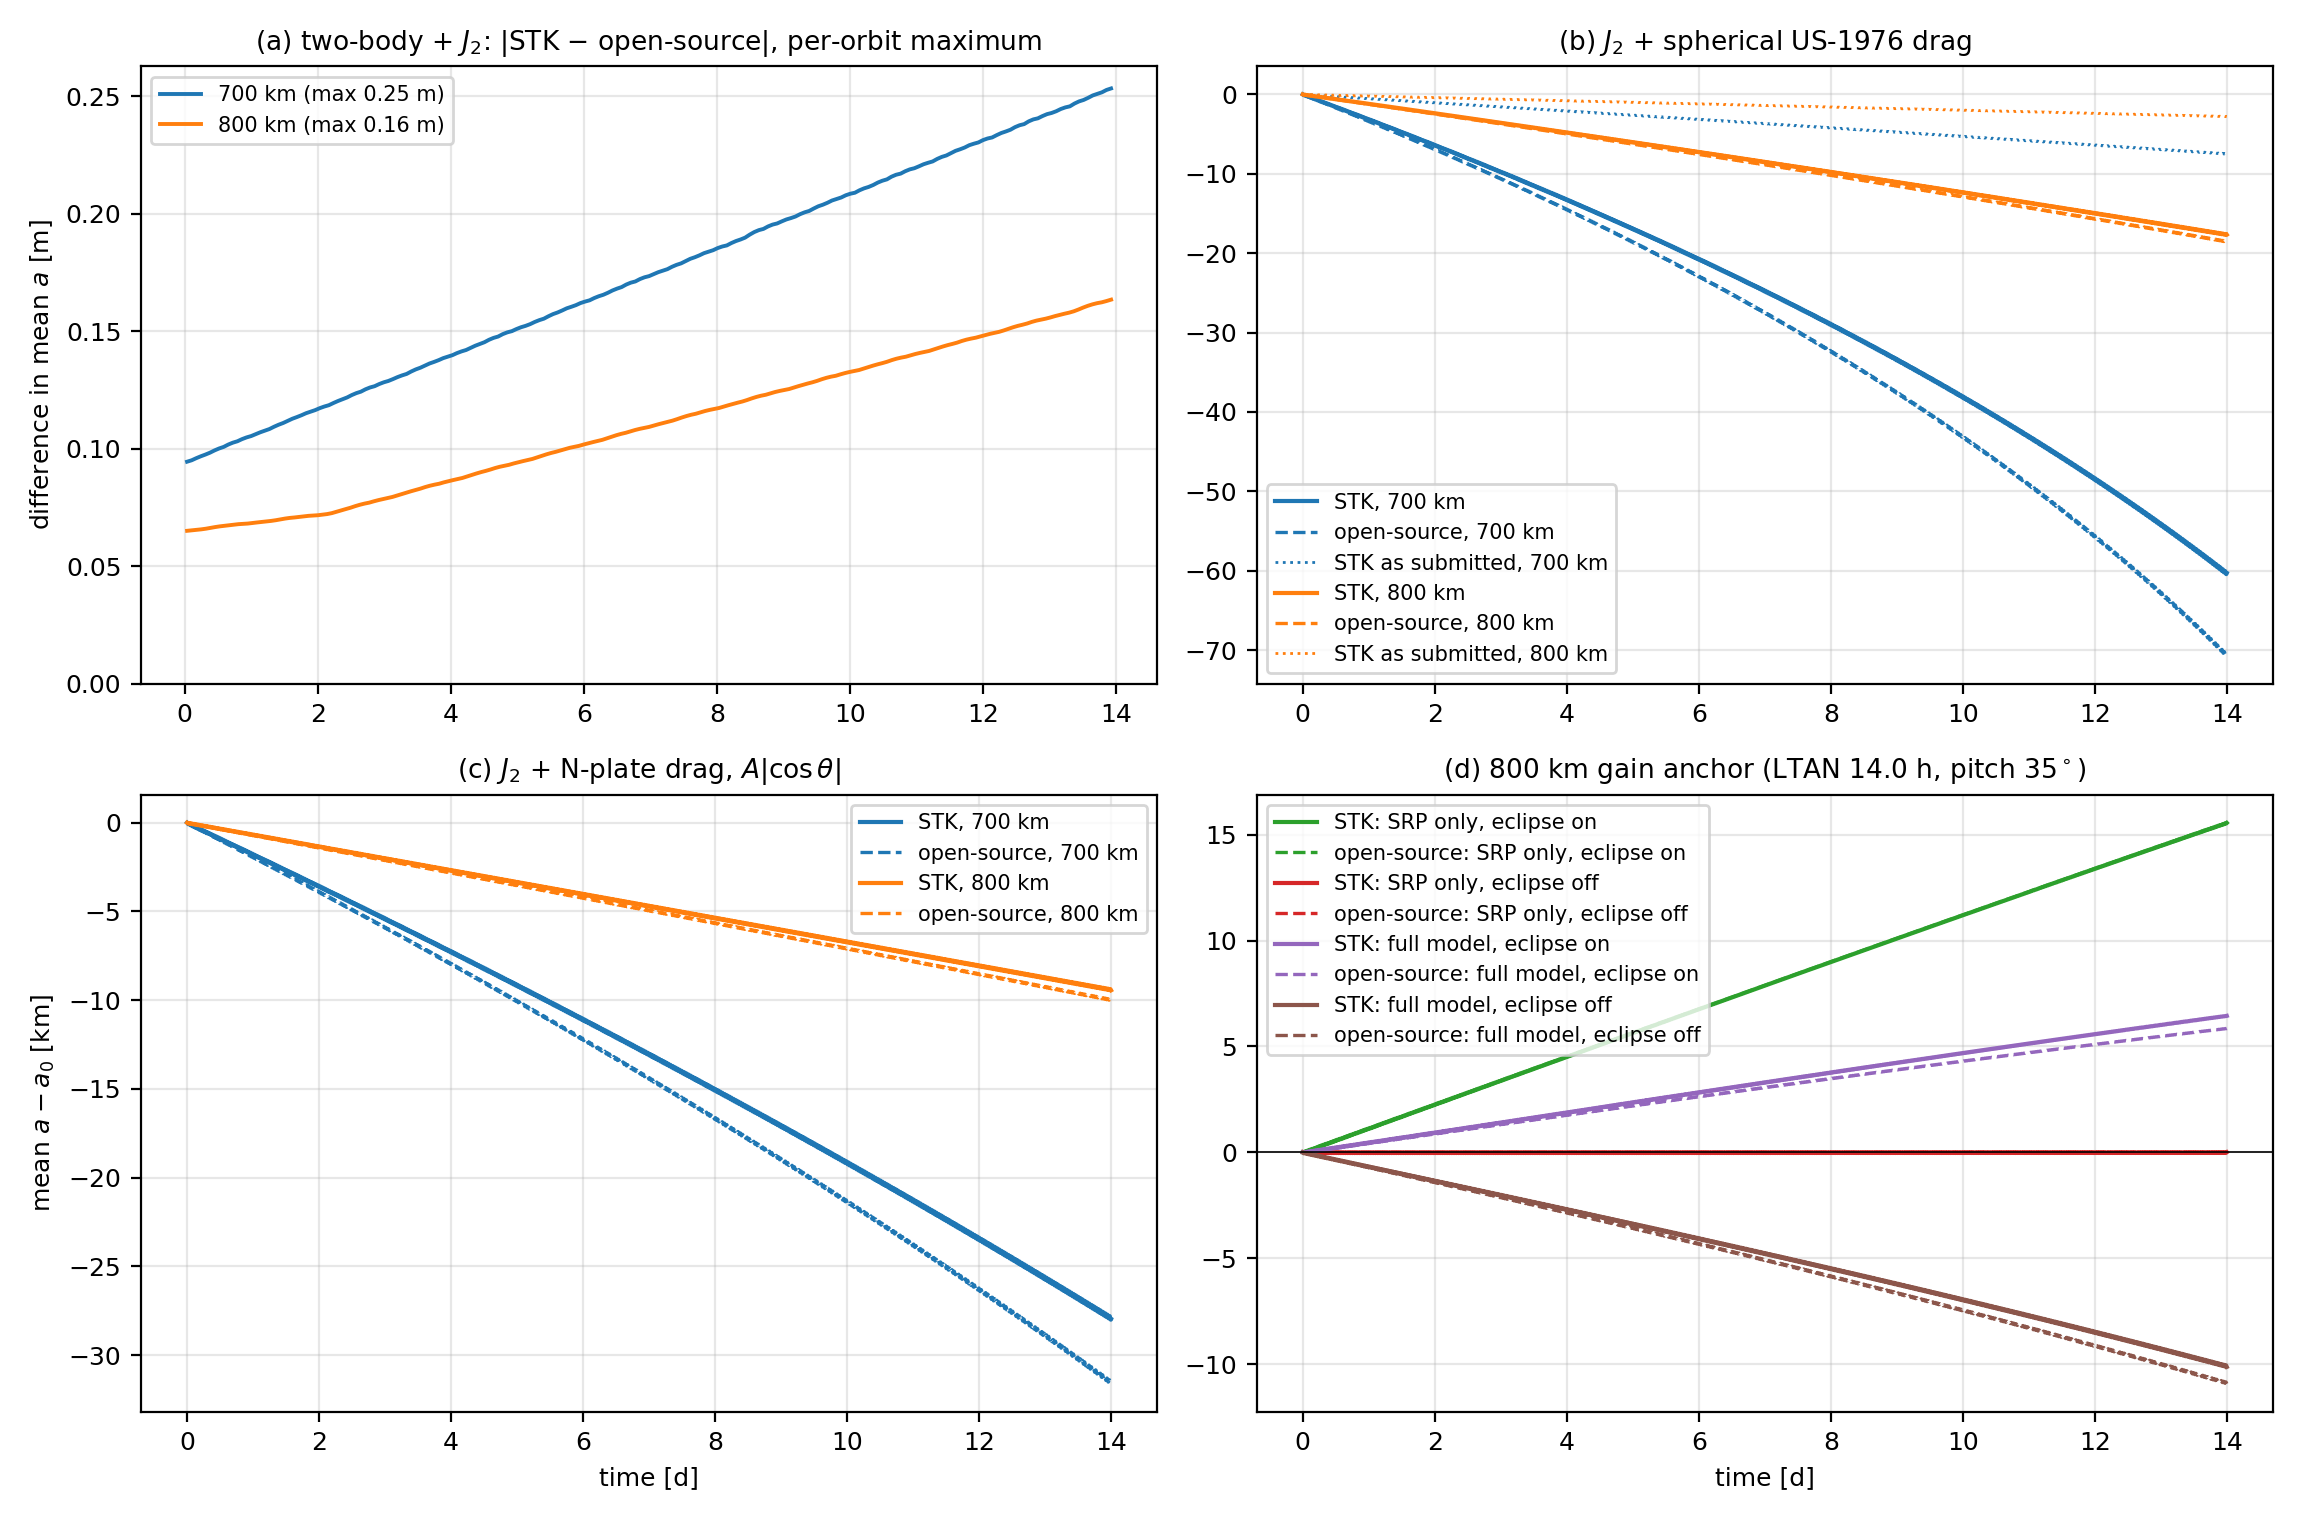
\includegraphics[width=1\linewidth]{Figures/r_stk_validation.png}
    \setlength{\abovecaptionskip}{0pt}
    \caption{Cross-validation of the open-source propagator against STK Astrogator (STK Engine 13.0.1), centred one-period mean semi-major axis over \(14\) days. (a) Two-body plus \(J_2\) at \(700\) and \(800\,\mathrm{km}\): per-orbit maximum of the absolute difference between the two tools, which stays below \(0.25\,\mathrm{m}\) over \(14\) days. (b) \(J_2\) plus spherical U.S.\ Standard Atmosphere 1976 drag with the fuel tank corrected (solid) and the as-submitted default-tank curves (dotted). (c) \(J_2\) plus N-plate drag at the gain-anchor attitude. (d) SRP only and the full model at the \(800\,\mathrm{km}\) gain anchor with eclipse on and off; the sign reversal under eclipse is reproduced by both tools.}
    \label{fig:stk_validation}
\end{figure*}

\begin{table*}[htbp]
\centering
\caption{Cross-validation against STK Astrogator: change in the centred one-period mean semi-major axis over \(14\) days (\(75\) days for the last two rows), STK against the open-source propagator (OS), the ratio STK/OS, and the maximum absolute difference \(\max\lvert\Delta\rvert\) between the two over the window; all changes in km. Gain anchor LTAN \(14.0\,\mathrm{h}\), pitch \(+35^\circ\); the former-anchor row uses LTAN \(12.266\,\mathrm{h}\), pitch \(+24.8^\circ\). The ``default tank'' rows are the build of the original submission (\(60\,\mathrm{kg}\) vehicle), shown for the record.}
\label{tab:stk_validation}
\vspace{0.5em}
\footnotesize
\setlength{\tabcolsep}{3pt}
\begin{tabular}{l c r r r r}
\toprule
Configuration & Alt.\ [km] & STK & OS & STK/OS & \(\max\lvert\Delta\rvert\) \\
\midrule
Two-body + \(J_2\) & 700 & \(-0.055\) & \(-0.055\) & \(0.999\) & \(0.0003\) \\
Two-body + \(J_2\) & 800 & \(-0.000\) & \(-0.000\) & --- & \(0.0002\) \\
\(J_2\) + spherical drag, default tank & 700 & \(-7.482\) & \(-70.564\) & \(0.106\) & \(63.196\) \\
\(J_2\) + spherical drag, default tank & 800 & \(-2.770\) & \(-18.547\) & \(0.149\) & \(15.817\) \\
\(J_2\) + spherical drag, corrected & 700 & \(-60.295\) & \(-70.564\) & \(0.854\) & \(10.535\) \\
\(J_2\) + spherical drag, corrected & 800 & \(-17.678\) & \(-18.547\) & \(0.953\) & \(0.885\) \\
\(J_2\) + N-plate drag & 700 & \(-27.972\) & \(-31.524\) & \(0.887\) & \(3.678\) \\
\(J_2\) + N-plate drag & 800 & \(-9.446\) & \(-10.015\) & \(0.943\) & \(0.571\) \\
\(J_2\) + N-plate SRP, eclipse on & 800 & \(+15.554\) & \(+15.565\) & \(0.999\) & \(0.014\) \\
\(J_2\) + N-plate SRP, eclipse off & 800 & \(+0.004\) & \(+0.006\) & \(0.758\) & \(0.002\) \\
Full model, eclipse on & 800 & \(+6.441\) & \(+5.846\) & \(1.102\) & \(0.597\) \\
Full model, eclipse off & 800 & \(-10.134\) & \(-10.927\) & \(0.927\) & \(0.796\) \\
Full model, eclipse on, former anchor & 700 & \(-17.357\) & \(-21.548\) & \(0.805\) & \(4.193\) \\
Full model, \(75\,\mathrm{d}\), peak & 800 & \(+12.922\) & \(+10.604\) & --- & --- \\
Full model, \(75\,\mathrm{d}\), final & 800 & \(+2.560\) & \(-2.695\) & --- & \(5.275\) \\
\bottomrule
\end{tabular}
\end{table*}

\subsection{Cross-validation against Orekit}
\label{sec:val_orekit}
\noindent STK validates the conservative dynamics, the application of drag and the SRP response, but its force models are closed. The second reference is therefore Orekit 13.1.7 (Hipparchus 4.0.3), driven through \texttt{orekit\_jpype}, whose force models, attitude handling, planetary ephemerides and adaptive integrators are independent of the present code and inspectable. The mapping is one-to-one: \texttt{NewtonianAttraction} and \texttt{J2OnlyPerturbation} with the paper's constants; a \texttt{FrameAlignedProvider} for the frozen sail normal; a \texttt{BoxAndSolarArraySpacecraft} with one one-sided \texttt{FixedPanel} (absorption \(0.3\), reflection \(0.7\)) for SRP through \texttt{RadiationPressureModel} with a \texttt{CylindricallyShadowedLightFluxModel}, and the same panel double-sided in a separate spacecraft for \texttt{DragForce}; \texttt{IsotropicDrag} for the spherical validation case; the paper's US-1976 interpolation injected as an Orekit \texttt{Atmosphere}, or Orekit's own Harris--Priester and NRLMSISE-00 models; and the Sun either from the paper's analytic series, to isolate the propagators, or from the JPL DE-440 ephemeris. Like-for-like comparisons use fixed-step RK4 at \(30\,\mathrm{s}\) in both tools; the reference runs use DP853 with eclipse event detection. Table~\ref{tab:orekit} collects the results.

\vspace{5pt}
\par\noindent At the level of the force models, the two implementations are the same to round-off. At \(198\) states along one orbit the maximum relative difference of the accelerations is \(0\) for gravity, \(7.4\times10^{-15}\) for drag and \(1.1\times10^{-15}\) for SRP; the eclipse flag agrees at \(198\) of \(198\) states; the plate normal recovered from Orekit's propagated attitude matches the paper's construction to \(2.8\times10^{-17}\), and the plate force follows the \(\cos^2\alpha\) law to \(1.5\times10^{-15}\). The propagated \(14\)-day mean semi-major axis (RK4 \(30\,\mathrm{s}\), spherical drag, no SRP) is then identical to within \(4\times10^{-10}\,\mathrm{km}\): \(-0.01198\,\mathrm{km}\) (\(700\,\mathrm{km}\)) and \(-0.01128\,\mathrm{km}\) (\(800\,\mathrm{km}\)) with \(J_2\) only, \(-69.872\) and \(-18.382\,\mathrm{km}\) with \(J_2\) plus drag, in both tools. The SRP attitude coupling that the submitted STK build could not exercise is confirmed by Orekit's N-plate: the effective Sun-facing area at the former \(24.8^\circ\) anchor is \(90.76\,\mathrm{m^2}\) against the analytic \(90.78\,\mathrm{m^2}\), the plate acceleration is \(80.2\,\mu\mathrm{m\,s^{-2}}\) at normal incidence and zero at \(\alpha = 90^\circ\), and over a sweep of incidence angles the N-plate magnitude departs from \(C_r\cos^2\alpha\) by at most \(1.55\%\) for \(\alpha \le 45^\circ\).

\vspace{5pt}
\par\noindent For the full model at the gain anchor the propagators agree, and the remaining difference is attributable to the Sun ephemeris. With the same analytic Sun held at \(1\,\mathrm{AU}\) in both tools (RK4 \(30\,\mathrm{s}\)), the open-source propagator gives \(\Delta a(14\,\mathrm{d}) = +5.438\,\mathrm{km}\) and Orekit \(+5.605\,\mathrm{km}\), a maximum difference along the window of \(0.181\,\mathrm{km}\); with each tool's production Sun --- the analytic series with flux \(\propto 1/d_{\odot}^2\) here, DE-440 in Orekit --- the values are \(+5.933\) and \(+6.127\,\mathrm{km}\) (maximum difference \(0.194\,\mathrm{km}\)). The Sun ephemeris alone (analytic against DE-440, everything else fixed) moves the \(14\)-day gain by \(0.522\,\mathrm{km}\), about \(9\%\), a sensitivity worth stating: the epoch lies within days of perihelion, the analytic direction departs from DE-440 by up to \(0.369^\circ\) over \(75\) days, and the Sun distance departs from \(1\,\mathrm{AU}\) by up to \(1.67\%\). At the former \(700\,\mathrm{km}\) anchor the corresponding values are \(-21.478\) against \(-21.180\,\mathrm{km}\) and \(-21.158\) against \(-20.842\,\mathrm{km}\), both decaying.

\vspace{5pt}
\par\noindent Figure~\ref{fig:repro_lobe} compares the \(800\,\mathrm{km}\) map of \(\Delta a_{\max,14\mathrm{d}}\) with its Orekit counterpart, computed with DP853 and eclipse event detection on a \(24\times19\) subset of the \(48\times37\) grid of Figure~\ref{fig:heatmap_700km} (LTAN step \(1\,\mathrm{h}\), pitch step \(10^\circ\); \(456\) common cells, none failed). Both maps have \(82\) positive cells, the sign agrees in every cell, and both peak at (\(14.0\,\mathrm{h}\), \(+30^\circ\)), the nearest common cell to the \(+35^\circ\) anchor, with \(5.776\,\mathrm{km}\) here and \(5.753\,\mathrm{km}\) in Orekit. The cell-by-cell difference has a mean of \(0.003\,\mathrm{km}\), an RMS of \(0.029\,\mathrm{km}\) (\(0.068\,\mathrm{km}\) over the positive cells) and a maximum of \(0.236\,\mathrm{km}\). The eclipse-causality test of Section~\ref{sec:existence} is reproduced over \(30\) days at the gain anchor: Orekit gives \(+10.33\,\mathrm{km}\) with eclipse on, still rising at day \(30\), and \(-28.53\,\mathrm{km}\) with it off, while the former \(700\,\mathrm{km}\) anchor gives \(-90.66\) and \(-459.0\,\mathrm{km}\). Over \(75\) days the Orekit gain case peaks at \(+10.95\,\mathrm{km}\) on day \(37.9\) and ends at \(-2.37\,\mathrm{km}\) with \(e = 0.01225\), apogee \(885.6\,\mathrm{km}\) and perigee \(709.7\,\mathrm{km}\), against \(+10.86\,\mathrm{km}\) on day \(38.1\), \(-2.69\,\mathrm{km}\), \(e = 0.0122\), \(884.7\) and \(709.9\,\mathrm{km}\) in Table~\ref{tab:gaincase_longhorizon_summary}; the Orekit propagation of the former \(700\,\mathrm{km}\) anchor ends on day \(39.3\) at \(-412.5\,\mathrm{km}\) with the perigee at \(275\,\mathrm{km}\), the counterpart of the re-entry on day \(39.5\) in Table~\ref{tab:cases}. The one-orbit SRP work budget of Figures~\ref{srp_vs_anomaly} and \ref{cum_SRP} is reproduced as well: Orekit's umbra occupies \(32.0\%\) of the gain-anchor orbit (\(32.1\%\) here), \(77.6\%\) of the eclipsed samples carry negative no-eclipse SRP power (\(77.4\%\)), and the cumulative SRP work over the orbit is \(+309.7\,\mathrm{J\,kg^{-1}}\) with eclipse on and \(+0.77\,\mathrm{J\,kg^{-1}}\) with it off (\(+310.3\) and \(+1.4\,\mathrm{J\,kg^{-1}}\)).

\vspace{5pt}
\par\noindent In summary, Orekit validates the drag law, the SRP attitude coupling, the eclipse gating and the gain regime itself independently of the present implementation, and STK validates the conservative dynamics, the application of drag and, with the corrected configuration, the SRP response. The regime is a property of the dynamics, not of one code.

\begin{figure*}[htbp]
    \centering
    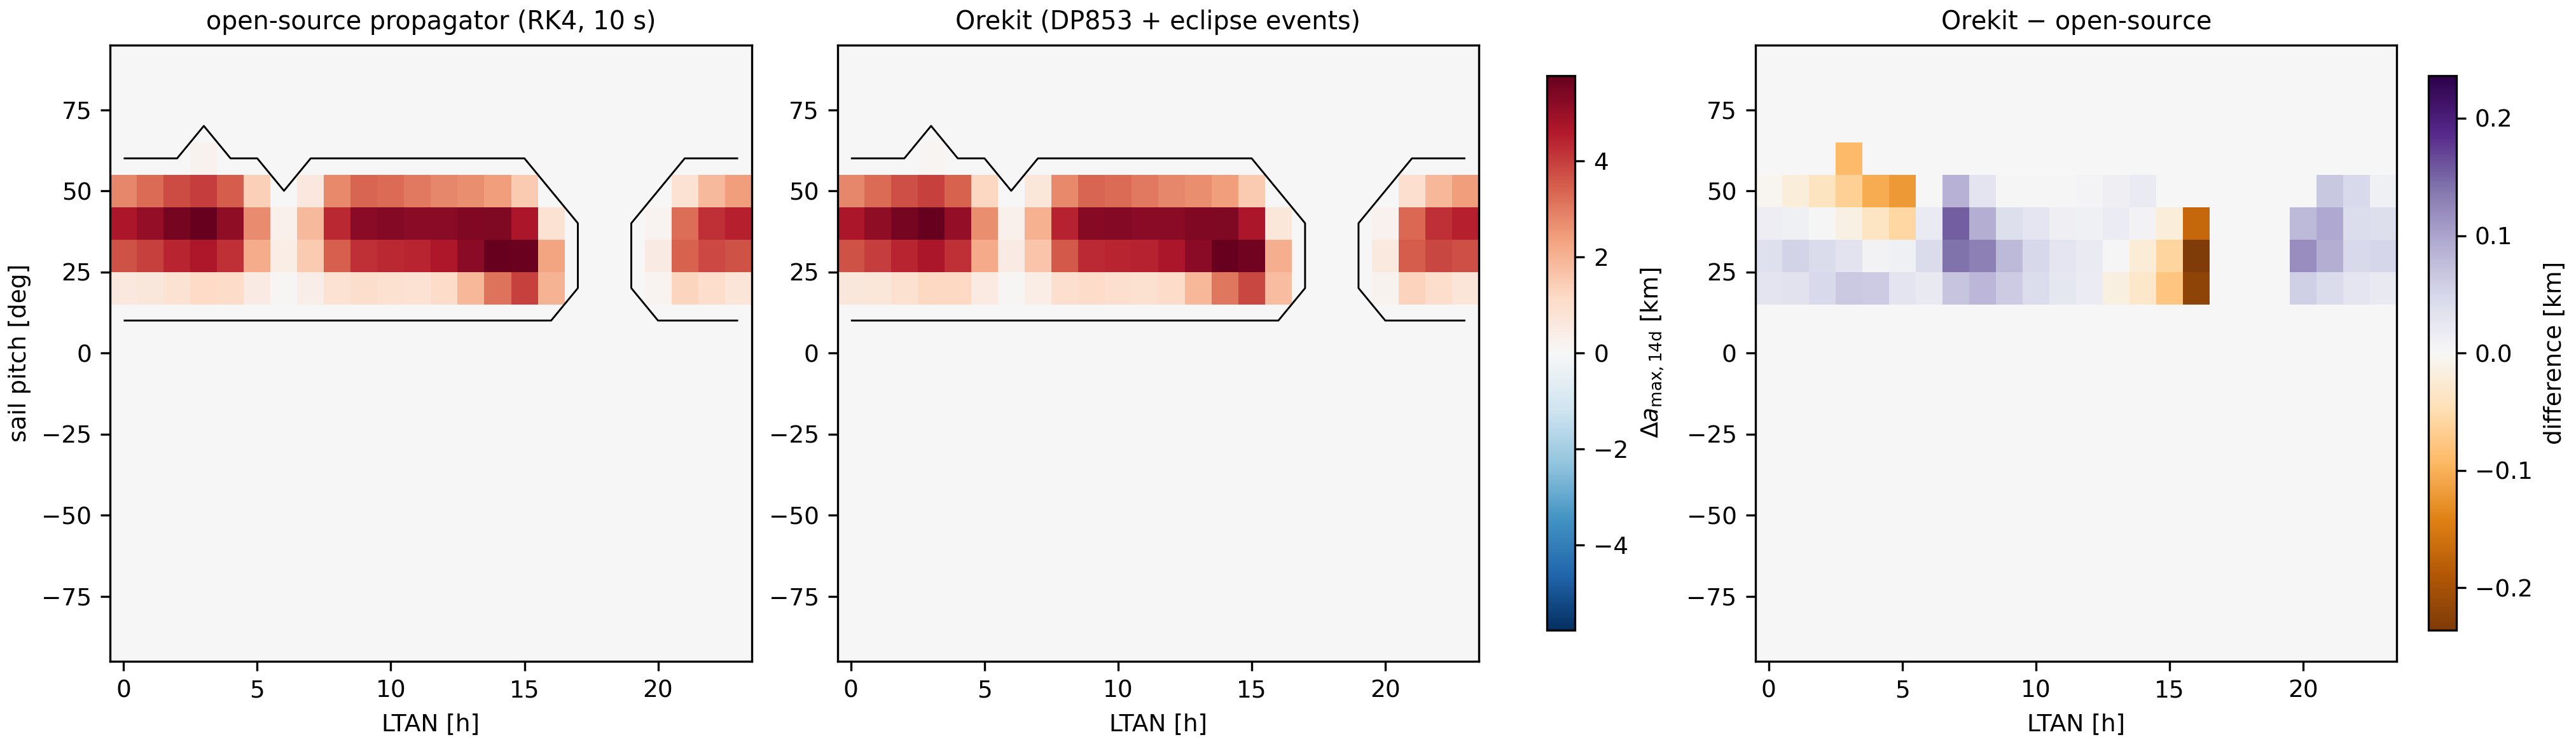
\includegraphics[width=1\linewidth]{Figures/r_map_orekit_compare.png}
    \setlength{\abovecaptionskip}{0pt}
    \caption{Independent reproduction of the \(800\,\mathrm{km}\) gain lobe. Left: \(\Delta a_{\max,14\mathrm{d}}\) from the open-source propagator on the \(24\times19\) cells common to the Orekit sweep (LTAN step \(1\,\mathrm{h}\), pitch step \(10^\circ\)). Centre: the same map from Orekit (DP853 with eclipse event detection). Right: the cell-by-cell difference (Orekit minus open-source). Both maps contain \(82\) positive cells, agree in sign everywhere and peak at LTAN \(14.0\,\mathrm{h}\), pitch \(+30^\circ\) (\(5.776\) and \(5.753\,\mathrm{km}\)); the RMS difference is \(0.029\,\mathrm{km}\) and the largest \(0.236\,\mathrm{km}\).}
    \label{fig:repro_lobe}
\end{figure*}

\begin{table*}[htbp]
\centering
\caption{Cross-validation against Orekit 13.1.7. Force gates are evaluated at \(198\) states along one orbit with a shared Sun position; propagated \(14\)-day values use RK4 at \(30\,\mathrm{s}\) in both tools and the node-sampled mean semi-major axis; the map, \(75\)-day and one-orbit rows use Orekit's DP853 integrator with eclipse event detection. Anchor LTAN \(14.0\,\mathrm{h}\), pitch \(+35^\circ\) unless stated.}
\label{tab:orekit}
\vspace{0.5em}
\footnotesize
\setlength{\tabcolsep}{3pt}
\begin{tabular}{>{\raggedright\arraybackslash}p{5.0cm} >{\raggedright\arraybackslash}p{2.4cm} >{\raggedright\arraybackslash}p{2.4cm} >{\raggedright\arraybackslash}p{2.8cm}}
\toprule
Quantity & Open-source & Orekit & Difference \\
\midrule
Gravity acceleration, relative & --- & --- & \(0\) \\
Drag acceleration, relative & --- & --- & \(7.4\times10^{-15}\) \\
SRP acceleration, relative & --- & --- & \(1.1\times10^{-15}\) \\
Eclipse flag & --- & --- & \(0\) mismatches \\
Sail normal from attitude & --- & --- & \(2.8\times10^{-17}\) \\
Plate force vs \(\cos^2\alpha\) law & --- & --- & \(1.5\times10^{-15}\) \\
\(J_2\) only, \(14\,\mathrm{d}\), \(700\,\mathrm{km}\) [km] & \(-0.01198\) & \(-0.01198\) & \(2.6\times10^{-10}\) \\
\(J_2\) only, \(14\,\mathrm{d}\), \(800\,\mathrm{km}\) [km] & \(-0.01128\) & \(-0.01128\) & \(2.7\times10^{-10}\) \\
\(J_2\) + spherical drag, \(14\,\mathrm{d}\), \(700\,\mathrm{km}\) [km] & \(-69.872\) & \(-69.872\) & \(4.0\times10^{-10}\) \\
\(J_2\) + spherical drag, \(14\,\mathrm{d}\), \(800\,\mathrm{km}\) [km] & \(-18.382\) & \(-18.382\) & \(2.8\times10^{-10}\) \\
Sun-facing area at pitch \(24.8^\circ\) [m\(^2\)] & \(90.78\) (analytic) & \(90.76\) & \(0.02\) \\
N-plate magnitude vs \(C_r\cos^2\alpha\), \(\alpha \le 45^\circ\) & --- & --- & \(\le 1.55\%\) \\
Full model, analytic Sun at \(1\,\mathrm{AU}\) [km] & \(+5.438\) & \(+5.605\) & \(0.181\) (max) \\
Full model, production Sun (\(1/d_{\odot}^2\) / DE-440) [km] & \(+5.933\) & \(+6.127\) & \(0.194\) (max) \\
Former \(700\,\mathrm{km}\) anchor, analytic Sun [km] & \(-21.478\) & \(-21.180\) & \(0.299\) (max) \\
Former \(700\,\mathrm{km}\) anchor, production Sun [km] & \(-21.158\) & \(-20.842\) & \(0.318\) (max) \\
\(800\,\mathrm{km}\) map, \(456\) common cells: positive cells & \(82\) & \(82\) & sign agreement \(100\%\) \\
\quad peak at (\(14.0\,\mathrm{h}\), \(+30^\circ\)) [km] & \(5.776\) & \(5.753\) & RMS \(0.029\), max \(0.236\) \\
\(75\,\mathrm{d}\): peak [km] (day) & \(+10.86\) (\(38.1\)) & \(+10.95\) (\(37.9\)) & \(0.09\) \\
\(75\,\mathrm{d}\): final [km] & \(-2.69\) & \(-2.37\) & \(0.32\) \\
One orbit: umbra fraction & \(32.1\%\) & \(32.0\%\) & \(0.1\%\) \\
One orbit: sign-selectivity & \(77.4\%\) & \(77.6\%\) & \(0.2\%\) \\
One orbit: SRP work, eclipse on [J\,kg\(^{-1}\)] & \(+310.3\) & \(+309.7\) & \(0.6\) \\
One orbit: SRP work, eclipse off [J\,kg\(^{-1}\)] & \(+1.4\) & \(+0.77\) & \(0.6\) \\
\bottomrule
\end{tabular}
\end{table*}

\subsection{Drag conventions and atmosphere models}
\label{sec:val_drag}
\noindent The STK comparison leaves drag as the one component whose propagated effect differs between tools, and Section~\ref{sec:sensitivity} shows that the regime boundary at \(800\,\mathrm{km}\) lies within a factor of two of the US-1976 density. Table~\ref{tab:drag_conventions} therefore separates the drag conventions from the atmosphere model with Orekit, propagating \(J_2\) plus spherical drag for \(14\) days (RK4 \(30\,\mathrm{s}\), node-sampled) and changing one element at a time. At \(700\,\mathrm{km}\) the baseline (US-1976, geocentric altitude, no co-rotation) gives \(-69.87\,\mathrm{km}\); a rigidly co-rotating atmosphere gives \(\times1.034\), the geodetic altitude \(\times0.816\), and the two together \(\times0.842\). At \(800\,\mathrm{km}\) the baseline is \(-18.38\,\mathrm{km}\) and the factors are \(\times1.024\), \(\times0.901\) and \(\times0.922\). The conventions are thus worth \(8\)--\(16\%\), and they account for the STK residual of Section~\ref{sec:val_stk} to within a few per cent. The atmosphere model is worth far more. Orekit's built-in Harris--Priester model multiplies the decay by \(7.08\) at \(700\,\mathrm{km}\), where the sail re-enters on day \(10.45\), and by \(3.15\) at \(800\,\mathrm{km}\); NRLMSISE-00 driven by the CSSI space-weather file for January 2026 multiplies it by \(2.57\) and \(1.59\). Because Orekit's built-in models are evaluated with their own conventions (geodetic altitude and co-rotation), these factors include the \(\times0.84\)--\(0.92\) convention effect, and the model effect proper is slightly larger.

\vspace{5pt}
\par\noindent A propagator-free check settles the question of scale raised by the reviewers. Integrating the secular rate \(\mathrm{d}a/\mathrm{d}t = -\rho\,C_D\,(A/m)\sqrt{\mu a}\) with the same density table along the decaying orbit gives \(-63.9\,\mathrm{km}\) at \(700\,\mathrm{km}\) and \(-17.6\,\mathrm{km}\) at \(800\,\mathrm{km}\), within \(8.5\%\) and \(4.2\%\) of the propagated \(-69.87\) and \(-18.38\,\mathrm{km}\); the remainder is the growth of eccentricity and the node-sampling convention. Holding the density at its \(700\,\mathrm{km}\) value instead gives about \(-43\,\mathrm{km}\), which is the reviewers' estimate: the difference is the density increase along the \(60\)--\(70\,\mathrm{km}\) of decay, not a defect of either tool. The three figures of the original submission are therefore reconciled as follows: \(-43\,\mathrm{km}\) is the constant-density estimate, \(-84\,\mathrm{km}\) was the value of the open-source propagator before the correction of the atmosphere table (Section~\ref{sec:model}), and \(-7\,\mathrm{km}\) was STK propagating a \(60\,\mathrm{kg}\) vehicle; the corrected values are \(-70\,\mathrm{km}\) (open-source, Orekit) and \(-60\,\mathrm{km}\) (STK, with its own conventions). At this altitude drag wins for every geometry (Figure~\ref{fig:heatmap_700km}) and the former anchor re-enters on day \(39.5\) (Table~\ref{tab:cases}).

\begin{table*}[htbp]
\centering
\caption{Drag conventions and atmosphere models in Orekit: \(14\)-day change of the node-sampled mean semi-major axis for \(J_2\) plus spherical drag (\(A/m = 10\,\mathrm{m^2\,kg^{-1}}\), \(C_D = 2.2\), RK4 at \(30\,\mathrm{s}\)), with the factor relative to the baseline of the paper (US-1976, geocentric altitude, no co-rotation). Orekit's built-in models use their own conventions (geodetic altitude, co-rotation); NRLMSISE-00 is driven by the CSSI space-weather file for January 2026. With Harris--Priester the \(700\,\mathrm{km}\) sail re-enters on day \(10.45\). The last row is the propagator-free secular integral with the same density table.}
\label{tab:drag_conventions}
\vspace{0.5em}
\footnotesize
\setlength{\tabcolsep}{4pt}
\begin{tabular}{l r r r r}
\toprule
& \multicolumn{2}{c}{\(700\,\mathrm{km}\)} & \multicolumn{2}{c}{\(800\,\mathrm{km}\)} \\
\cmidrule(lr){2-3} \cmidrule(lr){4-5}
Configuration & \(\Delta a(14\,\mathrm{d})\) [km] & factor & \(\Delta a(14\,\mathrm{d})\) [km] & factor \\
\midrule
Baseline (conventions of the paper) & \(-69.87\) & \(1.000\) & \(-18.38\) & \(1.000\) \\
Co-rotating atmosphere & \(-72.28\) & \(1.034\) & \(-18.82\) & \(1.024\) \\
Geodetic altitude & \(-57.04\) & \(0.816\) & \(-16.57\) & \(0.901\) \\
Co-rotating + geodetic & \(-58.82\) & \(0.842\) & \(-16.95\) & \(0.922\) \\
Harris--Priester (Orekit) & \(-494.7^{\dagger}\) & \(7.08\) & \(-57.84\) & \(3.15\) \\
NRLMSISE-00 (Orekit) & \(-179.9\) & \(2.57\) & \(-29.17\) & \(1.59\) \\
Analytic secular integral & \(-63.9\) & \(0.915\) & \(-17.6\) & \(0.958\) \\
\bottomrule
\end{tabular}
\par\vspace{2pt}
{\footnotesize \(^{\dagger}\)At re-entry, day \(10.45\).}
\end{table*}

\vspace{5pt}
\par\noindent The US-1976 profile is a static reference that carries no dependence on solar or geomagnetic activity (Section~\ref{sec:model}). To locate the regime boundary under a realistic thermosphere, the full model at the gain anchor was propagated for \(14\) days with the US-1976 baseline and with NRLMSISE-00 at constant low, moderate and high activity (\(F_{10.7} = 70\), \(140\) and \(200\); \(A_p = 4\), \(15\) and \(40\)) and with the CSSI space-weather file, at \(800\) and \(700\,\mathrm{km}\); Figure~\ref{fig:space_weather} and Table~\ref{tab:space_weather} report \(\Delta a_{\max,14\mathrm{d}}\) and \(\Delta a(14\,\mathrm{d})\).

\vspace{5pt}
\par\noindent At the \(800\,\mathrm{km}\) gain anchor the regime survives every atmosphere except the high-activity one. Under low activity (\(F_{10.7} = 70\), \(A_p = 4\)) the \(14\)-day gain rises to \(+13.18\,\mathrm{km}\), against \(+5.94\,\mathrm{km}\) with US-1976; under moderate activity (\(140\), \(15\)) it falls to \(+2.22\,\mathrm{km}\), with the CSSI space-weather file for January 2026 to \(+0.50\,\mathrm{km}\), and under high activity (\(200\), \(40\)) there is no gain at all (\(\Delta a_{\max,14\mathrm{d}} = 0\), \(\Delta a(14\,\mathrm{d}) = -45.5\,\mathrm{km}\)). The drag-only decays of the same runs, \(-2.33\), \(-9.90\), \(-12.72\), \(-14.43\) and \(-59.58\,\mathrm{km}\) respectively, show the cause: at this altitude and geometry the low-activity NRLMSISE-00 drag is about a quarter of the US-1976 value, the moderate level and the January 2026 file about \(1.3\) and \(1.5\) times it, and the high level about six times. At \(700\,\mathrm{km}\) the same geometry gains only under low activity (\(+10.69\,\mathrm{km}\); drag only \(-4.69\,\mathrm{km}\)); it decays with US-1976 (\(-13.77\,\mathrm{km}\); \(-31.15\,\mathrm{km}\) drag only), under moderate activity (\(-30.87\); \(-45.15\,\mathrm{km}\)) and with the CSSI file (\(-38.52\); \(-52.78\,\mathrm{km}\)), and under high activity it re-enters within the \(14\) days both with and without SRP.

\vspace{5pt}
\par\noindent The regime boundary therefore moves with the thermosphere. At \(800\,\mathrm{km}\) the gain survives under low and moderate activity, is marginal under the January 2026 conditions and closes under high activity; at \(700\,\mathrm{km}\) it exists only under low activity, where the quiet-Sun thermosphere is thinner than the static US-1976 profile. The US-1976 baseline of this paper thus lies between the low and moderate NRLMSISE-00 levels and slightly below the January 2026 conditions: it is neither the most favourable nor the least favourable case. The NRLMSISE-00 runs use Orekit's implementation with its own conventions (geodetic altitude, co-rotating atmosphere), and all runs use the DP853 integrator with eclipse event detection, so the US-1976 row of Table~\ref{tab:space_weather} is the DP853 reference of Section~\ref{sec:val_convergence} (\(+5.94\,\mathrm{km}\)) rather than the RK4 value of the maps.

\begin{table*}[htbp]
\centering
\caption{Space-weather dependence of the gain regime (Orekit, DP853 with eclipse event detection, \(14\) days, node-sampled mean semi-major axis): the full model and drag only at the gain-anchor geometry (LTAN \(14.0\,\mathrm{h}\), pitch \(+35^\circ\)) at \(800\) and \(700\,\mathrm{km}\) with the US-1976 baseline (conventions of the paper) and with Orekit's NRLMSISE-00 (geodetic altitude, co-rotation) at constant low, moderate and high activity (bracketed values are \(F_{10.7}\) and \(A_p\)) and with the CSSI space-weather file for January 2026. All values in km; for the full model \(\Delta a_{\max,14\mathrm{d}}\) / \(\Delta a(14\,\mathrm{d})\), for drag only \(\Delta a(14\,\mathrm{d})\). ``Re-entry'' marks runs whose perigee fell below \(120\,\mathrm{km}\) within the \(14\) days.}
\label{tab:space_weather}
\vspace{0.5em}
\footnotesize
\setlength{\tabcolsep}{3pt}
\begin{tabular}{>{\raggedright\arraybackslash}p{3.0cm} c r c r}
\toprule
& \multicolumn{2}{c}{\(800\,\mathrm{km}\)} & \multicolumn{2}{c}{\(700\,\mathrm{km}\)} \\
\cmidrule(lr){2-3} \cmidrule(lr){4-5}
Atmosphere model (activity) & full model & drag only & full model & drag only \\
& \(\Delta a_{\max,14\mathrm{d}}\) / \(\Delta a(14\,\mathrm{d})\) & \(\Delta a(14\,\mathrm{d})\) & \(\Delta a_{\max,14\mathrm{d}}\) / \(\Delta a(14\,\mathrm{d})\) & \(\Delta a(14\,\mathrm{d})\) \\
\midrule
US-1976 (baseline) & \(+5.940\) / \(+5.940\) & \(-9.899\) & \(0\) / \(-13.766\) & \(-31.152\) \\
NRLMSISE-00, low (70, 4) & \(+13.178\) / \(+13.178\) & \(-2.327\) & \(+10.685\) / \(+10.685\) & \(-4.685\) \\
NRLMSISE-00, moderate (\(140\), \(15\)) & \(+2.215\) / \(+2.213\) & \(-12.724\) & \(0\) / \(-30.872\) & \(-45.154\) \\
NRLMSISE-00, high (\(200\), \(40\)) & \(0\) / \(-45.455\) & \(-59.583\) & re-entry & re-entry \\
NRLMSISE-00, CSSI (Jan 2026) & \(+0.500\) / \(+0.499\) & \(-14.426\) & \(0\) / \(-38.517\) & \(-52.777\) \\
\bottomrule
\end{tabular}
\end{table*}

\begin{figure*}[htbp]
    \centering
    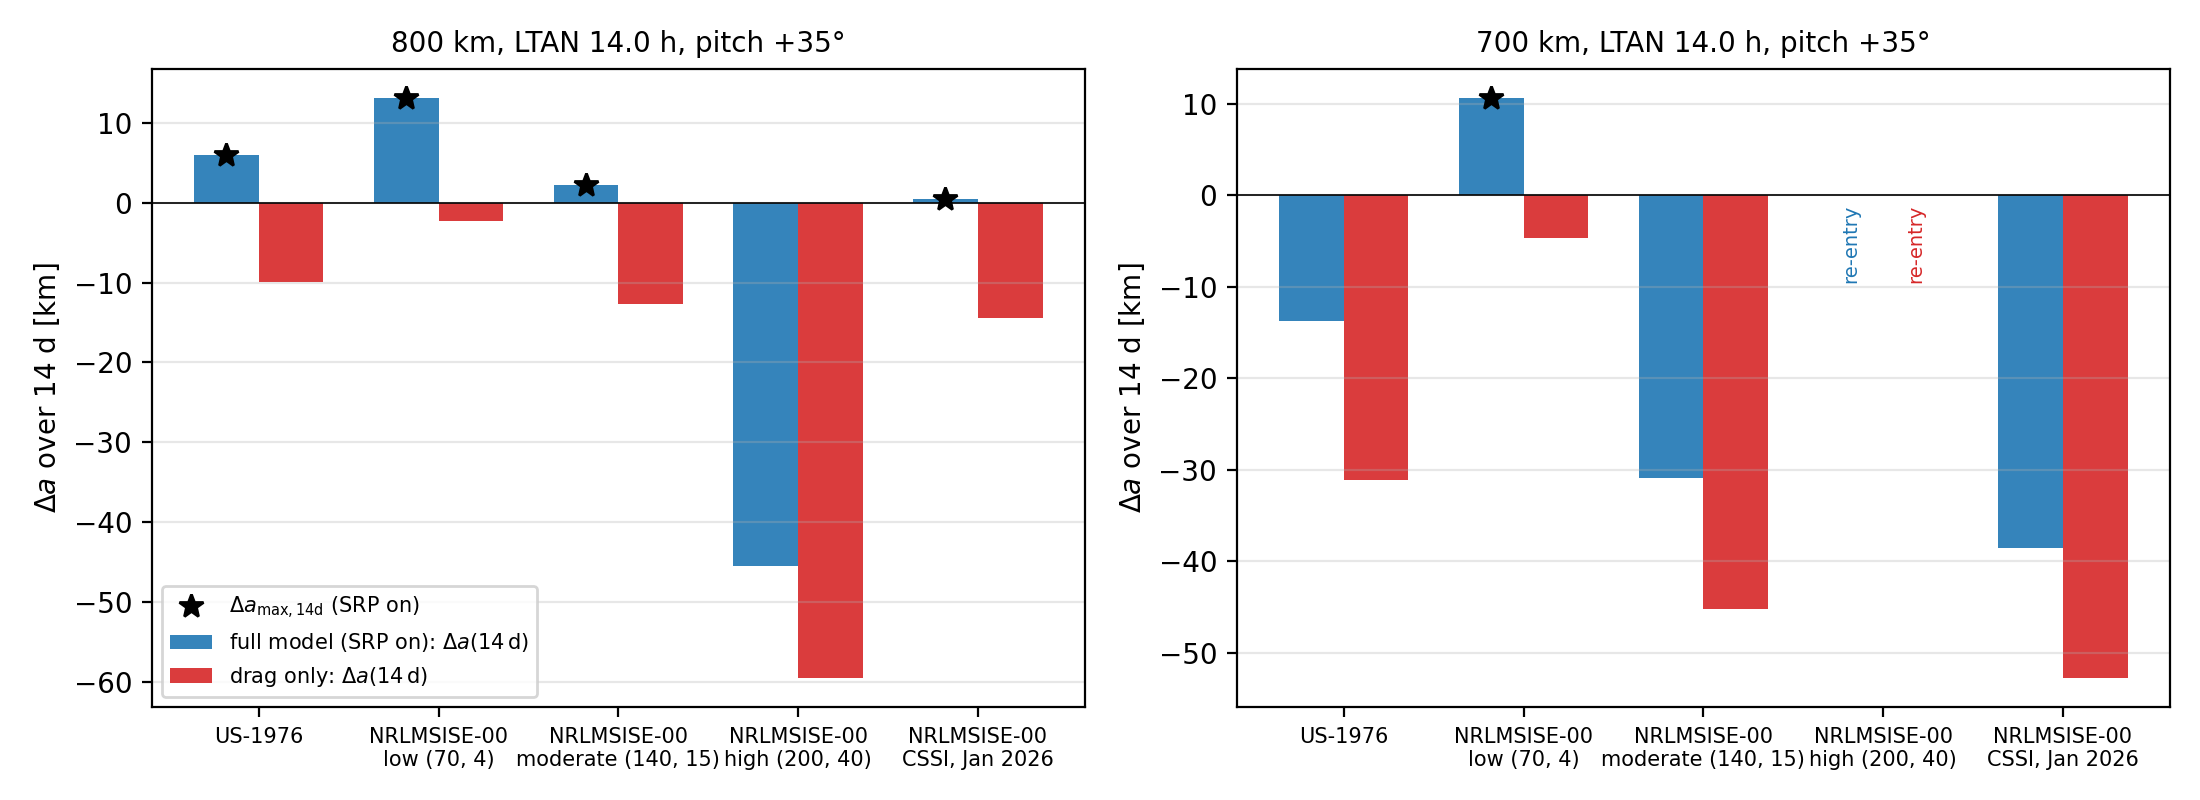
\includegraphics[width=1\linewidth]{Figures/r_space_weather.png}
    \setlength{\abovecaptionskip}{0pt}
    \caption{Space-weather dependence of the \(14\)-day response at the gain-anchor geometry (LTAN \(14.0\,\mathrm{h}\), pitch \(+35^\circ\)) at \(800\,\mathrm{km}\) (left) and \(700\,\mathrm{km}\) (right), from Orekit with DP853 and eclipse event detection. For each atmosphere model --- the US-1976 baseline and NRLMSISE-00 at constant low (\(F_{10.7} = 70\), \(A_p = 4\)), moderate (\(140\), \(15\)) and high (\(200\), \(40\)) activity and with the CSSI space-weather file for January 2026 --- the bars give \(\Delta a(14\,\mathrm{d})\) of the node-sampled mean semi-major axis for the full model (blue) and for drag only (red), and the stars mark \(\Delta a_{\max,14\mathrm{d}}\) of the full model where it is positive. The \(700\,\mathrm{km}\) runs under high activity re-enter within the \(14\) days and are marked ``re-entry''. The gain survives low and moderate activity at \(800\,\mathrm{km}\), is marginal under the January 2026 conditions and closes under high activity; at \(700\,\mathrm{km}\) it exists only under low activity.}
    \label{fig:space_weather}
\end{figure*}

\vspace{5pt}
\par\noindent These results are consistent with the density-multiplier sweep of Section~\ref{sec:sensitivity}, which places the drag-limited boundary at the gain anchor between \(1\times\) and \(2\times\) the US-1976 density at \(800\,\mathrm{km}\) and at or below \(0.5\times\) at \(700\,\mathrm{km}\). Judged by its drag-only decay, the low-activity atmosphere is equivalent to about a quarter of the US-1976 profile at \(800\,\mathrm{km}\) and gives \(+13.18\,\mathrm{km}\), close to the \(13.24\,\mathrm{km}\) of the \(0.25\times\) sweep point; the moderate level and the January 2026 file, at about \(1.3\times\) and \(1.5\times\), fall inside the band and still gain, by \(2.22\) and \(0.50\,\mathrm{km}\), so that the boundary at this geometry lies close to \(1.5\times\) the US-1976 density; high activity, at about \(6\times\), lies far beyond it, as does the Harris--Priester factor of \(3.15\) in Table~\ref{tab:drag_conventions}. At \(700\,\mathrm{km}\) the low-activity atmosphere is equivalent to about \(0.15\times\) the US-1976 profile, below the \(0.5\times\) threshold of the sweep, which is why a gain of \(+10.69\,\mathrm{km}\) appears there and nowhere else at that altitude. The mechanism of Sections~\ref{sec:physics} and \ref{sec:existence} is independent of the atmosphere model; the altitude and activity level at which it becomes net-positive are not, and the quantitative boundary must always be reported together with the atmosphere model and the activity level assumed.

\subsection{Note on the original submission}
\label{sec:val_note}
\noindent The quantitative results of Sections~\ref{sec:existence}--\ref{sec:sensitivity} in the originally submitted version of this paper were produced by a separate implementation of the same model, which was found during revision to contain errors in its aerodynamic incidence-angle convention, in its SRP coefficient and in its solar ephemeris. Those results have been withdrawn. Every result in the present version comes from the open-source propagator of Section~\ref{sec:val_propagator}, after the corrections described in this section, including the correction of the scale heights of the atmosphere table, which is now interpolated exponentially between the tabulated US-1976 values (Section~\ref{sec:model}). The two STK configuration errors of Section~\ref{sec:val_stkconfig} were found by the same read-back procedure, and the gain regime is now realised at \(800\,\mathrm{km}\) rather than at \(700\,\mathrm{km}\), where the corrected model is drag-dominated for every geometry.

\subsection{Data and software availability}
\label{sec:data}
\noindent The open-source propagator, the STK Astrogator build, probe and read-back scripts, the Orekit cross-validation study with its force gates and atmosphere experiments, the plate-definition files, the result files (JSON and NPZ) behind every number in this paper and the scripts that generate every figure and table are archived in the project repository \citep{svarogPropagatorCode2026}, so that the results of this section can be independently reproduced and extended.
\FloatBarrier



\section{Conclusions}
\label{sec:conclusion}
\FloatBarrier
\noindent This paper examined whether a passively oriented, spin-stabilised solar sail in near-polar low Earth orbit can exhibit a bounded interval of net orbital-energy gain under eclipse-modulated solar-radiation-pressure forcing. The results show that such a regime does exist, but only over a narrow and well-defined region of the sampled LTAN--pitch space. The gain response is therefore not a generic property of passive sailing in LEO, but a constrained transient effect that appears only under specific Sun-relative geometries.
\vspace{0.5em}
\par \noindent The results also show that eclipse is the causal enabler of this transient gain regime. In the representative gain case, the inclusion of eclipse produces positive short-horizon semi-major-axis growth, whereas removing eclipse from the same initial condition eliminates that behaviour and leads instead to clear decay. Orbit-resolved SRP work diagnostics show why: eclipse does not merely weaken SRP forcing, but selectively removes unfavourable portions of the SRP cycle. Under the gain geometry, this shifts the orbit-averaged SRP work balance positive; under neutral and decaying geometries, the same shadowing instead suppresses the positive recovery branch and leaves the net SRP contribution negative. The central physical result is therefore that eclipse timing can control the sign of the orbit-averaged SRP work input.
\vspace{0.5em}
\par \noindent At the same time, the longer-horizon behaviour shows unambiguously that this effect is transient and self-limiting rather than sustained. The representative gain trajectory initially exhibits semi-major-axis increase, but this does not correspond to uniform orbit raising. Instead, the orbit evolves through apogee growth, perigee erosion, and rising eccentricity, so that the early energy advantage progressively creates the conditions that undermine it. Drag becomes increasingly concentrated near perigee, while the favourable SRP projection weakens as the orbit distorts. As a result, the late-time orbit-averaged energy balance turns negative and the semi-major axis ultimately declines below its initial value. The transient gain regime identified here must therefore be understood as a front-loaded energy imbalance, not as evidence of persistent passive orbital uplift.

\noindent The sensitivity analysis supports the same interpretation. The gain-anchor case is not a numerically isolated point, but neither is it broadly robust. At lower altitude, the response is strongly limited by density and attitude offset; at higher altitude, the same geometry remains more tolerant over the sampled envelope, but still does not become a general passive orbit-raising solution. The mechanism is therefore physically real and interpretable, yet intrinsically bounded by geometry, atmospheric conditions, and the coupled eccentricity and drag penalties that emerge during the evolution.

\noindent Accordingly, the main contribution of this paper is not to propose sustained passive orbit raising in LEO, but to establish a narrower result: a constrained transient gain regime exists, eclipse timing is its causal enabler, and the same coupled dynamics that permit the early gain also drive its later breakdown. Future work should remain tightly focused on this mechanism, particularly on better analytical bounds for the gain window, broader mapping of the geometry dependence, and controlled studies of whether limited attitude variation --- informed by optimal steering approaches such as those described by \citet{dachwaldOptimalSolarSail2005} and \citet{mcinnes1999} --- can delay the eccentricity and drag-driven breakdown without changing the fundamentally transient character of the effect.
\FloatBarrier

\section*{Declaration of competing interest}
\par\noindent The authors declare that they have no known competing financial interests or personal relationships that could have appeared to influence the work reported in this paper.

\section*{Funding}
\par\noindent This work was supported by Imperial College London.

\section*{Data availability}
\par\noindent The open-source propagator, the STK Astrogator build and sweep scripts, the plate-definition files, the cross-validation utilities and all reproduced figures are openly available in the project repository \citep{svarogPropagatorCode2026}, as described in Section~\ref{sec:data}.

\section*{Acknowledgements}
\noindent The authors thank Dr.\ Aaron Knoll and Professor Matthew Santer for their guidance and support. We also gratefully acknowledge the REXUS/BEXUS programme and its partner organisations for supporting the wider Project Svarog team, including early prototyping activities that informed the broader development context of this work. The authors further thank Esmée Menting and Dr.\ Dorota Budzyn for their support of the project, and acknowledge the contributions of Gil Barbosa Ribeiro, Ivan Revenga Riesco, Golf Rojnuckarin, and Beatriz Soriano Tortosa to the team’s wider design effort. We also thank Imperial College London for providing funding and facilities that supported the project.

\vspace{5pt}
\par\noindent \textit{The REXUS/BEXUS programme is realised under a bilateral Agency Agreement between the German Aerospace Center (DLR) and the Swedish National Space Agency (SNSA). The Swedish share of the payload has been made available to students from other European countries through a collaboration with the European Space Agency (ESA). EuroLaunch, a cooperation between the Swedish Space Corporation (SSC) and the Mobile Rocket Base (MORABA) of DLR, is responsible for campaign management and launch operations. Experts from DLR, SSC, ZARM, and ESA provide technical support to the student teams throughout the project. REXUS and BEXUS are launched from SSC Esrange Space Center in northern Sweden.}

%% Loading bibliography style file
%% Acta Astronautica requires numbered references in square brackets,
%% numbered in order of first appearance in the text.
%% -num-names (not -num) so that \citet renders as "Author [10]" rather
%% than "(author?) [10]"; the reference list itself remains numbered.
\bibliographystyle{elsarticle-num-names}

% Loading bibliography database
\bibliography{cas-refs,D}

\end{document}

